\documentclass[justified]{tufte-handout}

\hypersetup{colorlinks}

\usepackage{aas_macros}
\usepackage{amsthm,amsmath,amssymb}
\usepackage{wasysym}
\usepackage{units}
\usepackage{setspace,graphicx,enumerate}
\usepackage{breqn,flexisym} % break equations over multiple lines
\usepackage{booktabs} % for nicely typeset tabular material
%\usepackage{fancyvrb,xspace}
%\fvset{fontsize=\normalsize}

\renewcommand{\b}{\boldsymbol}
\renewcommand{\v}{\vec}
\newcommand{\p}{\phantom}
\renewcommand{\d}{{\rm d}}

\title{Qual Review}
\author{Best Grad Students Ever}
\publisher{Department of Astronomy\\
           California Institute of Technology}

\begin{document}
\maketitle
\tableofcontents
\clearpage

\section{General Astronomy}
Some things we come across that aren't specific to any one class, but are 
good to have an idea of.

\begin{table}[H]
\centering
\begin{tabular}{c c}
\hline\hline
Band&$\lambda$\\
\hline
Radio&$>$100 cm\\
Microwave&10 mm-100 cm\\
IR&0.7 $\mu$m-10 mm\\
Optical&400-700 nm\\
UV&10-400 nm\\
Xray&10 pm-10 nm\\
$\gamma$ray&$<$10  pm\\
\hline\hline
\end{tabular}
\caption{Wavelengths of different parts of the Electromagnetic Spectrum}
\end{table}

\begin{table}[H]
\centering
\begin{tabular}{c c c}
\hline\hline
Band&$\lambda$ ($\mu$m)&$\frac{\Delta\lambda}{\lambda}$\\
\hline
U&0.36&0.15\\
B&0.44&0.22\\
V&0.55&0.16\\
R&0.64&0.23\\
I&0.79&0.19\\
J&1.26&0.16\\
H&1.60&0.23\\
K&2.22&0.23\\
\hline\hline
\end{tabular}
\caption{Wavelengths and widths of Johnson system photometric filters}
\end{table}

Good lines to know:
\begin{table}[H]
\centering
\begin{tabular}{c c c}
\hline\hline
Line&Transition&Wavelength (\AA)\\ \hline
Ly$\alpha$&$2\leftrightarrow 1$&1216\AA\\
Ly$\beta$&$3\leftrightarrow 1$&1025\AA\\
Ly$\gamma$&$4\leftrightarrow 1$&972\AA\\
Ly$_{con}$&$\infty\leftrightarrow 1$&911\AA\\
H$\alpha$&$3\leftrightarrow 2$&6563\AA\\
H$\beta$&$4\leftrightarrow 2$&4861\AA\\
H$\gamma$&$5\leftrightarrow 2$&4340\AA\\
H$_{con}$&$\infty\leftrightarrow 2$&3646\AA\\
\hline\hline
\end{tabular}
\caption{Common transitions of Hydrogen.}
\label{tab:spectral_lines}
\end{table}
I think we should know the exact wavelength for Ly$\alpha$,Ly$_{con}$,
H$\alpha$, and H$_{con}$.  Those are all important for other things (Lyman break galaxies, 
H ionization, Balmer jump...).  The other lines, maybe just have some idea of where they are.
Fun fact, the wavelength of Ly$\alpha$ is the address of Cahill!

\subsection{Magnitudes}
I can never remember the exact formulas for going between magnitudes and 
luminosities, so here they are:
\begin{equation}
m-M=5\log{\left(\frac{d}{10 pc}\right)}
\end{equation}
\begin{equation}
M=M_{\odot}-2.5\log{\left(\frac{L}{L_{\odot}}\right)}
\end{equation}
where $M_{\odot}=4.74$.  A difference of 5 magnitudes corresponds to a factor 
of 100 in luminosity.

\subsection{The Virial Theorem}
\newthought{The virial theorem} is a cute result of classical mechanics that can be generally
applied to many areas of astronomy.  Therefore we will treat it here without reference to
stars, galaxies, or the ISM.

Let's begin by thinking about a system of particles labeled with $i=1,\ldots,N$, and with
position and momentum denoted by $\b r_i$ and $\b p_i$ respectively.  By applying the non-relativistic
definition of momentum\sidenote{
    \begin{dmath*}
        \b p_i = m_i\dot{\b r_i}
    \end{dmath*},
    where $m_i$ is the mass of the $i$th particle.
}, we can show
\begin{dmath*}
    \frac{\d}{\d t}\sum_i \b p_i\cdot\b r_i
        = \frac{\d}{\d t}\sum_i m_i\dot{\b r_i}\cdot\b r_i
        = \frac{1}{2}\frac{\d^2}{\d t^2}\sum_i m_i r_i^2
\end{dmath*}.
The final sum is simply the total moment of inertia $I$ of the system\sidenote{
    \begin{dmath*}
        I \equiv \sum_i m_i r_i^2
    \end{dmath*}
}.

However, if we apply the product rule, we can also show
\begin{dmath*}
    \frac{\d}{\d t}\sum_i \b p_i\cdot\b r_i
        = \sum_i \frac{\d\b p_i}{\d t}\cdot\b r_i
            +\sum_i \b p_i\cdot\frac{\d\b r_i}{\d t}
        = \sum_i \b F_i\cdot\b r_i
            +\sum_i m_i{\dot r_i}^2
\end{dmath*}.
The final term we recognize as twice the kinetic energy of the system, $2K$.
Combining this with the previous result gives us the identity\sidenote{
    This is always true if classical mechanics holds!
}
\begin{dmath}
    \frac{1}{2}\frac{\d^2I}{\d t^2}
        = \sum_i \b F_i\cdot\b r_i+2K
\end{dmath}.

Now we specialize to the case of gravitational interactions\sidenote{
    That is, we require
    \begin{dmath*}
        \b F_i = -\sum_{j\neq i} \frac{Gm_im_j}{r_{ij}^3}(\b r_i-\b r_j)
    \end{dmath*}
}.  This implies
\begin{dmath*}
    \sum_i \b F_i\cdot\b r_i
        = -\sum_i\sum_{j\neq i} \frac{Gm_im_j}{r_{ij}^3}(\b r_i-\b r_j)\cdot \b r_i
        = -\sum_i\sum_{j > i} \frac{Gm_im_j}{r_{ij}}
\end{dmath*}.
The final expression is that of the total gravitational potential energy $\Omega$
of the system\sidenote{
    The limit on the second sum is necessary to prevent double-counting.
}.  This gives us the virial theorem
\begin{dmath}\boxed{
    \frac{1}{2}\frac{\d^2I}{\d t^2}
        = \Omega+2K
}\end{dmath}.
A system is said to be virialized if $\d^2I/\d t^2=0$, in which case
\begin{dmath}\boxed{
    \Omega+2K = 0
}\end{dmath}.

Although, we assumed purely gravitational interactions, random thermal collisions
do not contribute to $\sum_i\b F_i\cdot\b r_i$ because the direction of the force is
randomized.  This means we have a very general relation that relates the gravitational potential
energy to the kinetic energy of virialized systems.  Note that virialized systems are
bound because $\Omega+K < 0$.

Here's a description from Astrophysics in a nutshell.  
Start with the hydrostatic equilibrium equation, multiply both sides by $4\pi r^3dr$, and integrate:
\begin{equation}
\int_0^R4\pi r^3\frac{dP}{dr}\,dr = -\int_0^R\frac{GM(r)\rho (r)4\pi r^2}{r}\,dr
\end{equation}
The right hand side is just the total gravitational energy in the star.  The left hand side 
can be integrated by parts to give
\begin{equation}
[P(r)4\pi r^3]_0^R-3\int_0^RP(r)4\pi r^2\,dr
\end{equation}
The first term is 0 because pressure goes to 0 at the surface.  The second term is average 
pressure times volume, so 
\begin{equation}
\bar{P}=-\frac{1}{3}\frac{E_{gr}}{V}
\end{equation}
Using the ideal gas law and the thermal energy of a gas ($\frac{3}{2}NkT$), can show
\begin{equation}
P=\frac{2}{3}\frac{E_{th}}{V}
\end{equation}
So, 
\begin{equation}
\boxed{E_{th}=-\frac{E_{gr}}{2}}
\end{equation}
which is the Virial theorem.  This is why stars have a negative heat capacity and evolve the way 
they do.  If they contract (making $E_{gr}$ more negative), the thermal energy (temperature) 
increases.


\subsection{Timescales}
\newthought{The free-fall timescale} describes the length of time an object takes to collapse
under the influence of gravity if its pressure support is removed.  The collapse of a star
during a supernova occurs on the free-fall timescale.
If the Sun had no pressure support and just collapsed under gravity, it's velocity would be 
determined by energy conservation:
\begin{equation}
\frac{1}{2}\left(\frac{dr}{dt}\right)^2 = \frac{GM}{r}-\frac{GM}{r_0}
\end{equation}
assuming the mass interior to any element is constant (the entire cloud collapse all at once).
This equation can be integrated to give
\begin{equation}
\tau_{ff}=\left(\frac{r_0^3}{2GM}\right)^{1/2}\int_0^1\left(\frac{x}{1-x}\right)^{1/2}\,dx
\end{equation}
The definite integral is equal to $\pi/2$, so
\begin{equation}\boxed{
\tau_{ff}=\left(\frac{3\pi}{32G\rho}\right)^{1/2}
}\end{equation}
Free fall time for the Sun is 1800 seconds.

\newthought{The Kelvin-Helmholtz timescale} is the relevant timescale for an object to
radiate away its energy.  Gas clouds collapse into protostars on the Kelvin-Helmholtz timescale,
and stellar cores contract on the Kelvin-Helmholtz timescale when they run out of nuclear fuel.

Michael will fill this out eventually...

\newthought{The two-body relaxation timescale} describes how long it takes
a body (in a gravitationally interacting system) to have its velocity perturbed by other bodies
in the system.  A short relaxation time implies that close encounters between stars are more
likely.  A ``relaxed system'' that is several relaxation timescales old has a centrally
condensed core with a diffuse halo.

To derive the relaxation timescale, imagine a star passing by another star with mass $m$ and
impact parameter $b$.  We assume that the gravitational interaction is small so that
to zeroth order the path of the first star is linear, unperturbed by the gravity of $m$.
Due to symmetry considerations, the acceleration due to gravity parallel to the path
averages to zero over the duration of the interaction.  So we only need to consider the
perpendicular acceleration:
\begin{dmath}
    a_\perp = \frac{Gm}{x^2+b^2}\frac{b}{\sqrt{x^2+b^2}}
\end{dmath},
where $x$ is the position of the first star along its path\sidenote{
    If you need help imagining the geometry here, ask Michael, he's a little too lazy to try
    and draw a diagram right now.
}, running from $-\infty$ to $+\infty$.  The total perturbation to the perpendicular velocity
is therefore given by
\begin{dgroup*}
\begin{dmath*}
    \delta v_\perp = \int_{-\infty}^{+\infty} a_\perp \frac{\d x}{v}
                   = \frac{Gmb}{v}\int_{-\infty}^{+\infty} \frac{\d x}{(x^2+b^2)^{3/2}}
\end{dmath*}
\begin{dmath}
    \p{\delta v_\perp}
                   = \frac{2Gm}{bv}
\end{dmath}.
\end{dgroup*}
These interactions occur in a random direction so that $\langle\delta v_\perp\rangle=0$.
However $\langle\delta v_\perp^2\rangle > 0$, so we will be interested in how these
interactions affect the square of the velocity (the kinetic energy).
The rate of these interactions at a given $b$ is $nv\cdot2\pi b\d b$ where $n$ is the number
density of these stars.  Therefore
\begin{dmath*}
    \frac{\d}{\d t} \langle\delta v_\perp^2\rangle
        = \int_{b_{\rm min}}^{b_{\rm max}} \delta v_\perp^2 \cdot nv \cdot 2\pi b\d b
        = \frac{8\pi G^2m^2n}{v}\int_{b_{\rm min}}^{b_{\rm max}} \frac{\d b}{b}
        = \frac{8\pi G^2m^2n}{v} \ln\left(\frac{b_{\rm max}}{b_{\rm min}}\right)
\end{dmath*}.
The maximum impact parameter is the radius of the system $R\sim(N/n)^{1/3}$ where
$N$ is the total number of stars.  The minimum impact parameter is roughly the
inter-star spacing or $n^{-1/3}$ so that $\ln(b_{\rm max}/b_{\rm min}) \sim (\ln N)/3$.
Finally we have the relaxation timescale
\begin{dmath}\boxed{
    \tau_{\rm relax} = \frac{v^2}{\frac{\d}{\d t}\langle\delta v_\perp^2\rangle} \nolinebreak
                     = \frac{3v^3}{8\pi G^2m^2n\ln N}
}\end{dmath}.





\section{Radiative Processes}

Remember guys, there's nothing funny about neutrinos.

\subsection{Questions}\label{sec:rad_will_ask}

\begin{enumerate}

\item \textbf{Derive the total power and characteristic frequency of synchrotron radiation from
      a relativistic particle of mass m, charge e, and energy E moving in a magnetic field B.
      Use this to explain why synchrotron radiation is generally negligible for protons.}
      
      \newthought{Synchrotron radiation is}
      caused by relativistic charged particles moving in an external
      magnetic field. Therefore, the Lorentz force equations of motion and the Larmor formula
      for the power radiated by an accelerating charged particle will be relevant. 
      \begin{dgroup}
      \begin{dmath}
        \text{Lorentz Force:}\quad F_{B} = \frac{q}{c} \v{v} \times \v{B}
      \end{dmath}
      \begin{dmath}
        \text{Larmor Formula:}\quad P = \frac{2}{3} \frac{q^{2}}{c^{3}} \gamma^{4} a^{2}
      \end{dmath}
      \end{dgroup}
      Use the equations of motion to solve for the acceleration, $a$, of the particle and plug
      into the Larmor formula to get the total power radiated from a single particle.
      \begin{dgroup*}
      \begin{dmath*}
            F_{B} = \frac{\d}{\d t} (\gamma m \v{v})
      \end{dmath*}
      \begin{dmath*}
            \frac{q}{c} \v{v} \times \v{B} = \gamma m \frac{\d\v v}{\d t},
      \end{dmath*}
      \end{dgroup*}
      where we have used the fact that $\gamma$ is constant\sidenote{
        From the definition of work:
        \begin{dgroup*}
        \begin{dmath*}
        \d W = \v F\cdot \v{\d s}
        \end{dmath*}
        \end{dgroup*}
        However, the Lorentz force $F_B$ is always perpendiculr to $\v{\d s}$ so that
        no work is done on the particle.  Therefore the speed (and hence $\gamma$) is constant.
      }.
      
      Now the acceleration can be solved for directly. In the direction of $\v B$,
      there is no acceleration (remember the cross product). Perpendicular to $\v B$:
      \begin{equation}
        \left(\frac{\d v}{\d t}\right)_{\perp} = \frac{q}{\gamma mc} vB \sin{\alpha},
      \end{equation}
      where $\alpha$ is the angle between the velocity and the magnetic field.
      Plug into the Larmor Formula to get the total power radiated by a single electron:
      \begin{dmath}
        P = \frac{2}{3} \frac{q^{4}B^{2}}{c^{5}m^{2}} \gamma^{2} v^{2} \sin^2{\alpha}
      \end{dmath}
      Averaging over the pitch angle $\alpha$ and using the definition of the Thomson
      cross-section, we find
      \begin{dmath}\boxed{
        P = \frac{4}{3} \sigma_T c\beta^2\gamma^2\frac{B^2}{8\pi}
      }\end{dmath}
      
      \newthought{The characteristic frequency} of synchrotron emission is influenced
      by two effects: the gyro-frequency\sidenote{
        The frequency at which a relativistic electron gyrates in a constant magnetic field.
      }, and relativistic beaming.

      The opening angle of the cone of emission (due to the beaming) is $\sim2/\gamma$.
      Therefore an observer can only see the emission during the time it takes the electron
      to travel $2/\gamma$ radians along its circular orbit.  This corresponds to an arclength
      of $2r/\gamma$ where $r$ is the Larmor radius\sidenote{
        The radius of an electron's orbit in a uniform magnetic field.  Begin by equating
        the Lorentz force with the centripetal force:
        \begin{dgroup*}
        \begin{dmath*}
            \frac{qvB}{c}\sin\alpha = \frac{\gamma mv^2}{r}
        \end{dmath*}
        \begin{dmath*}
            r = \frac{\gamma mvc}{qB\sin\alpha}
        \end{dmath*}
        \end{dgroup*}
      }.
      Therefore, if the electron is moving with a speed $v$, it is only visible for a time
      \begin{dmath}
        \Delta t = \frac{2r}{\gamma v}\nolinebreak=\nolinebreak \frac{2mc}{qB\sin\alpha}
      \end{dmath}.
      However, the light emitted at the beginning of the pulse has to travel an extra
      distance $2r/\gamma$ (assuming $\gamma \gg 1$ we can treat the arc as a straight line).
      The distance in arrival time between the beginning and the end of the pulse is then
      \begin{dmath}
        \Delta t^\star = \Delta t - \frac{2r}{\gamma c}
            \nolinebreak=\nolinebreak \Delta t\left(1-\frac{v}{c}\right)
            \nolinebreak\approx\nolinebreak \frac{\Delta t}{2\gamma^2}
      \end{dmath},
      where the approximation\sidenote{
        \begin{dmath*}
            \frac{1}{\gamma^2} = 1-\frac{v^2}{c^2} = \left(1-\frac{v}{c}\right)\left(1+\frac{v}{c}\right)
                \approx 2\left(1-\frac{v}{c}\right)
        \end{dmath*}
      } requires $\gamma \gg 1$.

      The Fourier transform of the pulse shape gives the frequency structure of the synchrotron
      emission, however, because the pulse width is $\approx\Delta t^\star$, we the largest
      contribution to the Fourier integral will be modes with $\nu\sim1/\Delta t^\star$.
      Therefore we define the critical frequency to be
      \begin{dmath}\boxed{
        \nu_c \sim \frac{1}{\Delta t^\star} \nolinebreak=\nolinebreak \frac{\gamma^2 qB\sin\alpha}{mc}
      }\end{dmath}.

      The question asks for the synchrotron spectrum as a function of energy (not $\gamma$).
      Simply set $\gamma = E/mc^2$ in the above equations to eliminate $\gamma$.  Finally note
      that protons are $\sim 1800$ times more massive than electrons.

\item \textbf{Explain the connection between detailed balance, the Einstein A and B relations,
      Kirchoff's law and the Milne relations, and give an example of their use to connect the
      bremsstrahlung emission spectrum and the free-free absorption coefficient.}
      
      \newthought{Let's begin with} detailed balance\sidenote{
        Any ideas on what distinguishes detailed balance from un-detailed balance?
      }.  Detailed balance is simply a statement that there are an equal number of transitions
      into and out of a given state.
      \begin{dmath}
        \text{rate of transitions into state A} = \text{rate of transitions out of state A}
      \end{dmath}
      Einstein's coefficients tell us how to express this idea mathematically
      for radiative transitions\sidenote{
        Transitions that involve the emission or absorption of a photon.
      }.
      Consider a two state system where state (1) has a lower energy than state (2).
      Given an incident mean intensity (averaged over the line profile\sidenote{
        The mean intensity is
        \begin{dmath*}
            J_\nu\equiv\frac{1}{4\pi}\int I_\nu\d\Omega
        \end{dmath*},
        and averaging over the line profile gives us
        \begin{dmath*}
            \bar J = \int J_\nu\phi(\nu)\d\nu
        \end{dmath*}.
      }),
      $A_{21}$ is the probability of spontaneous emission per unit time,
      $B_{12}\bar J$ is the probability of absorption per unit time, and
      $B_{21}\bar J$ is the probability of stimulated emission per unit time.
      Detailed balance therefore tells us (for this two-state system) that
      \begin{dmath}\label{eq:detailed_balance}
        n_2A_{21} = (n_1B_{12}-n_2B_{21})\bar J
      \end{dmath}.
      In thermodynamic equilibrium (and with Maxwell-Boltzmann statistics\sidenote{
        This means spin-statistics aren't important.  We aren't dealing with bosons
        or fermions here.
      }), we have
       \begin{dmath}
        \frac{n_2}{n_1} = \frac{g_2}{g_1} e^{-h\nu_0 / k_B T}
       \end{dmath},
       where $h\nu_0 = E_2-E_1$ is the energy difference between the two levels,
       $E_2 - E_1$, such that taken together with detailed balance
       \begin{dmath}
        \bar J = \frac{A_{21}/B_{21}}{\frac{g_1B_{12}}{g_2B_{21}}e^{h\nu_0/kT}-1}
       \end{dmath}
       In thermodynamic equilibrium (with a narrow line profile), the
       line-averaged mean intensity is given by the Planck function\sidenote{
        \begin{dmath*}
            \bar J = B_\nu\nolinebreak= \frac{2h\nu^3}{c^2}\frac{1}{e^{h\nu/kT}-1}
        \end{dmath*}
       }.  Therefore we must have
       \begin{dgroup}
       \begin{dmath}\boxed{
        g_1B_{12} = g_2B_{21}
       }\end{dmath},
       \begin{dmath}\boxed{
        A_{21} = \frac{2 h \nu^3}{c^2}B_{21}
       }\end{dmath}.
       \end{dgroup}
       These are called the Einstein relations.
      Even though we assumed thermodynamic equilibrium, these relations do not depend on
      temperature and just describe properties of the atoms. Therefore, we can say they are more
      general and hold for cases that are not in thermodynamic equilibrium.
      Also, the A and B coefficients are intrinsic properties of individual 
      atoms, so they should have nothing to do with the overall state of the 
      gas and whether or not it's in thermodynamic equilibrium.

      \newthought{Now let's discuss} Kirchoff's law.
      Take a thermally emitting (not necessarily blackbody) material at temperature $T$ and place it 
      in a blackbody cavity also at temperature $T$.  With just the cavity, $I_{\nu}=B_{\nu}$
      (by definition of the Planck function $B(\nu)$).  
      With the material added, we still have a cavity of temperature $T$, so the total intensity must 
      still be a blackbody, since by definition this intensity does not depend on the internal 
      structure.  The added material has some source function $S_{\nu}$ that affects the total 
      intensity of the cavity.  Think of the new material as a new piece of the cavity, with radiation 
      contributed by its source function.  If the source function is greater than the blackbody function 
      of the cavity, too much radiation will be contributed and the resulting intensity will also be 
      greater than the blackbody of the cavity on its own.  If the source function is less than the 
      blackbody function, too little radiation will be contributed, decreasing the total intensity to 
      below the blackbody function.  But we know the total intensity must still be a blackbody function 
      of temperature $T$.
      So, we must have 
      \begin{dmath}\boxed{
        S_\nu = B_\nu
      }\end{dmath},
      and, by definition of $S_{\nu}$,
      \begin{dmath}\boxed{
        j_\nu = \alpha_\nu B_\nu
      }\end{dmath}.
      To clarify, the source function of a material in thermodynamic equilibrium is the
      Planck function\sidenote{
        This introduces an important distinction: \emph{thermal radiation} implies $S_\nu=B_\nu$,
        while \emph{blackbody radiation} implies $I_\nu=B_\nu$.
      }.
      
      We can relate the Einstein coefficients to the emission and absorption coefficients
      by noting that each transition adds or removes $h\nu$ in energy, spread over a solid
      angle of $4\pi$.  Therefore
      \begin{dgroup}
      \begin{dmath}\boxed{
        j_\nu = \frac{h \nu}{4 \pi} n_2 A_{21} \phi(\nu)
      }\end{dmath},
      \begin{dmath}\boxed{
        \alpha_\nu = \frac{h \nu}{4 \pi} (n_1 B_{12} - n_2 B_{21} ) \phi(\nu)
      }\end{dmath}.
      \end{dgroup}

      \newthought{Now the Milne relations} are the equivalent to the Einstein relations for
      photoionization / recombination (rather than transitions between energy levels in an atom).
      Following Rybicky \& Lightman (see p.\,284 for more discussion), assume we have a thermal
      velocity distribution of electrons\sidenote{
        The Maxwell-Boltzmann velocity distribution is
        \begin{dmath*}
        f(v)\,\d v = 4\pi\left(\frac{m}{2\pi kT}\right)^{3/2}v^2e^{-mv^2/2kT}\,\d v
        \end{dmath*}.
      } and that the radiation field is described by the Planck
      function $B_\nu$.
      Let $\sigma_{\rm fb}(v)$ be the cross section for an electron with speed $v$ to recombine
      with an ion, and let $\sigma_{\rm bf}(\nu)$ be the cross section for an ion to to be
      photoionized by a photon with frequency $\nu$. We can write the rate of recombinations
      and ionizations
      per volume (s$^{-1}$ cm$^{-3}$) in terms of the number densities of ions and electrons,
      the cross section, and the electron velocity distribution for a velocity range $dv$:
      \begin{dgroup}
      \begin{dmath}
      R_{\rm recomb} = N_+N_e \sigma_{\rm fb} f(v)v\,\d v
      \end{dmath}
      \begin{dmath}
      R_{\rm ioniz} = \frac{4\pi}{h\nu} N_n \sigma_{\rm bf} (1 - e^{-h\nu/k_{\rm B}T}) I_\nu\,\d\nu
      \end{dmath}
      \end{dgroup}
      The factor of $(1-e^{-h\nu/kT})$ apparently accounts for stimulated recombinations.
      Setting these two expressions equal (ie. assume detailed balance), and using the Planck
      function, the Maxwellian velocity distribution, and the Saha equation\sidenote{
        The Saha equation is
        \begin{dmath}
        \frac{N_+N_e}{N_n} = \left(\frac{2\pi mkT}{h^2}\right)^{3/2}\frac{g_eg_+}{g_n}e^{-\chi/kT}
        \end{dmath},
        where $\chi$ is the ionization potential.
      } it can be shown\sidenote{
        Note that $h\nu=mv^2/2+\chi$ and therefore $mv\,\d v=h\,d\nu$.
      } that
      \begin{dmath}\boxed{
      \frac{\sigma_{\rm bf}}{\sigma_{\rm fb}} = \frac{m^2 v^2 c^2}{h^2\nu^2}\frac{g_e g_+}{2g_n}
      }\end{dmath}.
      
      The Einstein relations, Milne relations, and Kirchoff's law all describe relationships
      between the absorption and emission of photons. Einstein deals with transitions between
      two energy levels on an atomic level using the properties and thermal distributions of
      atoms. Milne is the analogous relationship for ionization and radiative recombination.
      Kirchoff's law relates the absorption and emission coefficients in thermodynamic
      equilibrium.
      Kirchoff's law and the Einstein relations both relate emission and 
      absorption of photons, but Kirchoff's law only holds for thermal 
      radiation.  The Einstein relations are more general and extend Kirchoff's 
      law to non-thermal radiation processes.
      
      \newthought{In the case of bremsstrahlung}, the emission process is much easier to think
      about the reverse absorption process.  However, given Kirchoff's law and an expression
      for $j_\nu$ (see Section~\ref{sec:bremsstrahlung} for a derivation), the absorption
      coefficient is simply
      $\alpha_\nu = j_\nu / B_\nu$.  Recalling that $j_\nu = \epsilon_\nu/4\pi$, we have
      \begin{dgroup}
      \begin{dmath}
      \epsilon_{\nu}^{ff}=6.8\times10^{-38}T^{-1/2}Z^2n_en_ie^{-h\nu/kT}\overline{g_{ff}}ergs/s/cm^3/Hz
      \end{dmath}
      \begin{dmath}
      \alpha_{\nu}^{ff}=3.7\times10^8T^{-1/2}Z^2n_en_i\nu^{-3}(1-e^{-h\nu/kT})\overline{g_{ff}}cm^{-1}
      \end{dmath}.
      \end{dgroup}
      
\item \textbf{Draw the energy levels of the hydrogen atom and identify which transitions are
      allowed. Which ones are in the visible part of the spectrum? Which level has no
      allowed decays, and what is its main decay mode?}

      \marginnote{
      \begin{center}\begin{tabular}{cccc}
      $\vdots$ & $\vdots$ & $\vdots$ & $\vdots$ \\
      4s & 4p & 4d & 4f \\
      3s & 3p & 3d &\\
      2s & 2p &&\\
      1s &&&\\
      \end{tabular}\end{center}
        The above sketch shows the energy levels of the hydrogen atom (ignoring fine structure).
        The first number is the principal quantum number, usually denoted by $n$.
        The second letter denotes the orbital angular momentum $l$, where s, p, d, and f denote
        $l=1,\,2,\,3,\,4$ respectively.  The energy of a state is given by
        $E_n = -13.6\,{\rm eV}/n^2$.
      }

      \newthought{The allowed transitions}
      between states are governed by so-called ``selection rules.''
      This, however, is a misnomer because every transition is allowed, some are just strongly
      disfavored over others.  The most likely transitions (the ``allowed transitions'') are
      the electric dipole transitions which follow the following rules (in a one electron atom):
      \begin{dgroup}
      \begin{dmath}
        \Delta l = \pm 1
      \end{dmath}
      \begin{dmath}
        \Delta m = 0,\,\pm1
      \end{dmath}
      \end{dgroup}
      Keeping these selection rules in mind, and looking at sketch in the margins,
      the only state that has no allowed decays is the 2s state.  Its main decay mode is through
      the spontaneous emission of two photons.
      
      As far as optical transitions go, the 4 lowest energy Balmer transitions (transitions
      to $n=2$) are visible.  Table~\ref{tab:spectral_lines} gives a little more detail.

\end{enumerate}

\subsection{Specific intensity}
\newthought{The specific intensity} $I_{\nu}$ = energy per time per area per frequency per
steradian (erg/s/Hz/ster/cm$^2$).

\begin{table}[ht]
\centering
\begin{tabular}{ccc}
\toprule
Name & Units & Expression \\
\midrule
Specific mean intensity & erg/s/cm$^2$/Hz &
    $J_{\nu}=\frac{1}{4\pi}\int I_{\nu}\,d\Omega$ \\
Specific energy density & erg/cm$^3$/Hz &
    $u_{\nu}=\frac{4\pi}{c}J_{\nu}$ \\
Energy Flux & erg/s/cm$^2$/Hz &
    $F_{\nu}=\int I_{\nu}\cos \theta\,d\Omega$ \\
Momentum Flux &&
    $p_{\nu}=\frac{1}{c}\int I_{\nu}\cos^2 \theta\,d\Omega$ \\
\bottomrule
\end{tabular}
\caption{Moments of the specific intensity}
\label{tab:moments}
\end{table}

\subsection{Radiative Transfer}
\newthought{In steady state},
with no scattering, along a path $s$, change in intensity is emission - absorption.
\begin{dmath}\frac{dI_{\nu}}{ds}=j_{\nu}-\kappa_{\nu}I_{\nu}\end{dmath}
where $\kappa_{\nu}=\text{absorption opacity}=n\sigma=1/\lambda_{\nu}$ and $j_{\nu}$ is 
defined as the energy emitted per unit volume per steradian per second per Hz.  This is similar 
to emissivity, except emissivity ($\epsilon_{\nu}$) is per unit mass, not per unit volume.
An alternate for of the radiative transfer equation is 
\begin{dmath}\boxed{\frac{dI_{\nu}}{d\tau_{\nu}}=-I_{\nu}+S_{\nu}}\end{dmath}
$S_{\nu}=\frac{j_{\nu}}{\kappa_{\nu}}$ is the source function and $d\tau_{\nu}=\kappa_{\nu}ds$ 
is measured along the path of the light ray (from the source to the observer).  If optical depth 
is measured from the observer to the source, $d\tau_{\nu}$ picks up a negative sign, and the 
equation becomes
\begin{dmath}\frac{dI_{\nu}}{d\tau_{\nu}}=I_{\nu}-S_{\nu}\end{dmath}
A few solutions to the radiative transfer equation are given below:
\begin{dgroup}
\begin{dmath}
\text{Constant source function:}\quad
    I_{\nu}(\tau_{\nu})=I_{\nu}(0)e^{-\tau_{\nu}}+S_{\nu}(1-e^{-\tau_{\nu}})
\end{dmath}
\begin{dmath}
\text{Pure absorption:}\quad
    I_{\nu}(s)=I_{\nu}(0)e^{-\tau_{\nu}}\nolinebreak=I_{\nu}(0)e^{-\kappa_{\nu} s}
\end{dmath}
\begin{dmath}
\text{Pure emission:}\quad
    I_{\nu}(s)=I_{\nu}(0)+\int_0^s j_{\nu}(s')\,ds'
\end{dmath}
\end{dgroup}

\newthought{Radiative transfer can} also be treated as a random walk problem.
There is a good derivation in Carrol and Ostlie of 3-D random walk.  Number of steps needed to travel a 
distance R is $R^2\lambda^2$.  Diffusion time is thus $\frac{R^2}{\lambda c}$ or $\frac{\tau R}{c}$ 
for constant optical depth.  Technically, I think there should be a factor of 3 the numerator, 
but this is all handwavy and order of magnitude anyway.

\subsection{Blackbody Emission}
\newthought{To derive the Planck function},
start with specific intensity.  Specific intensity is energy per time per area per frequency per 
steradian.  Consider photons moving through an area dA in a direction so that they continue 
through a solid angle d$\Omega$ (there's a drawing in our notes).  The energy these photons carry 
is $h\nu dN$, where $dN=f_{\nu}(\v{x},\v{p})d^3xd^3p$.  $d^3x$ is just the volume a photon can be in 
and still pass though dA at an angle we want, so this is just $cdt\cos{\theta}dA$.  $d^3p$ is the 
volume in momentum space a photon can be in.  It must be travelling in a direction to pass through 
$d\Omega$, so the region of momentum space it can be in is also limited by $d\Omega$.  So 
$d^3p=d\Omega p^2dp=d\Omega \frac{h^2\nu^2}{c^2}\frac{h}{c}d\nu$.  Putting this all together gives 
\begin{displaymath}dE=\frac{h^2\nu^2}{c^2}\frac{h}{c}h\nu c\cos{\theta}d\nu d\Omega dtdAf_{\nu}\end{displaymath}
\begin{displaymath}dE=\frac{h^4\nu^3}{c^2}f_{\nu}\cos{\theta}dAd\Omega d\nu dt\end{displaymath}
So $I_{\nu}=\frac{h^4\nu^3}{c^2}f_{\nu}$.
Using the Bose-Einstein distribution for photons, 
\begin{displaymath}f_{\nu}=\frac{2}{e^{\frac{h\nu}{kT}}-1}\end{displaymath}
gives
\begin{dmath}\boxed{B_{\nu}(T)=\frac{2h\nu^3}{c^2}\frac{1}{e^{\frac{h\nu}{kT}}-1}}\end{dmath}

\newthought{The energy density} of a blackbody radiation field is found by taking the
first-moment of the radiation field (see Table~\ref{tab:moments}) and integrating over
all frequencies to find
\begin{dmath}\boxed{u=aT^4}\end{dmath}.
In a photon gas, the pressure is simply $1/3$ of the energy density, so the radiation pressure is
\begin{dmath}\boxed{P=\frac{1}{3}aT^4}\end{dmath}.

\newthought{We can also} simplify the Planck function by considering various limits.  First,
in the low-frequency, classical, or Rayleigh-Jeans limit ($h\nu\ll kT$) we have
\begin{dmath}\boxed{I_{\nu}(T)=\frac{2\nu^2kT}{c^2}}\end{dmath}.
In the high-frequency, or Wien limit ($h\nu\gg kT$)\sidenote{
    This limit is rarely used.
} we have
\begin{dmath}I_{\nu}(T)=\frac{2h\nu^3}{c^2}e^{-\frac{h\nu}{kT}}\end{dmath}
The Wien displacement law gives the location of the peak of the Planck function:
\begin{dgroup}
\begin{dmath}h\nu_{max}=2.82kT\end{dmath}
\begin{dmath}T\lambda_{max}=0.29\,\text{cm K}\end{dmath}
\end{dgroup}

\subsection{Brightness Temperature}
\newthought{In radio astronomy}, the brightness temperature is typically used in place of
the specific intensity.  In the Rayleigh-Jeans limit, the brightness temperature is given by
\begin{dmath}
    T_b = \frac{c^2}{2k\nu^2}I_\nu
\end{dmath}.
Using this definition, the radiative transfer equation in the Rayleigh-Jeans limit (and
assuming thermal radiation\sidenote{See Kirchoff's law}) becomes
\begin{dmath}\frac{\d T_b}{\d\tau_{\nu}}=-T_b+T\end{dmath}.
Assuming the medium has a constant temperature, the solution is
\begin{dmath}T_b(\tau_{\nu})=T_b(0)e^{-\tau_{\nu}}+T(1-e^{-\tau_{\nu}})\end{dmath}
This is basically saying for a material of temperature $T$ that is emitting thermally, if the 
material is optically thin, the observed brightness temperature will change based on the amount 
of the material present.  More material means more emission, but the emission is not re-absorbed 
by the extra material.  For an optically thick material, $\tau$ is large, and the observed 
brightness temperature approaches the actual temperature of the material.  In other words, 
optically thick things emit like blackbodies.  The equation for $T_b$ above is just a mathematical 
statement of this.

\subsection{Thomson Scattering}\label{sec:thomson}
\newthought{The cross section} is defined by
\begin{dmath*}
\sigma_T = \frac{\text{power radiated by accelerated electron}}{\text{flux incident on the electron}}
\end{dmath*}.
Starting from the dipole approximation, the power radiated by the accelerated electron is given by
\begin{dmath}
P = \frac{2{\ddot d}^2}{3c^3}
\end{dmath}.
By balancing forces ($eE_0sin(\omega t) = m_e\ddot r$)\sidenote{
    Note that we take the time average here so that $\langle \sin^2(\omega t) \rangle = 1/2$.
}, the power becomes
\begin{dmath}
P = \frac{e^4E_0^2}{3c^3m_e^2}
\end{dmath}.
The flux incident on the electron is given by the time-averaged poynting vector
\begin{dmath}
\langle S\rangle = \frac{cE_0^2}{8\pi}
\end{dmath}.
So finally the Thomson cross-section is given by
\begin{dmath}\boxed{
\sigma_T = \frac{8\pi e^4}{3c^4m_e^2}
}\end{dmath}.

\subsection{Bremsstrahlung}\label{sec:bremsstrahlung}
\newthought{Let's begin by imagining} an electron traveling (in a straight line) by a nucleus
with atomic number $Z$.  The transverse acceleration is
\begin{dmath}
    a_\perp = \frac{Ze^2}{m_e}\frac{1}{x^2+b^2}\frac{b}{\sqrt{x^2+b^2}}
\end{dmath}.
The total perturbation to the perpendicular velocity
is therefore given by
\begin{dgroup*}
\begin{dmath*}
    \delta v_\perp = \int_{-\infty}^{+\infty} a_\perp \frac{\d x}{v}
                   = \frac{Ze^2b}{m_ev}\int_{-\infty}^{+\infty} \frac{\d x}{(x^2+b^2)^{3/2}}
\end{dmath*}
\begin{dmath}
    \p{\delta v_\perp}
                   = \frac{2Ze^2}{bm_ev}
\end{dmath}.
\end{dgroup*}
From this point, it is assumed that the acceleration is essentially instantaneous.
By Fourier transforming the Larmor formula, we find\sidenote{
    Dropping the numerical constants from this point forward because this derivation is
    approximate anyway.
}
\begin{dgroup*}
\begin{dmath*}
    P(t) = \frac{2e^2 a^2}{3c^3} \linebreak
\end{dmath*}
\begin{dmath*}
    P(\omega) \sim \frac{e^2}{c^3}\int a^2 e^{i\omega t}\d t
              \sim \frac{e^2\delta v^2}{c^3}
              \sim \frac{Z^2e^6}{b^2m_e^2v^2c^3}
\end{dmath*}
\end{dgroup*}
Because the interaction is very rapid and impulsive, the frequency spectrum is \emph{flat}\sidenote{
    If there's one thing you remember about Bremsstrahlung, remember it is flat!
}
out to
a maximum $\omega\sim b/v$ corresponding to the length of the interaction.

To get the spectrum for an ensemble of electrons, we integrate over impact parameters $b$ and
velocities $v$.  The energy radiated per unit time per unit frequency and per unit volume
at a fixed velocity is
\begin{dmath*}
    \frac{\d E}{\d\omega\d V\d t}
        \sim n_en_iv\int_{b_{\rm min}}^{b_{\rm max}} P(\omega) 2\pi b\d b \nolinebreak
        \sim \frac{Z^2e^6}{m_e^2vc^3}n_en_i\ln\left(\frac{b_{\rm max}}{b_{\rm min}}\right)
\end{dmath*},
where $n_e$ and $n_i$ are the number density of electrons and ions respectively.
Using a Maxwellian velocity distribution\sidenote{
    \begin{dmath*}
    P(v)\d v = \left(\frac{m}{2\pi kT}\right)^{3/2}4\pi v^2e^{-mv^2/2kT}\d v
    \end{dmath*}
} and sweeping the details of $b_{\rm max}$ and
$b_{\rm min}$ into a Gaunt factor\sidenote{
    The minimum and maximum impact parameters depend on whether or not quantum mechanics
    is relevant.
}, $g_{ff}$, we have
\begin{dmath*}
    \frac{\d E}{\d\omega\d V\d t}
        \sim \frac{Z^2e^6g_{ff}}{m_e^2c^3}n_en_i\left(\frac{m_e}{kT}\right)^{3/2}\int_{v_{\rm min}}^\infty ve^{-m_ev^2/2kT} \d v
        \sim \frac{Z^2e^6g_{ff}}{m_e^2c^3}n_en_i\left(\frac{m_e}{kT}\right)^{1/2}e^{-m_ev_{\rm min}^2/2kT}
\end{dmath*}.
The minimum velocity $v_{\rm min}$ must be chosen so that a photon of frequency $\nu$ can
be created.  Therefore choose $v_{\rm min}=(2h\nu/m_e)^{1/2}$ and finally we have the emissivity
\begin{dmath}\boxed{
    \epsilon_{ff}
        \sim \frac{e^6}{m_e^{1/2}k^{1/2}c^3}Z^2n_en_iT^{-1/2}e^{-h\nu/kT}g_{ff}
}\end{dmath}.
Note that this spectrum is essentially \emph{flat} until $h\nu\sim kT$.

\newthought{As an alternative thought}\sidenote{
    Michael: I think it's interesting to think about electron's Compton scattering off
    virtual photons conceptually, but I don't think it's elucidating (even slightly).
    I have no intuition about how an electron should Compton scatter virtual photons and
    what the power or spectrum should be.  Thinking about accelerating electrons seems
    more physical and obvious to me -- why complicate the matter?
},
for the Bremsstrahlung power from a single electron, use Thompson scattering in the electron's 
frame.  The electron sees a moving proton, which creates a varying E and B field (ie photons).  
The electron Thompson scatters off these virtual photons, radiating as in Thompson scattering.
Because energy is invariant of frame, the power radiated in this process according to the 
electron is the same as the power we see.  So
\begin{displaymath}P=2\sigma_Tc\langle u_E \rangle=2\sigma_Tc\frac{E^2}{8\pi}=2\sigma_Tc\frac{Z^2e^2}{8\pi b^4}\end{displaymath}
To get the emissivity, need to integrate over possible impact parameters and (Boltzmann) 
velocities of a population of electrons, and consider many possible ions to interact with.  
Know how to describe and explain a Bremsstrahlung spectrum.

\subsection{Cyclotron}
\newthought{Cyclotron emission is} due to \emph{non-relativistic} electrons spiraling around
magnetic field lines.  Begin by equating the centripetal force with the magnetic force
\begin{dmath*}
    m_ea = \frac{m_e (v\sin\alpha)^2}{r} \nolinebreak = \frac{evB}{c}\sin\alpha
\end{dmath*}.
This allows us to solve for the Larmor radius, $r$, and cyclotron frequency, $\omega=v\sin\alpha/r$:
\begin{dgroup*}
\begin{dmath}
    r = \frac{m_evc}{eB}\sin\alpha
\end{dmath}
\begin{dmath}
    \boxed{\omega = \frac{eB}{m_ec}}
\end{dmath}
\end{dgroup*}
The total power radiated from a single electron can be found by applying the Larmor formula
for radiated power as follows
\begin{dmath*}
    P = \frac{2e^2a^2}{3c^3} \nolinebreak = \frac{2e^4v^2B^2}{3c^5m_e^2} \sin^2\alpha \nolinebreak
      = 2\sigma_Tc\beta^2\frac{B^2}{8\pi}\sin^2\alpha
\end{dmath*}.
Averaging over pitch angle\sidenote{
    Average the pitch angle over solid angle:
    \begin{dmath*}
        \langle \sin^2\alpha \rangle = \frac{1}{4\pi}\int \sin^2\alpha \,\d\Omega
            \nolinebreak = \frac{2}{3}
    \end{dmath*}
}, we find
\begin{dmath*}\boxed{
    P = \frac{4}{3}\sigma_Tc\beta^2\frac{B^2}{8\pi}
}\end{dmath*}.

\subsection{Synchrotron}
See the will ask question (Section~\ref{sec:rad_will_ask})
for a derivation of the total radiated power from a single electron.  

\newthought{For an ensemble} of electrons, assuming the electron energy distribution
is a power law\sidenote{
    For some reason, we only consider a power law here instead of a thermal distribution of
    electrons.
}, the total power is given by
\begin{dmath}
    P_{\rm tot}(\omega) = \int P(\omega,\omega_c)E^{-p}\,\d E
\end{dmath},
where $\omega_c \propto \gamma^2B$ is the critical frequency and $E\propto\gamma$.  Changing
variables to $x=\omega/\omega_c$, such that
\begin{dmath*}
\d E \propto \omega_c^{-1/2}\,\d\omega_c \nolinebreak \propto \omega^{1/2}x^{-3/2}\,\d x
\end{dmath*},
which gives us (after a little bit of algebra)
\begin{dmath*}
    P_{\rm tot}(\omega) = \omega^{-(p-1)/2}\int P(x)x^{(p-3)/2}\,\d x
\end{dmath*}.
Assuming the integral is constant leads us to a power law spectrum $\propto\omega^{-(p-1)/2}$.
For most synchrotron spectra, $(1-p)/2\equiv \alpha=-0.7$.\sidenote{Citation needed}

Notice that the synchrotron emission is stronger at lower frequencies.  This means that the
emission is more likely to be optically thick at low frequencies\sidenote{
    Recall that the emission and
    absorption coefficients are related.  Although in this case, Kirchoff's law is not
    applicable because we do not have thermal equilibrium.
}
When the emission is optically thick, absorption becomes important and $h\nu\ll kT$, so we
can take the Rayleigh-Jeans approximation
\begin{dmath*}I_{\nu}=\frac{2k}{c^2}T\nu^2\end{dmath*}.
Since synchrotron is a non-thermal process, $T$ is the brightness temperature (not the physical
temperature of the gas), and varies 
as a function of frequency (electrons emitting at different frequencies have different 
temperatures).  Assuming an electron emits at its critical frequency, $\nu\propto\gamma^2$, so 
$\gamma\propto\nu^{1/2}$, and assuming $kT\sim E=\gamma m_ec^2$, then 
$T\propto\gamma\propto\nu^{1/2}$.  So, the synchrotron spectrum is described by
\begin{dgroup}
\begin{dmath}I_{\nu}\propto \nu^{5/2}\quad\text{(low frequency, optically thick)}\end{dmath}
\begin{dmath}I_{\nu}\propto \nu^{-(p+1)/2}\quad\text{(high frequency, optically thin)}\end{dmath}
\end{dgroup}

\newthought{Although the above} set of equations seems to indicate that a synchrotron sectrum
can be described by two power laws, this is never actually seen in nature.  The reason is that
synchrotron radiation rapidly cools the higher energy electrons, producing an exponential
cutoff in the spectrum.  The timescale for this is given by
\begin{dgroup*}
\begin{dmath*}
    t_{cool}=\frac{E}{-dE/dt}\nolinebreak=\frac{\gamma m_ec^2}{\frac{4}{3}\sigma_Tc\beta^2\gamma^2U_B}
\end{dmath*}
\begin{dmath}
    \boxed{t_{cool}=\frac{3m_ec}{4\sigma_TU_B\gamma \beta^2}}
\end{dmath}
\end{dgroup*}

\newthought{Nature tends towards} minimizing the total energy of a system.  Given a fixed
luminosity in synchrotron radiation, what is the total energy in the electrons?  What is the
total energy in the magnetic field?  The total energy in the electrons is given by
\begin{dmath}
    U_e = \int E^{1-p}\,\d E \nolinebreak
        \propto E^{2-p}
\end{dmath}.
However, we expect that by increasing the total energy in the electrons, the total luminosity
will scale proportionally\sidenote{
    For example, both scale with the number of electrons and total system volume.
} (which we want to hold constant).
The total luminosity is given by
\begin{dmath}
    L = -\int \frac{\d E}{\d t}E^{-p}\,\d E \nolinebreak
      \propto B^2\int E^{2-p}\,\d E \nolinebreak
      \propto B^2 E^{3-p}
\end{dmath}.
Assuming the electrons are all radiating at their critical frequency, $E\propto B^{-1/2}$ so
that
\begin{dmath}
    U_e \propto B^{-3/2}L
\end{dmath}.
We already know that the total energy in the magnetic field $U_B\propto B^2$, so there exists
a minimum in the total energy of the system, which we suppose to be near the true value.
This can be used to approximately measure the magnetic field.\marginnote{
    The minimum of the total energy $U=U_e+U_B$ occurs near where $U_e=U_B$, so this is
    another reasonable approximation that can be used to guess the magnetic field.
}

\subsection{Compton Scattering}
In Thomson scattering, collisions are elastic (energy of the photon doesn't change).  In Compton 
scattering, the energy of the photon decreases.  In inverse Compton scattering, a photon gains 
energy from scattering off a high energy electron.  Conserve momentum and energy in the 
scattering to find
\begin{displaymath}\Delta \lambda=\lambda_c(1-\cos{\theta})\end{displaymath}
where $\lambda_c=0.02426$ \AA.
The energy increase for a photon in inverse Compton can be derived by treating the scatter as 
regular Compton scatter in the frame of the electron, then converting back to the lab frame.  
This gives an energy shift for the photon of 
\begin{displaymath}E_2=\frac{4}{3}E_1\gamma^2\end{displaymath}
For example, in the Crab Nebula, microwave photons from the nebula are inverse Compton scattered 
to gamma ray energies.  This is why we see gamma rays from the Crab.  Inverse Compton power 
of a single electron in a photon gas is similar to synchrotron power:
\begin{displaymath}\boxed{P=\frac{4}{3}c\sigma_T\gamma^2\beta^2u_{ph}}\end{displaymath}
For a population of electrons, $I_{\nu}\propto \nu$ for low $\nu$ and drops off sharply for 
high $\nu$.

\subsection{Synchrotron Self-Compton}
Can get double peaked synchrotron spectra because synchrotron photons are scattered to higher 
energies by all the fast moving electrons around.  This is seen in blazars and the Crab nebula.  
If $P_{IC}>P_{sync}$, the synchrotron photons can be depleted, with none getting out.  Can show 
(as we did in high energy) that this happens for brightness temperatures above $10^{12}$ K.

\subsection{S-Z effect}
Thermal electrons in intra-cluster gas inverse Compton CMB photons to a slightly higher energy 
(this is a non-relativistic effect).  The fractional increase in energy from one collision is 
the power from the that collision divided by the power from all collisions/second.
\begin{displaymath}\frac{\Delta{E}}{E}=\frac{P}{\frac{dN}{dt}E}=\frac{\frac{4}{3}c\sigma_T\beta^2n_{ph}h\nu}{c\sigma_Tn_{ph}}=\frac{4}{3}\beta^2\end{displaymath}
If the population of electrons is thermal, their 3-D rms velocity is $\sqrt{\frac{3kT}{m_e}}$, so
\begin{displaymath}\frac{\Delta{E}}{E}=\frac{4kT}{m_ec^2}\end{displaymath}
For an optically thin gas (which this is), the total number of scatterings is given by the 
optical depth
\begin{displaymath}\tau=\sigma_Tn_e2R\end{displaymath}
So, the fractional shift in the temperature of the CMB blackbody is given by
\begin{displaymath}\frac{\Delta T}{T}=\frac{-2\Delta\nu}{\nu}=\frac{-2\Delta E}{E}\end{displaymath}
can be used to determine the physical radius of the cluster.  Measurements of x-ray thermal 
Bremsstrahlung can give the temperature and density of the electrons, allowing R to be solved for.
Then, the angular size of the cluster can be used to determine its distance.  This, combined with 
its redshift, can be used to measure the Hubble constant.

\subsection{Dispersion}
\newthought{The dispersion relation} for an electromagnetic wave traveling through a cold,
unmagnetized plasma\sidenote{
    Presented here without proof.  The general idea is that the slowest possible oscillations
    in a plasma are given by the plasma frequency.  If you try to shake the plasma at frequencies
    lower than the plasma frequency, the plasma is able to restore itself to its original
    configuration before one period has elapsed.  This damps the wave.
} is
\begin{dmath}
    \omega^2 = c^2k^2 + \omega_{pe}^2
\end{dmath},
where the plasma frequency is given by
\begin{dmath}
    \omega_{pe}^2 = \frac{4\pi n_e e^2}{m_e}
\end{dmath}.
This implies that the group velocity for the waves is given by
\begin{dmath}
    v_g = \frac{\d\omega}{\d k} \nolinebreak
        = \frac{c^2k}{\sqrt{c^2k^2+\omega_{pe}^2}} \nolinebreak
        = c\sqrt{1-\frac{\omega_{pe}^2}{\omega^2}} \nolinebreak
        \approx c\left(1-\frac{1}{2}\frac{\omega_{pe}^2}{\omega^2}\right)
\end{dmath},
where the final approximation holds if $\omega^2 \gg \omega_{pe}^2$.
Therefore, light travelling through a plasma is delayed by an amount 
\begin{dmath}
    \tau = \int\left(\frac{1}{v_g}-\frac{1}{c}\right)\,\d s \nolinebreak
         \approx \frac{1}{2c\omega^2}\int\omega_{pe}^2\,\d s \nolinebreak
         = \frac{2\pi e^2}{m_e c} \frac{1}{\omega^2} {\rm DM}
\end{dmath},
where ${\rm DM} = \int n_e\,\d s$ is known as the dispersion measure.

\subsection{Faraday Rotation}
\newthought{Faraday rotation occurs} in a \emph{magnetized} plasma.  Magnetized plasmas have
a fairly complicated dispersion relation that differs depending on whether the wave is
propagating along the magnetic field lines or transverse to the magnetic field lines.  To avoid
this complexity, I will only treat this qualitatively.

To begin with, note that electrons spiral right-handed about
magnetic field lines, while the ions spiral left-handed about those same field lines.
Therefore, if you imagine a circularly polarized electromagnetic wave traveling down a
magnetic field line (in the direction of the magnetic field), if it is right-circularly polarized,
the electric field will tend to align with the electrons.  If it is left-circularly polarized,
the electric field will tend to align with the ions.  There are many implications for this,
but the relevant result here is that left- and right-circularly polarized waves travel at
different speeds through a magnetized plasma\sidenote{
    Another implication is that if the frequency of the wave is exactly the cyclotron frequency,
    electrons can be excited to very high energies because the electric field rotates with the
    electrons.
}.

A linearly polarized wave is the superposition of a right-circularly polarized wave and a
left-circularly polarized wave.  However, in the magnetized plasma, these components propagate
at different speeds.  This causes the polarization of a linearly polarized wave to rotate as
the wave propagates.

Rybicki and Lightman treat this quantitatively on pages 229 to 231 with the result that the
angle of rotation $\Delta\theta$ is given by
\begin{dmath}
    \Delta\theta=\frac{2\pi e^3}{m_e^2c^2\omega^2}\int n_e B_\parallel\,\d s
\end{dmath}

\subsection{Stokes Parameters}
\newthought{The Stokes parameters}, $I$, $Q$, $U$, and $V$, describe the intensity and
polarization state of the incident radiation.
\marginnote{
    \begin{tabular}{rl}
    $I$ & Total intensity of the radiation\\
    $Q$ & Vertical/horizontal polarization\\
    $U$ & $\pm45^\circ$ polarization\\
    $V$ & Circular polarization\\
    \end{tabular}
}
If the radiation is 100\% polarized, the Stokes parameters are defined so that
\begin{dmath}
    I^2 = Q^2 + U^2 + V^2
\end{dmath},
however if the polarization is random (the radiation is ``unpolarized''), a time average
measurement of the Stokes parameters will find $Q^2+U^2+V^2=0$.  Therefore if there
is an unpolarized component to the radiation, we will measure $I^2 < Q^2 + U^2 + V^2$.
The polarization fraction of the radiation is given by
\begin{dmath}
    \text{polarization fraction} = \frac{\sqrt{Q^2+U^2+V^2}}{I}
\end{dmath}.
See Table~\ref{tab:stokes} for some example Stokes parameters and their implied
polarizations.

\begin{table}[ht]
\centering
\begin{tabular}{cl}
\toprule
$(I,Q,U,V)$ & Description \\
\midrule
$(1,1,0,0)$ & Linear, horizontal polarization \\
$(1,-1,0,0)$ & Linear, vertical polarization \\
$(1,0,1,0)$ & Linear, $+45^\circ$ polarization \\
$(1,0,-1,0)$ & Linear, $-45^\circ$ polarization \\
$(1,0,0,1)$ & Circular, right-handed polarization \\
$(1,0,0,-1)$ & Circular, left-handed polarization \\
$(1,0,0,0)$ & Random polarization / unpolarized \\
\bottomrule
\end{tabular}
\caption{Example Stokes parameters with the intensity $I$ normalized to unity.}
\label{tab:stokes}
\end{table}

\subsection{Hydrogen energy levels}
\newthought{Neglecting fine structure}, the energy levels of hydrogen are given by
\begin{dmath}\boxed{
E_n = -\frac{13.6\,{\rm eV}}{n^2}
}\end{dmath}.

To derive the Rydberg constant, start with the Hamiltonian for an electron in the
potential of a nucleus
\begin{dmath}
H = \frac{1}{2}mv^2 - \frac{Ze^2}{r}
\end{dmath}.
Balancing the electric force with the centripetal force give us
\begin{dmath*}
\frac{Ze^2}{r^2} = \frac{mv^2}{r}
\end{dmath*},
which implies\sidenote{
    Notice that this satisfies the Virial theorem!
}
\begin{dmath}
H = -\frac{Ze^2}{2r}
\end{dmath}.
Since angular momentum is quantized, we have
\begin{dmath}
L_n = mvr_n \nolinebreak = n\hbar
\end{dmath}
Solving for v and plugging this value back into the force balance equation yields
\begin{dmath*}
r_n = \frac{n^2\hbar^2}{m_eZe^2}
\end{dmath*}
Therefore, the atomic energy levels for hydrogenic atoms are given by:
\begin{dmath}
E_n = -\left(\frac{me^4}{2\hbar^2}\right)\frac{1}{n^2}
\end{dmath},
and the Rydberg constant is
\begin{dmath}
{\rm Ry} = \frac{me^4}{2\hbar^2} \nolinebreak = 13.6\,{\rm eV}
\end{dmath}.

\subsection{Hund's Rules}
Just adding this section as a reminder this hasn't been covered yet.


\section{Stars}

FYI- I looked through the old qual questions we got, and it seems like almost everyone is asked 
something about the HR Diagram, so we should know that inside and out.  Also, questions about 
spectral lines are more popular than I thought they would be.  Globular clusters were also popular.

\subsection{Questions}
\begin{enumerate}
\item \textbf{Explain what is the Hayashi track, and describe what types of objects live on it.
      Qualitatively explain how it arises and what assumptions are required for its derivation.}

      \newthought{A derivation of} the Hayashi track is presented in Section~\ref{sec:hayashi}.
      The assumptions that went into this derivation are:
      \begin{enumerate}
      \item The opacity of the atmosphere is dominated by the H$^-$ ion
            (or is otherwise very temperature sensitive)
      \item The object is fully convective
      \end{enumerate}
      Essentially the Hayashi track arises because if the star contracts, each part of the star
      becomes hotter.  However, because of the way the photosphere is defined (ie. where $\tau\sim1$),
      the photosphere stays at a location where the temperature is constant.  This is why the
      photospheric opacity needs to be very temperature sensitive.
      
      There is an alternative explanation that is more inline with Hayashi's original paper
      on the subject.  He showed that if the outer envelope of a star was too cold, there were
      no way to make a fully convective object be hydrostatically stable.  Therefore, there was
      a minimum effective temperature for each of these objects.  Fully convective objects
      essentially slide along the boundary of this forbidden region.

      The kinds of objects that are on the Hayashi track lie at the far right of the HR diagram.
      They are protostars, RGB stars, and AGB stars.

\item \textbf{Estimate the temperature as a function of depth in the Sun's convection zone. What is the temperature at the base of the convection zone?}

	%Imagine a blob of gas inside a gaseous medium whose density deviates from the density of its environment. If the blob's density is smaller than the surrounding density, the system is unstable to convection (we should also know how to express this in terms of entropy).
	%Imagine that the blob has $\rho_{b1},~P_{b1},~T_{b1}$, and the surrounding medium has $\rho_1,~P_1,~T_1$. The blob moves up a distance $\delta r$, where the environment has $\rho_2,~P_2,~T_2$, and now the blob has $\rho_{b2},~P_{b2},~T_{b2}$. 
	\newthought{Assume the process} is adiabatic, so the blob obeys $P = K \rho ^\gamma$, and assume we have an ideal gas, so $P = \frac{\rho k_{\rm B} T}{\mu m_p}$. First differentiate the ideal gas law to obtain
	
	\begin{equation}
	\frac{dP}{dr} = \frac{P}{\rho} \frac{d \rho}{dr} + \frac{P}{T} \frac{d T}{dr} \,\, ,
	\end{equation}
	assuming that the pressure does not vary much with the mean molecular weight $\mu$. We can also differentiate the adiabatic pressure equation
	\begin{equation}
	\frac{dP}{dr} = \gamma \frac{P}{\rho}\frac{d\rho}{dr}\,\, .
	\end{equation}
	Setting these two equal, we get
	\begin{equation}
	\biggl(\frac{dT}{dr}\biggr)_{\rm ad} = \biggl(1 - \frac{1}{\gamma}\biggr)\frac{T}{P} \frac{dP}{dr}\,\, ,
	\end{equation}
	which is the adiabatic temperature gradient. In a star, we can also use the ideal gas law to replace $P$ and hydrostatic equilibrium to replace $dP/dr$:
	\begin{equation}\label{conv}
	\biggl(\frac{dT}{dr}\biggr)_{\rm ad} = -\biggl(1 - \frac{1}{\gamma}\biggr)\frac{\mu m_p}{k_{\rm B}} \frac{G M_r}{r^2}\,\, .
	\end{equation}
	This describes how the temperature in the bubble changes as it rises and expands adiabatically. If $dT/dr$ is steeper than the adiabatic temperature gradient, the fluid is superadiabatic and there will be convection.
	
	The convection zone of the Sun extends about $R_\astrosun/3$ down from the surface. Assume $M_r$ is constant and is the mass of the Sun, i.e. relatively little mass is contained in the convection zone. For an ideal monatomic gas, $\gamma = 5/3$, and let's assume $\mu \approx 1/2$, since in the outer layers of the Sun it should be mostly hydrogen. We can integrate our equation to get $T(R)$:
	
	\begin{equation}
	\int^{T(R)}_{T_{\rm eff}} dT = -\frac{m_p}{5 k_{\rm B}} G {\rm M}_\odot \int^R_{\rm R_\odot} r^{-2}dr \,\, .
	\end{equation}
	Alternatively, you could integrate from the base of the convection zone if you know what the temperature is there ($1.8 \times 10^6~K$) and can remember that it's about a third of the way in. The final formula is:
	\begin{equation}\boxed{
	T(R) = \frac{m_p}{5 k_{\rm B}} G {\rm M}_\odot \biggl( \frac{1}{R} - \frac{1}{{\rm R}_\odot}\biggr) + 5800~{\rm K}\,\, .
	}\end{equation}
    This gives the temperature at the base of the convenction zone ($R=2R_\odot/3$) as
    \begin{dmath*}
	    T(R) = \frac{m_p}{10 k_{\rm B}} \frac{G {\rm M}_\odot}{{\rm R}_\odot} + 5800~{\rm K} \nolinebreak
             \approx 2.3\times10^6~{\rm K}
    \end{dmath*}.
	
\item \textbf{Describe the major sources of opacity in stars, and how each depends on density,
      temperature, and metallicity.}
      
      \newthought{There roughly three} regimes that are important for determining the
      continuum opacity of a star.  In order of increasing temperature:
      H$^-$ absorption, neutral H absorption, and electron scattering.
      Let's discuss each of these in turn.

      \begin{figure}[ht]
      \centering
      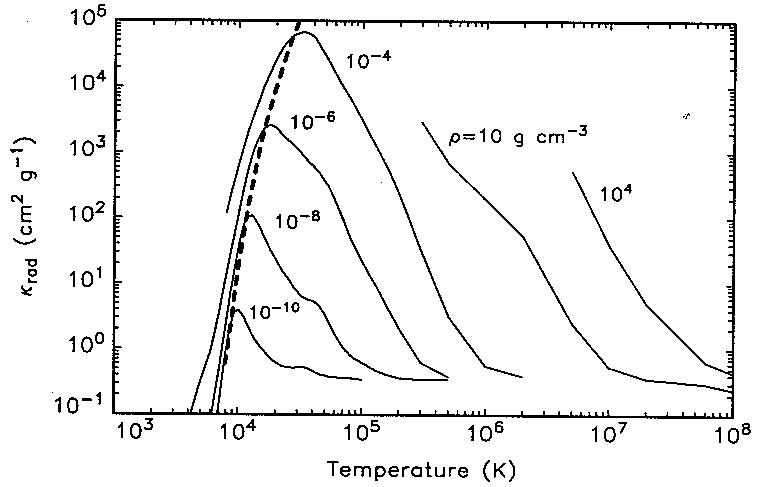
\includegraphics{stars_opacities}
      \caption{The radiative opacity as a function of temperature and density in a typical star.
               This plot is taken from HKT pg 217.}
      \label{fig:opacities}
      \end{figure}

      \newthought{At low temperatures,} (between about $10^3$ and $10^4$ K),
      the dominant form of continuous opacity is H$^-$ bound-free and free-free opacity.
      If there are enough free electrons present (easier with increased partial ionization of
      heavy elements), some will become weakly bound to hydrogen atoms, so that the proton is
      surrounded by two electrons. Opacity is caused by photoionization of this extra electron
      with binding energy of 0.75 eV (bound-free).
      Note that H$^-$ has only one energy level so there are no line transitions.

      \begin{equation}\boxed{
      \kappa_{H^{-}} \propto Z \rho^{1/2} T^{9}
      }\end{equation}
      
      The opacity is very sensitive to temperature, because a fragile balancing act is required.
      The temperature must be less than 10,000 K (when Hydrogen ionizes) so that neutral Hydrogen
      is around to get another electron. But, the temperature must also be high enough so that
      an abundance of free electrons are around which were liberated from ionized heavy elements.
      This opacity is also sensitive to metallicity, for the same reason. 
      Despite $H^{-}$ being a fragile and rare ion, this type of opacity is the most important
      source in our Sun's atmosphere, and is dominant in FGK stars\sidenote{
        Why can such a rare species dominate the opacity?  Recall, from chemistry class, that
        a negative anion \emph{always} has a larger radius than a positive cation.  The additional
        electron that the H$^-$ ion carries is very loosely bound, and so each H$^-$ ion is
        essentially a large puffy ball. Furthermore, any optical photon that hits this puffy
        ball will have enough energy to ionize the H$^-$ ion.
      }.

      \newthought{At slightly higher temperatures,} (between about $10^4$ and $10^7$ K, where
      the lower and upper limits are density dependent --
      see Figure~\ref{fig:opacities}) the opacity associated with transitions in
      neutral hydrogen become important.
      These include bound-bound transitions and bound-free transitions.
      
      In bound-bound 
      transitions, a photon is absorbed by an atom, moving an electron to a higher energy level.  
      These transitions have corresponding wavelengths associated with them, giving rise 
      to spectral lines.  Higher density leads to higher opacity, but the temperature 
      dependence of this opacity is complicated.  The temperature and composition determine 
      how many atoms of a certain type there are, and what state these atoms are in.  This 
      determines the strengths of spectral lines.  Of course, if the star is hot enough to 
      ionize everything, neutral transitions will not take place.
      
      Bound-free opacity is the ionization of an atom (H is most important, since it's most 
      abundant).  For photons with enough energy to ionize H, the cross section depends varies 
      as $\lambda^3$.  On our stars midterm, we had to plot bound-free opacity as a function of 
      wavelength.  I can't draw it here, but it's good to know what the plot looks like.  
      Bound-free opacity is responsible for the Balmer jump in stellar spectra at 365 nm, where 
      H in the $n=2$ level can be ionized.  This produces a drop in flux from the star at shorter 
      wavelengths.

      Averaging bound-free and free-free absorption over all wavelengths gives Kramer's opacity:
      \begin{equation}\boxed{
      \bar{\kappa}\propto \frac{\rho}{T^{3.5}}
      }\end{equation}
       
      \newthought{Once the temperature is} high enough such that all species are ionized,
      the dominant opacity source is electron scattering (Thomson scattering).
      This opacity is generally close to constant, since the Thomson cross-section is a constant given by
      (see Section~\ref{sec:thomson})
      \begin{equation}
      \sigma_{\rm T} = \frac{8 \pi e^4}{3 c^4 m_e^2} = 6.6524\times 10^{-25}~{\rm cm}^2\,\, .
      \end{equation}
      The opacity $\kappa = \sigma / m$, so the opacity will depend on the total mass per
      scattering electron; that is, it will depend on the composition of the material and also
      how much it is ionized. Because of the ionization state, it will also depend on the
      temperature, i.e. whether the material is fully ionized. For a fully ionized medium,
      however, the opacity should be roughly constant, since there will typically be 1 or 2
      baryons per electron, so $m \sim 1-2~m_p$. Therefore $\kappa$ is usually of the order
      0.1-0.4 cm$^2$ g$^{-1}$.

      The exact opacity (assuming a fully ionized gas) from Thomson scattering can be calculated 
      as a function of H mass fraction.  In a similar calculation to the mean molecular weight 
      derivation, 
      \begin{equation}
      n_e=n_H+2n_{He}+\Sigma{A}{2}n_A=\frac{\rho}{m_H}\left(X+\frac{2}{4}Y+\frac{1}{2}Z\right)=\frac{\rho}{2m_H}\left(1+X\right)
      \end{equation}
      So,
      \begin{equation}\boxed{
      \kappa_T=\frac{n_e\sigma_T}{\rho}=\frac{\sigma_T}{2m_H}\left(1+X\right)=\left(1+X\right)0.2~{\rm cm^2 g^-1}
      }\end{equation}
\end{enumerate}

\subsection{Stellar Properties}
Let's start by listing the properties of the Sun, which are just good to know.
\begin{dgroup}
\begin{dmath}
L_\astrosun = 3.8 \times 10^{33}~{\rm erg}~{\rm s}^-1
\end{dmath}
\begin{dmath}
R_\astrosun = 6.9 \times 10^{10}~{\rm cm}
\end{dmath}
\begin{dmath}
M_\astrosun = 2 \times 10^{33}~{\rm g}
\end{dmath}
\begin{dmath}
t_\astrosun = 4.5 \times 10^9~{\rm yrs}
\end{dmath}
\begin{dmath}
T_{\rm eff} = 5800~{\rm K}
\end{dmath}
\begin{dmath}
T_{\rm c} = 15 \times 10^6~{\rm K}
\end{dmath}
\begin{dmath}
\rho_{\rm c} = 150~{\rm g}~{\rm cm}^{-3}
\end{dmath}
\begin{dmath}
\langle \rho \rangle_\astrosun = 1~{\rm g}~{\rm cm}^{-3}
\end{dmath}
\end{dgroup}
Ranges for other stars:
\begin{dgroup}
\begin{dmath}
M \sim 0.1 - 100~{\rm M}_\astrosun
\end{dmath}
\begin{dmath}
R \sim 0.1 - 1000~{\rm R}_\astrosun
\end{dmath}
\begin{dmath}
L \sim 10^{-4} - 10^6~{\rm L}_\astrosun
\end{dmath}
\begin{dmath}
T_{\rm eff} \sim 1000 - 5 \times 10^4~{\rm K}
\end{dmath}
\end{dgroup}

\subsection{Spectral Types}
O, B, A, F, G, K, M\newline
Within these types, stars are numbered 0 through 9 (hottest to coolest).  Luminosity classes 
are also used.  I-IV are giant stars, while V are main sequence stars.  D is for white dwarfs.  
So, for example, the Sun is a G2V star.\newline
O stars:\newline
>16 $M_{\odot}$, $M_V=-5$ or brighter\newline
Very weak spectral lines (just about everything is ionized, so there's nothing 
to produce transitions).  Very weak Balmer lines and some weak lines to due 
ionization of He.  No Balmer break visible.\newline
B stars:\newline
2-16 $M_{\odot}$\newline
Stronger Balmer lines, also He absorption lines.  Still a relatively clean 
spectrum though.  Balmer break visible (and visible in all later spectral 
types.\newline
A stars:\newline
1.5-2 $M_{\odot}$, $M_V\sim 0$\newline
Strongest Balmer lines because these are the hottest stars (hot enough to have 
lots of H in the n=2 state) without being too hot and ionizing all the H.  
Effective temperature of $\sim$10,000 K is perfect for Balmer lines.\newline
F stars:\newline
1-1.5 $M_{\odot}$\newline
Balmer lines start to weaken again.  Star seeing metal lines (mainly neutral 
or singly ionized Ca, Mg, and Na).\newline
G stars:\newline
0.8-1 $M_{\odot}$, $M_V\sim4$\newline
This includes the Sun.  Weaker Balmer lines, stronger metal lines.\newline
K stars:\newline
0.5-0.8 $M_{\odot}$\newline
Weaker Balmer, stronger metal.  Also start seeing absorption bands from 
molecules (smearing of lots of absorption lines due to rotational, vibrational, 
and electronic transitions).
M stars:\newline
<0.5 $M_{\odot}$, $M_V\sim 8-12$\newline
Dominated by molecular bands, in particular TiO between 6600\AA\ and 8600\AA.

\subsection{HR Diagram}
Be able to draw and explain one.  Some useful approximate relations for the main sequence:
\begin{equation}L\propto T_{eff}^8\end{equation}
\begin{equation}R\propto T_{eff}^2\end{equation}
\begin{equation}L\propto M^3\ for\ stars\ more\ massive\ than\ the\ Sun\end{equation}
\begin{equation}L\propto M^5\ for\ stars\ less\ massive\ than\ the\ Sun\end{equation}
Main sequence masses range from $\sim 0.1\ M_{\odot}$ to $\sim 100\ M_{\odot}$.  Main sequence 
radii range from $\sim 0.25\ R_{\odot}$ to $\sim 25\ R_{\odot}$.  Temperatures range from 
around $2000-3000\ K$ to $\sim 50,000\ K$.  Luminosities range from $\sim10^{-3}L_{\odot}$ to 
$\sim500,000-1,000,000L_{\odot}$ (somebody should check these ranges, they're estimates/pulled 
from Wikipedia).  

Since the energy of a star comes from its mass, main sequence lifetimes can be estimated as
\begin{displaymath}
\tau_{ms}\sim\frac{E}{L}\sim\frac{M}{L}\sim M^{1-\alpha}
\end{displaymath}
where $\alpha$ is given by the mass-luminosity relation.  So, for stars more massive than the 
Sun,
\begin{equation}
\tau_{ms}\sim M^{-2}
\end{equation}
and for stars less massive than the Sun,
\begin{equation}
\tau_{ms}\sim M^{-4}
\end{equation}
Anything less massive than the Sun basically lives forever.

\subsection{Equations of Stellar Structure}
\newthought{There are three} key pieces of physics that are necessary for understanding stars:
\begin{enumerate}
    \item Force balance: pressure vs. gravity (and sometimes rotation)
    \item Energy transport: conduction, radiation, convection
    \item Energy generation: fusion, gravitational contraction
\end{enumerate}
These form the essence of the equations of stellar structure.
\begin{dgroup*}
\begin{dmath}
    \frac{\d M_r}{\d r} = 4\pi r^2\rho \quad \text{(mass continuity)}
\end{dmath}
\begin{dmath}
    \frac{\d P}{\d r} = -\frac{GM_r\rho}{r^2} \quad \text{(hydrostatic equilibrium)}
\end{dmath}
\end{dgroup*}

Let's talk first about force balance. Assuming no radiation, this is just a competition between pressure and gravity. We can look at a layer in the star with pressure $P$ at its base and $P+dP$ above, and we know the force on the layer due to gravity. The total force will be the pressure difference times the area of the shell $A$ (which will eventually drop out) plus the gravitational force $-\frac{G M_r M_{\rm shell}}{r^2}$. If we assume hydrostatic equilibrium, the total force is zero. We then can switch to differentials to get the hydrostatic equilibrium equation:

\begin{equation}
\frac{dP}{dr} = -\frac{\rho G M_r}{r^2}\,\,.
\end{equation}

The mass continuity equatin just comes from the amount of mass in a spherical shell at radius r 
and of thickness dr.

The radiative temperature gradient can be derived by considering the energy in shells at different 
radii.  Since energy flows out of the star, the energy density must decrease outwards.  Consider 
a shell with energy denstity $u+du$ (shell 1), with another shell $dr$ above it of energy 
density $u$ (shell 2).  The energy flow from shell 1 to shell 2 per unit time ($L(r)$) is 
the excess energy in shell 1 divided by the time it takes for this energy to flow from shell 1 to 
shell 2.  So
\begin{equation}\label{eq:L}
L(r)=-\frac{4\pi r^2\,dr\,du}{(dr)^2/lc}
\end{equation}
where the denominator is the time it takes a the photon to cross from shell 1 to shell 2 by random 
walk.  Taking the angle of the radiation into account introduces a factor of 1/3 on the right hand 
side.  Equation \ref{eq:L} can be rewritten as 
\begin{equation}
\frac{L(r)}{4\pi r^2}=-\frac{cl}{3}\frac{du}{dr}
\end{equation}
This can also be thought of as a diffusoin equation, where the left hand side is energy flux, 
$\frac{cl}{3}$ is the diffusion coefficient, and $\frac{du}{dr}$ is the energy density gradient.  
Plugging in $u=aT^4$ and $l=\frac{1}{\kappa\rho}$, and solving for $\frac{dT}{dr}$ gives
\begin{equation}\label{eq:rad}
\boxed{\frac{dT(r)}{dr}=-\frac{3L(r)\kappa(r)\rho(r)}{4\pi r^2 4acT^3(r)}}
\end{equation}

The energy conservation equation just comes from defining $\epsilon(r)$ as the power generated 
per unit mass.  With this definition,
\begin{equation}
\boxed{\frac{dL(r)}{dr}=4\pi r^2\rho (r)\epsilon (r)}
\end{equation}

In addition to the four main equations of stellar structure, three more equations must be 
specified for the pressure, opacity, and energy generation.  
\begin{equation}
P=P(\rho,T,composition)
\end{equation}
\begin{equation}
\kappa=\kappa(\rho,T,composition)
\end{equation}
\begin{equation}
\epsilon=\epsilon(\rho,T,composition)
\end{equation}
Also, the four differential equations require four boundary conditions:
\begin{equation}
M(r=0)=0
\end{equation}
\begin{equation}
L(r=0)=0
\end{equation}
\begin{equation}
P(r=R)=0
\end{equation}
\begin{equation}
M(r=R)=M_*
\end{equation}

So, there are 7 equations for 7 unknowns, and 4 boundary conditions for 4 differential equations.  
This means that there is a unique solution given the composition and total mass of the star, the 
only two free parameters in the equations.  This is the \emph{Vogt-Russell conjecture}, that the 
properties and evolution of a star depend only on its mass and initial composition.

The equation of state is almost always ideal gas, but here's a good derivation of mean molecular 
weight, which I personally can never remember.

For a fully ionized gas, H contributes 2 particles, He contributes 3, and metals contribue 
$\sim\frac{A}{2}$.  So the total number density of particles is
\begin{equation}
n=2n_H+3n_{He}+\Sigma \frac{A}{2}n_A=\frac{rho}{m_H}\left(2X+\frac{3}{4}Y+\frac{1}{2}Z\right)=\frac{\rho}{2m_H}\left(3X+\frac{1}{2}Y+1\right)
\end{equation}
using the fact that $X+Y+Z=1$.  Then
\begin{equation}
\mu=\frac{\rho}{nm_H}=\frac{2}{1+3X+0.5Y}
\end{equation}

io likes the following definition of mean molecular weight:
\begin{equation}
\frac{1}{\mu_I} = \sum \frac{X_i}{A_i}\,\, ,
\end{equation}
\begin{equation}
\frac{1}{\mu_e} = \sum \frac{Z_iX_i}{A_i} \,\, ,
\end{equation}
\begin{equation}
\frac{1}{\mu} = \biggl(\frac{1}{\mu_I} + \frac{1}{\mu_e} \biggr)^{-1}\,\,.
\end{equation}

See the will ask question for a discussion of opacity.

Also, radiation pressure can contribute to the overall pressure (and sometimes dominate).  
For a photon gas,
\begin{equation}
P_{rad}=\frac{1}{3}u=\frac{1}{3}aT^4
\end{equation}

\subsection{The Hayashi Track}\label{sec:hayashi}
\newthought{The Hayashi track}
describes the evolution of star that is entirely convective
(with a narrow radiative envelope for the photosphere).
Hayashi derived these tracks by showing that for
a given mass, there is an effective temperature below which no stable solutions exist.
That is, any star with an effective temperature below the limit will collapse until its
effective temperature is above the limit.  In this way, stars essentially slide along
the boundary of stability, maintaining a constant effective temperature
(even as their central temperature increases).

Let's see a brief derivation of this.  To begin with we assume that the interior is entirely
convective so that the pressure is given by the adiabatic relationship
\begin{dmath}
    P\propto\rho^\gamma
\end{dmath},
By combining this with the ideal gas law, we find that
\begin{dmath}\label{eq:pt_adiabatic}
    P\propto T^{\frac{\gamma}{\gamma-1}}
\end{dmath}.
For a monatomic gas, $\gamma=5/3$, so that $P\sim T^{5/2}$.

Next we can use the equation of hydrostatic equilibrium to estimate the central pressure $P_c$ and
temperature $T_c$ as\sidenote{
    To see this, approximate $\d P/\d r$ as $P_c/R$ and approximate $\rho$ as $M/R^3$.
    Forget about numerical constants because we're just looking for a scaling relationship
    here.  The temperature comes from the ideal gas law.
}:
\begin{dgroup*}
\begin{dmath*}
    P_c \sim \frac{M^2}{R^4}
\end{dmath*}
\begin{dmath*}
    T_c \sim \frac{M}{R}
\end{dmath*}
\end{dgroup*}
With these expressions for the central pressure and temperature, we can use
Equation~\ref{eq:pt_adiabatic} to find the pressure and temperature anywhere in the
star -- notably at the surface of the photosphere.

However, before we can do that, we need to locate the photosphere.  To do this, we
assume an opacity law of the form $\kappa \sim \rho T^a$, and that the photosphere
can be treated in the plane-parallel approximation\sidenote{
    This assumes that the photosphere is narrow and contains a negligible amount of mass.
}.
In this case the equation of hydrostatic equilibrium becomes
\begin{dmath*}
\frac{\d P}{\d z} = -\rho g
\end{dmath*},
where $g = GM/R^2$.  The photosphere is located where $\tau\sim 1$ (or $\tau\sim 2/3$ if
you're being picky), so let's replace $\d z$ with the optical depth $\d\tau = -\kappa\rho\d z$
such that
\begin{dmath*}
\frac{\d P}{\d\tau} = \frac{g}{\kappa}
\end{dmath*}.
Integrating to the surface of the photosphere therefore gives us
\begin{dmath}
    P_{\rm eff} \sim \frac{g}{\kappa} \nolinebreak
                \sim \frac{R}{T_{\rm eff}^a}
\end{dmath}.
Using Equation~\ref{eq:pt_adiabatic} and our expressions for $P_c$, $T_c$, and $P_{\rm eff}$
we can solve for $T_{\rm eff}$ to find (taking $\gamma=5/3$)
\begin{dmath}\boxed{
    T_{\rm eff} \sim R^{2.5/(2.5+a)}M^{0.5/(2.5+a)}
}\end{dmath}.
Therefore when the opacity is very temperature sensitive\sidenote{
    For H$^-$ opacity, $a\sim10$.
}, the effective temperature is almost independent of radius.  Therefore the Hayashi
track is a vertical line on the HR diagram.

It is worth noting here that it is critical for the opacity to increase rapidly with temperature.
As the star contracts, the central temperature of the star increases.  In fact, at any fixed
position within the star, the temperature increases.  However, if the opacity is very temperature
sensitive, the photosphere will stay at a location where the temperature remains roughly
constant.  This means that the effective temperature stays constant.

\subsection{The Henyey Track}

\newthought{In the core}
of a protostar, Kramer's opacity law is a good description of the mean opacity.
As the protostar contracts along the Hayashi track, the temperature of the core increases
even as the effective temperature remains constant.  The opacity in the core therefore decreases
as the star contracts and eventually the core becomes radiative.  As the star continues to
contract, the opacity in the core further decreases and the radiative region grows in size.
Therefore the structure of the star responds to further contraction by lowering the opacity
in its core and moving more energy through radiation.  This allows the star to push more energy
out (it's more transparent to radiation!), and hence the luminosity increases.  Because the
luminosity is increasing while the radius is shrinking, the effective temperature must also
increase (it can no longer remain constant as on the Hayashi track)\sidenote{
    Recall that $L=4\pi R^2\sigma T_{\rm eff}^4$ to good approximation.
}.  Therefore, when the core becomes radiative, the protostar moves to higher luminosities and
higher effective temperatures (after moving to lower luminosities with a constant effective
temperature on the Hayashi track).  This track is occasionally called the Henyey track.

\indent The relation between luminosity, mass, and T$_{eff}$ for objects on the Henyey track can be derived with homology, using the following scaling relations which apply to the core of the protostar:

\begin{enumerate}
	\item Kramer's opacity: $\kappa \propto \rho T_{c}^{-3.5}$
	\item Ideal gas: $P \propto \rho T_{c}$, where $\rho \propto M R^{-3}$
	\item Radiative energy transport\sidenote{This scaling relation comes from solving for $\kappa$ in Equation \ref{eq:rad}, and approximating $dT(r)/dr$ as $T/R$}: $\kappa \propto T_{c}^{4} L^{-1} M^{-1} R^{4}$
\end{enumerate}

\noindent Finally, by using everyone's favorite $L \propto R^{2} T_{eff}^{4}$, you find that

\begin{equation}
L \propto M^{22/5} T_{eff}^{4/5}
\end{equation}

This equation illustrates what was described above -- as the core becomes radiative, an increase in $L$ corresponds to an increase in $T_{eff}$.

\newthought{Cool note} on the Henyey Track -- if the mass of the protostar is too low, then hydrogen burning ignites before the events which cause the protostar to travel along the Henyey track can begin.  Thus, the resulting main sequence star will remain completely convective -- this is why main sequence stars with mass $< .8 M_{\odot}$ are fully convective (and why their Hayashi tracks directly intersect the main sequence, without the upward trend of the Henyey track; see Figure 2.2 in HKT for a good plot illustrating this).  

\subsection{Scaling Relations on the Main Sequence}
Assume that P(r), M(r), $\rho (r)$, and T(r) are roughly power laws.  Then from the equations of stellar structure we have:

\begin{equation}
P \thicksim \frac{\rho M}{r}
\end{equation}
\begin{equation}
M \thicksim r^3\rho
\end{equation}
\begin{equation}
L \thicksim \frac{T^4r}{\kappa \rho}
\end{equation}

For moderately massive stars greater than $1 M_\odot$, the pressure is dominated by kinetic gas pressure and the opacity is dominated by electron scattering.

\begin{equation}
P \thicksim \rho T
\end{equation}
\begin{equation}
\kappa = constant
\end{equation}

Equating hydrostatic equilibrium with the equation of state:

\begin{equation}
P \thicksim \frac{M\rho}{r} \thicksim \rho T
\end{equation}
\begin{equation}
T \thicksim \frac{M}{r}
\end{equation}

Replacing T in the luminosity equation yeidls:
\begin{equation}
L \thicksim M^3
\end{equation}

Furthermore, $M \thicksim R$ on the main sequence, which implies a constant core temperature.  To see this, consider a star that is contracting and heating up.  An equilibrium will be established when the density and the temperature in the core are high enough for the onset of nuclear reactions.  Since the nuclear power density $\epsilon$ depends mainly on temperature, for any initial mass, the radius of the star will stop shrinking when a particular core temperature is reached.  Therefore the internal temperature is comparable in all main sequence stars.  From stellar models, over a range of around 100 in mass, the core temperature varies only by a factor of 4.  

For stars less massive than the sun, the opacity is dominated by bound-bound and bound-free opacities, which follow kramer's opacity $\kappa \thicksim \rho T^{-3.5}$.  Since the temperature is approximately constant:

\begin{equation}
 M \thicksim R
\end{equation}
\begin{equation}
\kappa \thicksim \rho \thicksim \frac{M}{r^3} \thicksim M^{-2}
\end{equation}

The luminosity equation becomes:

\begin{equation}
L \thicksim \frac{M}{M^{-2}M^{-2}} \thicksim M^{5}
\end{equation}

For the most massive stars, radiation pressure dominates.  The equation of state then goes as $P \thicksim T^4$, and electron scattering opacity dominates.  The mass-luminosity relationship then goes as:

\begin{equation}
L \thicksim M
\end{equation}





\subsection{Stellar Evolution}

Collapse from a gas cloud:

The first important thing to know is the Jeans criterion. You can get here by considering a deviation from a system in hydrostatic equilibrium, which is described by the Virial Theorem:

\begin{equation}
2K + U = 0\,\, ,
\end{equation}
where we can approximate the kinetic and gravitational potential energies as

\begin{equation}
U \sim \frac{3 G M_{\rm c}^2}{5 R_{\rm c}}
\end{equation}
\begin{equation}
K = \frac{3}{2} N k_{\rm B} T = \frac{3 M_{\rm c} k_\rm B T}{\mu m_{\rm H}}
\end{equation}

You can assume a constant density for the cloud and find the minimum mass necessary to start collapse, $M_{\rm c} > M_{\rm J}$:

\begin{equation}
M_{\rm J} \approx \biggl( \frac{5 k_{\rm B}T}{G \mu m_{\rm H}}\biggr)^{3/2}\biggl( \frac{3}{4\pi\rho_0}\biggr)^{1/2}
\end{equation}

We can also express this criterion as $R_{\rm c} > R_{\rm J}$, where

\begin{equation}
R_{\rm J} \approx \biggl( \frac{15 k_{\rm B} T}{4 pi G \mu m_{\rm H} \rho_0} \biggr)^{1/2}
\end{equation}

Once the Jeans criterion is satisfied, the cloud basically collapses in freefall at the beginning. It is isothermal, optically thin, and radiates energy efficiently. The freefall time is

\begin{equation}
t_{\rm ff} = \biggl( \frac{3 \pi}{32 G \rho_0}\biggr)^{1/2} \sim \biggl( \frac{1}{G \rho_0}\biggr)^{1/2}
\end{equation}
The numerical factor is from the derivation in Carrol \& Ostlie; you can derive this by considering a particle on the outer edge of and object falling inward due to the gravitational force of all the interior mass.

Also note that fragmentation is an issue: that is, the Jeans mass changes as the density of the cloud goes up, and a natural consequence of this is that a smaller mass is required to collapse. Therefore, one large cloud (of, say, 50 solar masses) might collapse into $\sim 50$ solar-mass clouds.

What eventually stops fragmentation is that the cloud stops being isothermal. The cloud starts transporting more energy adiabatically rather than radiatively because it starts to become optically thick, and radiation does not transport energy out efficiently enough.

(There is some stuff about shocks produced by the outer layers of the cloud free-falling onto the nearly hydrostatic star, which powers it for a while. Not sure how much we need to know about this.)

To see that fragmentation must stop, use the fact that the collapse becomes 
adiabatic.  So
\begin{equation}
T\propto\rho^{\gamma-1}
\end{equation}
Plugging this into the Jeans mass expression gives
\begin{equation}
M_J\propto\rho^{(3\gamma-4)/2}
\end{equation}
For $\gamma=5/3$, this gives $M_J\propto\rho^{1/2}$, so the Jeans mass 
increases with increasing density, which stops fragmentation.

As a fragmented clump collapses, it must have a way of releasing the energy from the collapse, or 
the temperature and pressure will rise and stop the collapse.  At this stage, the excess energy 
goes into first dissociating H$_2$, then ionizing atomic H.  Once (almost) all the H has been 
ionized, the star must release its gravitational energy by radiating.  This slows the collapse, 
and a slowly contracting proto-star forms, with contraction governed by the Kelvin-Helmholtz 
timescale.  

Pre-Main-Sequence Evolution:

First, the \textbf{pre-MS protostar} collapses on the Kelvin-Helmholtz timescale $t_{\rm KH}$, which for $1~{\rm M}_\astrosun$ is about $10^7$ years. The Kelvin-Helmoholtz timescale is given by
\begin{equation}
t_{\rm KH} \approx \frac{GM^2}{RL}\,\, .
\end{equation}
This just comes from approximating the energy available for the luminosity is the gravitational potential energy, so the timescale for radiating this energy is just the total gravitational potential energy divided by the luminosity.

The effective temperature increases, so the opacity of the outer layers becomes dominated by the H$^-$ ion, which gets its extra electrons from increased partial ionization of heavy elements. This increased opacity causes the envelope of the protostar to become convective and sometimes this envelope can become very large, reaching even to the center of the star. This object evolves along the Hayashi track, its luminosity decreasing while the effective temperature increases only slightly (it is almost constant, $\sim 3800$ K).

A \textbf{solar mass star on the Hayashi track} is completely convective and starts burning deuterium in the first million years, which slows the collapse slightly and for a short time, since deuterium is not very abundant. The central temperature rises, and opacity in the center decreases, so the core becomes radiative. This causes the luminosity to start increasing. At the same time, the core becomes hot enough to start more nuclear reactions (dominated by the first two steps of the PP chain and the CNO cycle. Nuclear energy generation starts dominating over luminosity from gravitational collapse. A large temperature gradient develops in the core, which starts to become partly convective again, and then the core expands a bit, which decreases the luminosity because $\epsilon_{\rm grav}$ becomes negative, and $\epsilon = \epsilon_{\rm nuc} + \epsilon_{\rm grav}$. When C-12 is exhausted, the core adjusts and PP-I chain dominates, and the star settles onto the main sequence.

For \textbf{lower-mass stars}, the temperature might never get hot enough to burn C-12, so they don't turn up as much in luminosity, but rather fall closer to the Hayashi track down onto the Main Sequence. Below about 0.08 M$_\odot$, no nuclear reactions can be sustained, and these stars never reach the Main Sequence. Lower mass starts also never develop radiative cores, so they are always fully convective.

\textbf{Massive stars} start burning carbon and hydrogen much more quickly because the central temperature rises faster. These break away from the Hayashi track earlier and at higher luminosities, since nuclear reactions contribute more to the luminosity earlier on. The CNO cycle becomes the dominant energy generation process because of the high temperatures. As the star travels horizontally on the HR diagram, the core remains convective because the energy generation is so temperature-dependent, while the envelope is radiative.

Main Sequence Evolution:

Low mass stars (the mass of the Sun or smaller) increase slightly in luminosity and temperature 
during their main sequence lifetimes.  This is due to the conversion of H to He in the core, 
increasing the mean molecular weight.  This reduces the pressure in the core (ideal gas law), 
causing the core to contract.  The gravitational energy released heats the surrounding material, 
allowing the H burning region to include more material.  Also, the increased temperature and 
density increases the rate of the pp chain.  As a result, the energy output of the core increases, 
increasing the overall luminosity of the star.  The energy released in contraction also goes 
into increasing the effective temperature.  This process causes the star to move up and to the 
left in the HR diagram.  As the H in the core of the star is depleted, an 
inert He core forms, with H shell burning around it.  This shell burning increases the luminosity 
of the star further, and also expands the outer layers, cooling the star.  The star now moves 
up and to the right in the HR diagram.  In stars more massive than the Sun, a convective 
core prevents this process from happening, as new material is brought into the burning region and 
He is removed.  As the star evolves, the convection in the core decreases and there is some 
buildup of He, although not as much as in lower mass stars.  

In high and low mass stars, main sequence evolution ends when too much He builds up in the core.  
The He core is isothermal and does not generate energy, so it must support itself with a density 
gradient.  Once the core reaches around 10\% the mass of the entire star, it will no longer 
be able to support itself or the material above it (note- in very low mass stars, electron 
degeneracy may set in before this happens.  I'm guessing this is how a He white dwarf would form). 
In higher mass stars, when star runs out of H, the entire star contracts, releasing graviational 
energy.  This increases luminosity, while the decrease in radius increases effective temperature.  

Post-Main Sequence Evolution:

This section makes a lot more sense with an HR diagram to refer too, so I'll be referring to the 
figures on page 458 and 459 of Carroll and Ostlie.  Solar mass and intermediate mass stars 
evolve similarly after the main sequence, although the shapes of their tracks are slightly 
different.  At this point, the star has an isothermal He core with H shell burning around it.  
The first stage in post-MS evolution is the \emph{subgiant branch}.  When the He core 
can no longer support itself, it contracts on a Kelvin-Helmholtz timescale, releasing energy and 
increasing luminosity.  The envelope of the star expands, lowering the effective temperature, and 
the star moves up and to the right on the HR diagram (labeled SGB).  As the star's envelope 
expands and cools, the opacity increases due to H$^-$.  This causes a convection zone to form, 
extended from surface of the star to most of the interior.  This convection transport energy from 
the interior to the surface more efficienty, causing a rapid increase in luminosity as the moves 
up the \emph{red giant branch} (RGB).  The path of the RGB is essentially the Hayashi track in 
reverse, which makes sense because both tracks deal with fully convective objects.  During this 
phase, convection brings products of nuclear burning such as C and N from the interior to the 
surface, where they can be seen spectroscopically (dredge-up).  This provides a test for stellar 
evolution models.  When a star reaches the tip of the RGB, the center becomes hot enough to begin 
fusing He through triple-$\alpha$.  The ignition of He expands the core and pushes the H burning 
shell outwards, cooling it and decreasing the rate of energy production.  Shell burning still 
supplies most of the star's luminosity, so the luminosity decreases rapidly (the dotted line on 
page 458).  The envelope of the star contracts during this process, causing the effective 
temperature to rise.   

In stars below $1.8\ M_{\odot}$, the ingition of He creates a \emph{He core flash}.  Before 
ignition starts, the He core is already degenerate.  Once He ignition happens, the energy released 
goes into lifting the degeneracy pressure, instead of expanding and cooling the core.  This leads 
to explosive He burning in the core, producing $10^{11}$ L$_{\odot}$ for a few seconds.  Most of 
this energy is absorbed by the outer layers of the star, so the luminosity on the HR diagram is 
not affected.  

The next step in post-main sequence evolution is the \emph{horizontal branch}.  The H burning 
shell continues to contract, with the increase in density causing an increase in energy output.  
This increases the effective temperature of the star, and the stars moves horizontally to the left 
on basically a He burning main sequence.  What follows is analogous to the subgiant and red giant 
branches.  The mean molecular weight in the He burning core increases, causing it to contract.  
The evelope expands and cools, moving the star to the right on the HR diagram.  As the 
H burning shell expands and cools, it turns off, leaving He burning to power the star.  
When the He in the core runs out, a He burning shell forms and the star moves up the 
\emph{asymptotic giant branch} (AGB).  It becomes convective and there is a second dredge-up 
phase.  Near the top of the AGB, the H burning shell re-ignites and dominates the stars 
luminosity.  The H burning shell begins dumping He onto the He burning layer, increasing its mass 
and making it degenerate.  This leads to periodic He flashes in the shell, which push out the 
H burning layer, cooling it and turning it off.  The luminosity of the star drops until the H 
shell re-ignites, and the process repeats.  Mass loss from the star during this phase can 
reach $10^{-4} M_{\odot}$ per year, due to the pulsations and the formation of high opacity dust 
grains in the cool, loosely bound outer layers of the star.  This forms an optically thick cloud 
of material around the star.  As this cloud continues to expand, it eventually becomes optically 
thin, and the hot core of the star is exposed.  This causes the observed effective temperature 
to increase, moving the star into the \emph{post-AGB} phase.  The expelled envelope becomes a 
planetary nebula and the core becomes a white dwarf, moving down the HR diagram onto the white 
dwarf sequence.  

So, as a quick summary of all this, the basic picture is a star's H runs out, the core 
contracts and the envelope expands as a H burning shell forms.  The star gets brighter and cooler, 
moving to the right and up.  The star becomes convective and moves up a vertical, Hayashi-like 
track.  Then the star starts burning He and settles onto a He main sequence until the He runs out 
and a He burning shell forms.  The core contracts, the envelope expands, and the star gets brighter 
and cooler, moving to the right and up.  The star becomes convective again and Hayashis (that 
should totally be a verb) vertically.  Finally, it blows off it's outer layers and the core 
becomes a C+O white dwarf.

I couldn't find a detailed section on post-MS evolution for massive stars, but I assume it's 
basically the same, just with additional burning stages all the way up to burning Si into Fe, 
which each stage happening faster.

\subsection{The Instability Strip}
The instability strip is a narrow temperature range (around $6000$ or $7000$ K) 
extending from horizontal branch high mass stars all the way down to the white 
dwarf sequence (see Figure \ref{fig:strip}.  Stars in the instability strip 
undergo radial pulsations that change their temperature and luminosity.  
The pulsations are caused by the location of the HeII partial ionization 
zone in these stars.  At temperatures of $\sim40,000$ K, HeII will be partially 
ionized into HeIII.  The process of ionizing HeII creates a high Kramers' 
opacity in these regions, trapping energy and compressing the gas (I'm 
guessing from radiation pressure?).  Kramers' opacity goes as 
$\kappa\propto\rho/T^{3.5}$, so normally when gas in a star is compressed, the 
opacity decreases because the temperature rises.  In the HeII partial 
ionization zone, however, most of the trapped energy goes into further 
ionization, and the temperature does not increase much.  The increase in 
density then raises the opacity even more, and the layer is pushed outwards 
by radiation pressure.  As the layer rises, it expands, but does not cool 
much because recombination occurs instead.  This can be thought of as a 
``phase change'' in the gas.  Changes in energy go into changing the ionization 
state of the gas, instead of changing the temperature.  The decrease in 
density decreases the opacity, and the layer sinks back down, starting the 
process over again.  This is known as the $\kappa$ mechanism.  This 
process can also take place in zones of partially ionized HeI and HI, but 
simulations show the HeII zone is most important.  

\begin{figure}[ht]
\centering
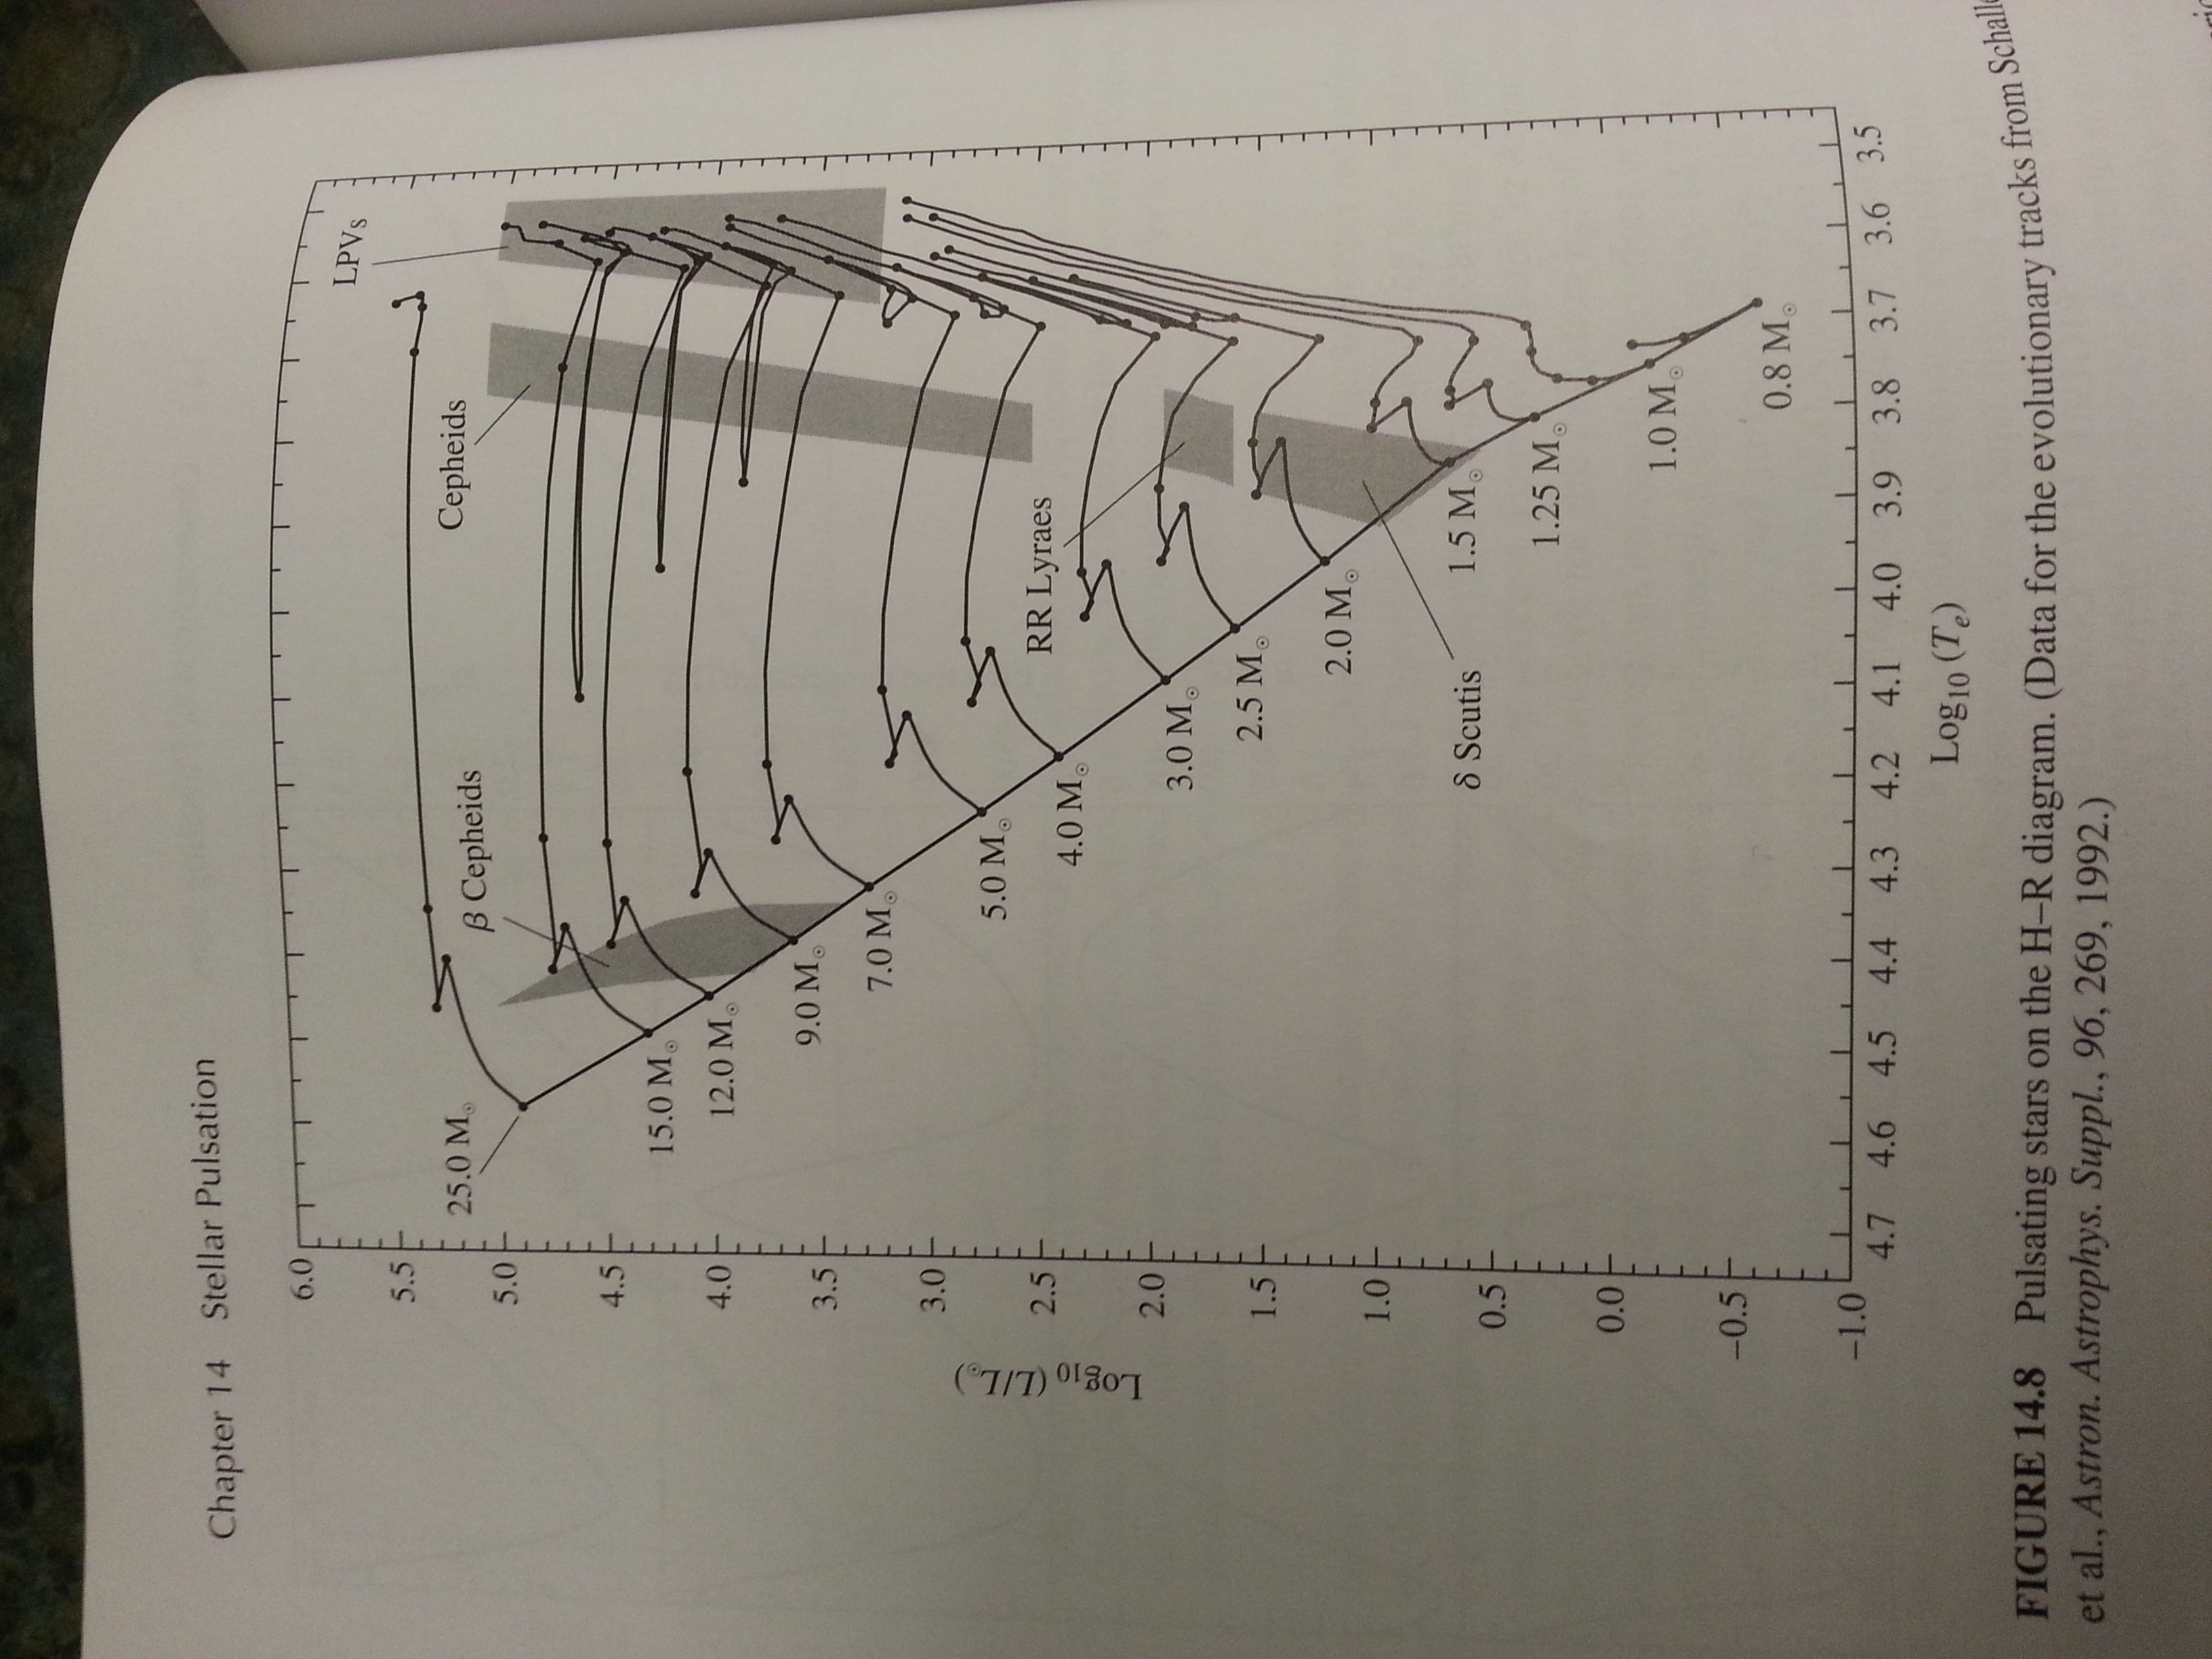
\includegraphics[width=\textwidth, angle=270]{strip.jpg}
\caption{The Instability Strip \label{fig:strip}}
\end{figure}


This process can take place in any star, but the reason surface pulsations 
are only observed in a narrow strip has to do with the depth of the HeII 
zone in the star.  If the star is hotter than around $7500$ K, the zone 
will be too close to the surface, where the low density means there is not 
enough mass to drive oscillations.  If the star is cooler than around $5500$ K, 
convection in the atmosphere will damp $\kappa$ mechanism oscillations.  
Important pulsating stars are Cepheids (high mass evolved stars, periods 
of days to $10$s of days, used as distance indicators), RR Lyraes (intermediate 
mass evolved stars, periods of a few hours to a day, used to find distances 
to globular clusters), $\delta$ Scutis (main sequence or just off main sequence 
A and F stars, periods of a few hours), and ZZ Cetis (white dwarfs, periods 
of less than an hour). 

\subsection{Radial Velocities}

Derivation of radial velocity amplitude from a star and a low mass companion (say a planet).

Let $r_p$ be the distance between the planet and the center of mass of the system, and $r_s$ be the distance between the star and the center of mass.

\begin{equation}
a = r_p + r_s
\end{equation}

\begin{equation}
v_p = \frac{2\pi r_p}{P}
\end{equation}
\begin{equation}
v_s = \frac{2\pi r_s}{P}
\end{equation}

\begin{equation}
M_pr_p = M_sr_s
\end{equation}

Combining above equations yields the following relation:
\begin{equation}
\frac{v_p}{v_s} = \frac{r_p}{r_s} = \frac{M_s}{M_p}
\end{equation} 

\begin{equation}
a = r_p + r_s = (\frac{M_s}{M_p} + 1)r_s = r_s\big(\frac{M_s + M_p}{M_s}\big)
\end{equation}

Plugging the above expression into Kepler's 3rd law:

\begin{equation}
P^2 = \frac{4\pi^2r_s^3(M_p + M_s)^2}{GM_p^3}
\end{equation}

Plugging in for $r_s$ and rearranging a bit:

\begin{equation}
v_s^3 = \frac{P^{-1}2\pi GM_p^3}{(M_p + M_s)}
\end{equation}

By assuming the companion is significantly less massive than the star, you can simplify the expression for the radial velocity amplitude K.  
\begin{equation}
v_s = K = 2\pi G P^{-\frac{1}{3}}M_pM_s^{-\frac{2}{3}}
\end{equation}

\subsection{Atmospheres}
The Boltzmann and Saha equations are probably more involved than we need to know (especially the 
Saha equation), but here they are anyway.
\begin{equation}
\frac{n_1}{n_2}=\frac{g_1}{g_2}e^{-(E_1-E_2)/kT}
\end{equation}
\begin{equation}
\frac{n_{i+1}}{n_i}=\frac{2Z_{i+1}}{n_eZ_i}\left(\frac{2\pi m_ekT}{h^2}\right)^{3/2}e^{-\chi_i/kT}
\end{equation}
where $n_{i+1}$ and $n_i$ are are the numbers of atoms in the $i$ or $i+1$ ionization state, 
$Z_i$ is the partition function of the $ith$ ionization state, and $\chi_i$ is the ionization 
energy.  All we should probably know for these equations relating to stars is that the describe 
the population of atoms in the star's atmosphere, and thus determine the strengths of spectral 
lines.  For example, the competing temperature dependence of these equations gives that the 
peak fraction of H atoms in the $n=2$ state happens at around 10,000 K.  This is why A stars show 
such strong Balmer lines.

Optical Depth and the atmosphere:
Using the radiative transfer equation with simplifying assumptions (plane-parallel atmosphere, 
wavelength independent opacity (grey), and the Eddinton approximation- the intensity of radiation 
is just an average of outward and inward radiation), can show that (see Carroll and Ostlie pg 
258-263) the temperature in the 
atmosphere varies with optical depth as:
\begin{equation}
T^4=\frac{3}{4}T_{eff}^4\left(\tau_{\nu}+\frac{2}{3}\right)
\end{equation}
This equation implies that the photosphere (where $T=T_{eff}$) is at $\tau=2/3$.  This also 
explains spectral lines and limb darkening.  If a certain wavelength corresponds to an atomic 
transition, that wavelength will have a higher opacity than the continuum.  So the point 
where $\tau=2/3$ will be higher in the star at that wavelength (in other words, you can't 
see as deep into the star at that wavelength).  Because of this, the light we see at that 
wavelength comes from cooler gas than light from the continuum, so there is less flux at that 
wavelength.  Limb darkening is the same idea.  At the edge of the disk of a star, we look into 
the atmosphere at an angle from the verticle direction, so $\tau=2/3$ is higher in the atmosphere, 
and thus cooler, so we see less flux from it.  In both cases, the effective temperature at 
$\tau=2/3$ is cooler.

Spectral Lines:
Spectral lines are broadened by natural broadening, Doppler broadening, and pressure broadening.  
Natural broadening is due to the uncertainty principle.  Since an electron spends a short time 
in an excited state, there is an uncertainty the energy of the state.  This makes the wavelenght 
of light that can be absorbed uncertain.  The typcial full-width-half-max of natural broadening is 
of the order of $10^{-5}nm$.  Doppler broadening is due to random thermal motions of the gas 
described by the Maxwell-Boltzmann distribution.  In the Sun, with $T_{eff}=5777 K$, the 
full-width-half-max of this effect is $\sim 10^{-2}$ nm.  Large-scale motions, such as turbulence, 
rotation, mass loss, and pulsation also contribute to Doppler broadening.  Doppler broadening 
is wider than natural broadening, but falls off exponentially, much faster than natural 
broadening (so the center line shape is due to Doppler broadening, but the wings are shaped by 
natural and pressure broadening.  Pressure broadening is caused when collisions of individual 
particles and electric fields of large numbers of particles perturb the energy levels of atoms.  
Pressure broadening has a similar shape and full-width-half-max to natural broadening.

\subsection{Interiors}
Most of this is covered in the stellar structure equations section.  The only other thing I can
think of is polytropes.  Maybe just some basic knowledge of them would be good (enough to 
answer that question Shri kept asking us in stars about what it means for white dwarfs or 
protostars to have a certain polytropic index).

\subsection{Homology}

Homology is used to find scaling relations between properties of a star, e.g. $R(M), L(M), P_{c}(M), T_{c}(M)$ to name a few.  We must first determine four things about the star we are considering:

\begin{enumerate}
	\item Is pressure given by ideal gas ($P \propto \rho T$) or radiative pressure support ($P \propto T^{4}$).
	\item Is the luminosity carried by radiative diffusion ($\kappa \propto T^{4} L^{-1} M^{-1} R^{4}$)\sidenote{This scaling relation comes from solving for $\kappa$ in Equation \ref{eq:rad}.} or convection ($T \propto M R^{-1}$)\sidenote{From the adiabatic temperature gradient, Equation \ref{conv}}.
	\item Is Thomson ($\kappa \propto \rho^{0} T^{0}$) or Kramer's opacity ($\kappa \propto \rho T^{-3.5}$) dominating.
	\item Through what process is fusion occurring, e.g. p-p chain ($\epsilon \propto \rho T^{4}$) or CNO cycle ($\epsilon \propto \rho T^{15}$).
\end{enumerate}

Then, using the equations of \textbf{mass continuity}

\begin{equation}
\rho \propto \frac{M}{R^{3}}
\end{equation}

\noindent and \textbf{hydrostatic equilibrium}

\begin{equation}
P \propto \frac{M \rho}{R}
\end{equation}

\noindent and the \textbf{energy conservation} equation

\begin{equation}
L \propto R^3 \rho \epsilon
\end{equation}

\noindent we can set up a system of equations to solve for whatever scaling relation we desire for the star.


\subsection{Nuclear Energy Generation}

Nuclear reactions are the primary power source in stars -- for stars on the main sequence, it is the fusion of four hydrogen nuclei into one $^{4}$He.  For fusion to occur, an atomic nucleus must overcome the Coulomb barrier of another nucleus into the potential well created by the strong nuclear force which binds nuclei together.

In the classical picture, the ability of a particle to overcome the Coulomb barrier is determined by whether the thermal energy is greater than the Coulomb potential energy.  The temperature $T_{classical}$ required to overcome the barrier can be estimated using the following equation\sidenote{This doesn't take into account the fact that the Maxwell-Boltzmann distribution of velocities will give some of the particles much higher velocities than $v_{avg}$ and therefore much higher thermal energies.  But this gives a good general picture of why we need quantum mechanics to describe nuclear reactions!}:

\begin{equation}
\frac{3}{2} k T_{classical} = \frac{Z_{1} Z_{2} e^2}{r}
\end{equation}

\begin{equation}
T_{classical} \sim 10^{10} \text{  K}
\end{equation}

\noindent assuming the collision is between two protons and $r$ is the radius of a typical nucleus ($10^{-10}$ cm).  Since the Sun's central temperature is on the order of $10^7$ K, there would not be a sufficient number of particles with high enough thermal energies to overcome the Coulomb barrier and thereby power the Sun.

The answer is (\textit{clearly}) quantum mechanical tunneling, whereby the inherent uncertainty in the position of the particle is large enough that even though there is not enough kinetic energy in the collision of two particles, one can still wind up in the potential well of the other and allow fusion to proceed.

The probability of successful tunneling (and a nuclear reaction occurring) is related to the ratio of the Coulomb barrier height to the initial kinetic energy of the incoming nucleus (this can be visualized by associating a \textit{larger} ratio with a \textit{wider} barrier and therefore a lower probability of tunneling -- see Figure 10.4 in Carroll and Ostlie).  Specifically, the probability for penetrating the Coulomb barrier is 

\begin{equation}
g(E) = e^{-\sqrt{E_{G}/E}}
\end{equation}

\noindent where $E$ is the particle kinetic energy and $E_{G}$ is the Gamow energy\sidenote{$\alpha=\frac{e^2}{\hbar c} = \frac{1}{137}$ is the fine structure constant and $\mu$ is the reduced mass.}:

\begin{equation}
E_{G} = \left(\pi \alpha Z_{1} Z_{2} \right)^2 2 \mu c^2
\end{equation}


The probability for a nuclear reaction, however, will depend not only on the probability of penetrating the Coulomb barrier, but on the nuclear cross section, which should scale as $1/E$.  The cross section is

\begin{equation}
\sigma(E) = \frac{S(E)}{E} g(E) =  \frac{S(E)}{E} e^{-\sqrt{E_{G}/E}}
\end{equation}

\noindent where $S(E)$ is some function which varies very slowly as a function of energy, so we can write it as a constant\sidenote{Sometimes, $S(E)$ does not hold constant, but peaks rapidly at specific energies that correspond to energy levels within the nucleus due to the resonance between the nucleus' energy level differences and the energy of the incoming particle.  This resonance phenomenon is important in the triple-alpha process.}.

The rate of nuclear reactions (number of reactions per time per volume) is given by 

\begin{equation}
R_{AB} = n_{A} n_{B} \sigma_{AB} v_{AB}.
\end{equation}

If the average energy per reaction $\Delta mc^2 = Q_{AB}$, then the energy generation (power per unit mass) is 

\begin{equation}\label{engen}
\epsilon = \frac{Q_{AB} R_{AB}}{\rho} = Q_{AB} \frac{n_{A} n_{B}}{\rho} \left<\sigma_{AB} v_{AB}\right>.
\end{equation}

We want to average $\sigma_{AB} v_{AB}$ over all velocities, where the distribution of velocities is given by the Maxwell-Boltzmann distribution\sidenote{Even though we're in the center of a star and the gas is really hot, the MB distribution still applies because our nuclei still constitute a classical, (nuclei are massive and slow) non-relativistic gas.}.  Therefore, we get that

\begin{equation}
\left< \sigma_{AB} v_{AB} \right> = \int_0^{\infty} \sigma_{AB} v_{AB} P(v_{AB}) dv_{AB}
\end{equation}

where

\begin{equation}
P(v)dv = 4 \pi \left( \frac{\mu}{2 \pi kT} \right)^{3/2} v^2 \exp\left(- \frac{\mu v^2}{2kT}\right) dv
\end{equation}

The point of all this, and probably the only relevant thing we need to know for the qual\sidenote{Being able to draw that plot below is also probably pretty good.}, is that after changing velocity in the above integral to kinetic energy (using $E = \frac{1}{2} \mu v^2$), the integrand becomes

\begin{equation}\label{gamp}
f(E) = e^{-E/kT} e^{-\sqrt{E_{G}/E}}.
\end{equation}

This function is referred to as the Gamow peak and is the product of the Maxwell-Boltzmann high-energy exponential tail (first term) and the Coulomb barrier penetration probability\sidenote{That's what she said.} (second term).

\begin{figure}[h!]
\begin{center}
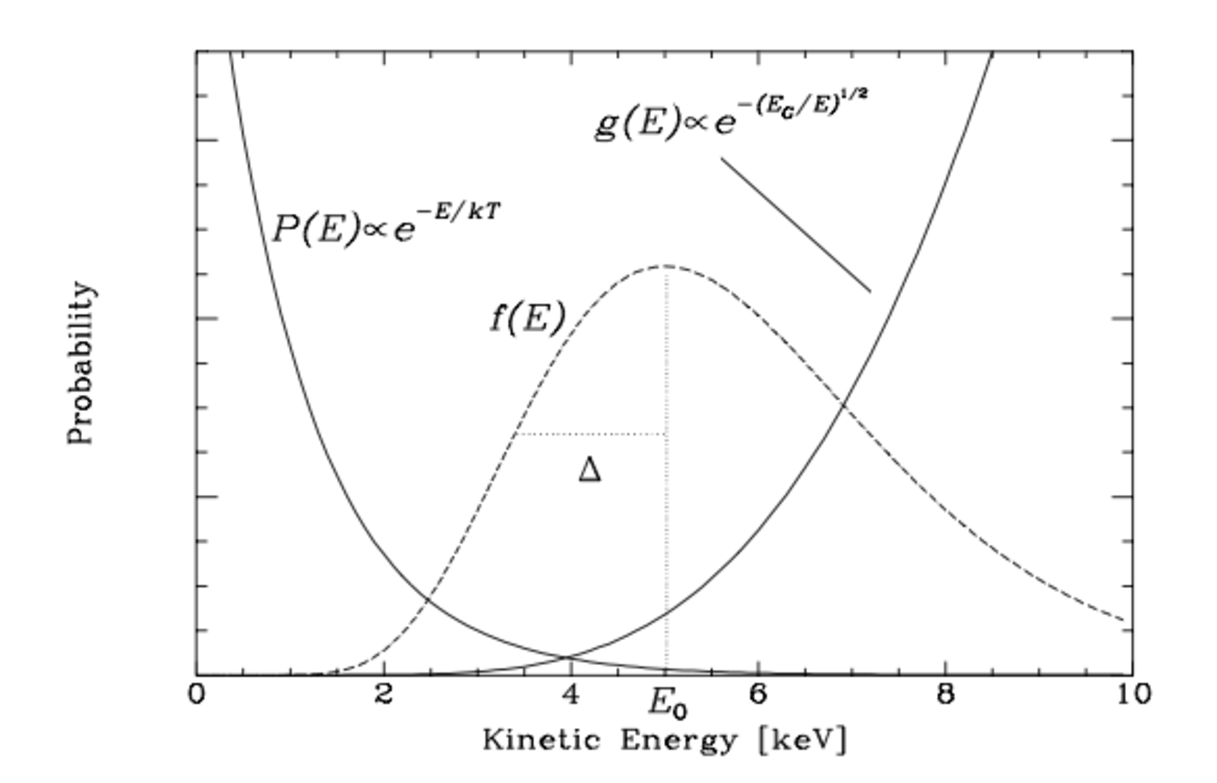
\includegraphics[width=.9\textwidth]{gamow_peak.pdf}
\end{center}
\end{figure}

This curve describes the range of kinetic energies over which nuclear reactions will take place.  The maximum is found by setting the derivative of Equation \ref{gamp} equal to zero, and thus

\begin{equation}
E_{o} = \left( \frac{kT}{2} \right)^{2/3} E_{G}^{1/3}.
\end{equation}

The greatest contribution to the nuclear reaction rate comes from a narrow energy band that depends on the temperature of the gas $T$, and the masses and charges of the reacting nuclei ($\mu$ and $Z_{1},Z_{2}$).

The energy generation rate, $\epsilon$ in Equation \ref{engen}, can then be found by doing some fancy math.  The important part is that it contains an exponential term that goes as 

\begin{equation}
\epsilon \propto \exp \left[ -3 \left( \frac{E_{G}}{4kT}\right)^{1/3} \right]
\end{equation}

Because of the Gamow energy in the exponential, there will be a strong preference for reactions between species with low atomic number, and thus small $E_{G}$; e.g., for similar abundances of deuterium and carbon in the center of star with kinetic energies typical of the Sun (1 keV), the p-p chain reactions would be heavily favored over the CNO cycle (see below for explanations of these reactions).

Also, the steep temperature dependence of nuclear reactions works as a "thermostat" in stars.  If $T$ increases inside a star, the rate of nuclear reactions will increase, $L$ will increase, the star will expand, which will cause $T$ to decrease, and the rate of nuclear reactions will decline accordingly.  Over the lifetime of the star, once the dominant nuclear fuel runs out, the rate of nuclear reactions will go down, the core will contract, and $T$ will rise until a new nuclear reaction involving nuclei of higher atomic number becomes favored\sidenote{This text is from Astrophysics in a Nutshell, pg. 57}.

\newthought{The following} are some relevant nucleosynthesis chains.  In each chain of the reactions, the following conservation laws must hold: conservation of electric charge, number of nucleons, and number of leptons\sidenote{The only way I can remember what constitutes a lepton is remembering that it means "light thing".  It includes electrons, positrons, neutrinos, and antineutrinos.}.

\begin{table}[h!]
\centering
\begin{tabular}{c c c}
\hline\hline
Reaction&$\gamma$&$\nu$\\
\hline
p-p & 1 & 4\\
CNO & 1 & 15\\
triple-$\alpha$ & 2 & 40\\
\hline\hline
\end{tabular}
\caption{Summary table for energy generation for various reactions, where $\epsilon \propto \rho^{\gamma} T^{\nu}$.}
\end{table}
 
 \begin{enumerate}
 \item \textbf{Proton-Proton Chain}: Chain of reactions which convert hydrogen to helium.
 
 \begin{equation}
 ^1_1H + \text{}^1_1H \rightarrow \text{}^2_1H + e^{+} + \nu_{e}
 \end{equation}
 \begin{equation}\label{ppstep2}
 ^2_1H + \text{}^1_1H \rightarrow \text{}^3_2He + \gamma
 \end{equation}
 \begin{equation}
 ^3_2He + \text{}^3_2He \rightarrow \text{}^4_2He + 2\text{}^1_1H
 \end{equation}
 
 The first step is the slowest because it involves the decay of a proton into a neutron (weak force).  There are two other p-p chain branches; the second p-p chain involves the interaction of the helium-3 produced in Equation \ref{ppstep2} with a helium-4 ($^7Be$ and $^7Li$ are intermediate products).  The third p-p chain involves the capture of an electron by the $^7Be$ nucleus created in the second p-p chain.  Most solar neutrinos come from the first p-p chain, but the highest energy ones come from the third p-p chain, despite this having a very low probability of occurrence.
 
 Important note: the total amount of energy released in forming the helium nucleus (binding energy) from four protons is $E_{b} = \Delta mc^2 = 26.731$ MeV.  That is, the combined mass of the four hydrogen atoms is greater than the mass of the resulting helium atom by $\Delta m = 26.731\text{MeV}/c^2$, or $0.7\%$ -- i.e. why hydrogen fusion has an efficiency factor of $.007$.
 
 \item \textbf{CNO Cycle}: This is another cycle for producing helium-4 from hydrogen.  The CNO cycle is more strongly temperature-dependent than the p-p chain, and is the dominant method of generating helium from hydrogen in massive stars ($\geq 1.2 M_{\odot}$) which have higher central temperatures (compared to low-mass stars, which predominantly use the p-p chain).  The CNO cycle uses carbon, nitrogen, and oxygen as catalysts and like the p-p chain has multiple branches\sidenote{I am too lazy to type them all out here, they are on pg. 311 in Carroll and Ostlie}.
 
Note: when hydrogen is converted into helium by either the p-p chain or the CNO cycle, the mean molecular weight $\mu$ of the gas increases, which (from the ideal gas law) means the central pressure will decrease.  That stellar core, no longer being in hydrostatic equilibrium, will begin to collapse.  This has the effect of raising the central temperature and density to compensate for the increase in $\mu$; once the temperature and density are high enough, helium nuclei can overcome their Coulomb repulsion and begin to fuse.\sidenote{This text is from Carroll and Ostlie pg. 312.  This page also has more information on the CNO cycle.}.
 
 \item \textbf{Triple-$\alpha$ Process}: This is the chain of reactions in which helium is converted into carbon-12.
 
 \begin{equation}
 ^4_2He + \text{}^4_2He \rightleftharpoons \text{}^8_4Be
 \end{equation}
 \begin{equation}
 ^8_4Be + \text{}^4_2He \rightarrow \text{}^{12}_6C + \gamma
 \end{equation}
 
 The beryllium nucleus produced by step one is unstable (even-numbered A) and will rapidly decay back into two heliums if it does not immediately interact with another helium nucleus.  The resonance of $^8_4Be + \text{}^4_2He$ with the energy of an excited state of carbon-12 greatly increases the probability of this second step occurring.
 \end{enumerate}

\section{Galaxies}
\subsection{Questions}
galaxies suck!!!!
\begin{enumerate}
\item Define two-body relaxation and estimate its time scale in (a) a globular cluster; (b)
      the Milky Way's disk. In which cases is two-body relaxation important?
\item Draw qualitatively the spectral energy distribution of the Milky Way, and describe
      how its morphology might appear to an external observer as a function of wavelength.
\item Describe at least three methods to probe the gravitational potential of galaxies,
      their assumptions, and their realm of applicability.
\end{enumerate}

\subsection{``The Galaxy''}

Let's describe the strucutre of the Milky Way here.  I'll begin with the thick vs thin disk
because that's interesting to me.

\newthought{In 1983, Gilmore and Reid} noted two separate structures within the disk of the
Milky Way: the thin disk ($\sim1$ kpc scale height) and the thick disk
($\sim5$ kpc scale height).  The distinction (apart from the obvious difference in dynamics)
is that the thick disk consists of an older population of stars while the thin disk consists
of a younger population of stars.
The stars in the thick disk are believed to be have been formed in a thinner disk and then
excited to larger scale heights through encounters with satellite galaxies or mergers.
The thin disk is believed to have been formed by gas
accretion at later times during the formation of the galaxy.

I believe we had a colloquium earlier this year (or last year) that used SDSS data to show
that there is no thin disk/thick disk distinction but rather a continuous distribution
where the scale height of a stellar population scales with its age.


\section{The Interstellar Medium}

I added sections based on the list of important topics Allison gave us 
before the final. 

\subsection{Questions}
\begin{enumerate}
\item \textbf{Draw the cooling function for gas of solar metallicity, and describe the cooling
      mechanisms in each part of the curve. Explain the relevance of this function to multi-
      phase ISM models.}
      
      Figure \ref{f:cool1} shows the cooling function $\Lambda$ as a function of $T$ (note that in class, Nick showed us a cooling curve of $T$ vs. $n$). At $T < 10^3$ K, the cooling is from molecular line emission. The plateau from $\sim10^3$ to $\sim10^4$ K is due to collisionally excited lines of neutral and low-ionization metals. There is a peak around $\sim10^4-10^5$ K, which is due to recombination of hydrogen (i.e. hydrogen recombines and then downward transitions emit low-energy photons such as H$\alpha$ that find the HII region optically thin). There is a quadruple peak at $T \approx 10^5,~2\times 10^5,~5\times 10^5,~10^6$ K from far-UV and X-ray emission lines from highly ionized species of C,O,Ne,Fe, respectively. At $T > 10^7$ K, most of the cooling is from Bremsstrahlung.
      
      \begin{figure}[ht]
      \begin{center}
      \includegraphics[width=\textwidth]{ism_Q1_cool.jpg}
      \end{center}
      \caption{Cooling curve from Astrophysics in a Nutshell. \label{f:cool1}}
	  \end{figure}
	
	  Figure \ref{f:cool2} is a more detailed version from Nick's notes, and it goes to higher temperature.
	
	  \begin{figure}[ht]
      \begin{center}
      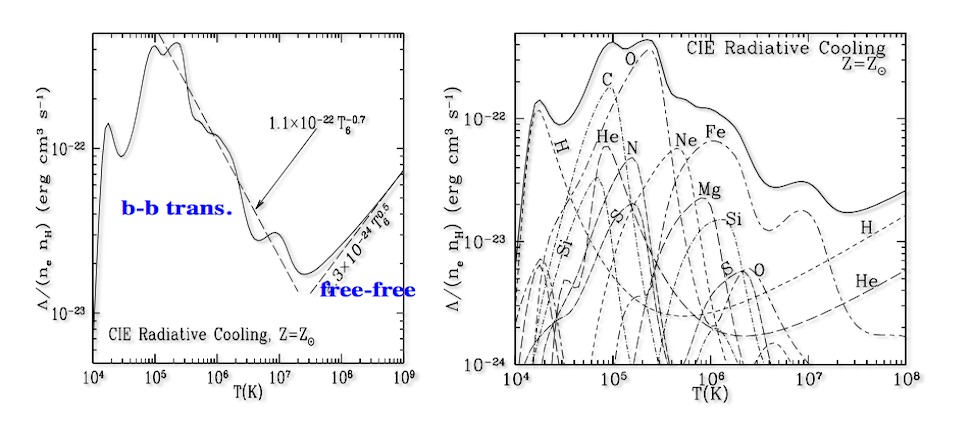
\includegraphics[width=\textwidth]{ism_Q1_cool_b.jpg}
      \end{center}
      \caption{Cooling curve from Nick's notes with more details on relevant elements. \label{f:cool2}}
      \end{figure}

      \newthought{So how does} the cooling function relate to the multi-phase\sidenote{
            Here we take ``phase'' to mean a particular temperature, density, and ionization
            state of the ISM.  I (Michael) believe we use the word ``phase'' to indicate that not
            all combinations of temperature and density are possible -- there are distinct
            regions of phase-space that define the characteristics of the ISM.
      } nature of the ISM?
      To understand this, let's suppose the ISM is composed of two or more distinct phases.
      The boundary between these two phases (assuming the boundary between them is at least
      quasi-stable) must satisfy pressure equilibrium such that $n_1T_1=n_2T_2$.  Additionally,
      each phase must have cooling balanced by heating, and be stable to temperature
      perturbations\sidenote{
            This means that if the temperature is increased, cooling dominates heating, and if
            the temperature is decreased, heating dominates cooling.
      }.
      Therefore, areas where the cooling function decreases as a function of temperature
      (cooling increases as temperature decreases) are likely to be unstable.  However, for a more
      detailed treatment of cooling and heating, one must consider the balance $n^2\Lambda(T) = n\Gamma(T)$
      for an arbitrary cooling function $\Lambda$ and heating function $\Gamma$.
      
\item \textbf{Draw a typical spectrum of an HII region, including both lines and continuum, and
      explain the major processes that give rise to each feature.}
      
      Figure \ref{f:HIIspec} shows a spectrum of an HII region with the continuum removed. The spectrum is similar to that of a planetary nebula (a ball of mostly-hydrogen gas ionized by the newly formed white dwarf instead of a young star). The hydrogen features are from transitions to the $n=2$ state (no Lyman features are pictured here, but ${\rm Ly}\alpha$ should be there) of 
      
      \begin{figure}[ht]
      \begin{center}
      \includegraphics[width=\textwidth]{ism_Q2_HII_spec.jpg}
      \end{center}
      \caption{Spectrum of an HII region with the continuum removed. \label{f:HIIspec}}
	\end{figure}
	
	 The spectrum is similar to that of a planetary nebula (a ball of mostly-hydrogen gas ionized by the newly formed white dwarf instead of a young star). The Hydrogen features are from transitions to the $n=2$ state (no Lyman features are pictured here, but ${\rm Ly}\alpha$ should be there). 
	 
	 The other prominent features are from singly- and doubly-ionized Oxygen bound-bound transitions. These ions are important coolants in HII regions and act as thermostats for the gas. Free electrons zooming around will collisionally excite the Oxygen ions to an excited state, which will then decay and radiate line emission. The gas is optically thin to these lines, so they are very prominent in the spectra. 
	 
	 \emph{An Explanation of Oxygen Cooling in HII Regions--} The Oxygen ions help maintain the temperature of the HII region at a steady 10,000 K. This is because they are collisionally excited. If the gas is hotter than 10,000 K, the increased velocity of the free electrons increases the number of collisions, converting the excess kinetic energy into line emission which escapes the gas. If the gas is cooler than 10,000 K, the lower velocity reduces the number of collisions, and hence the amount of cooling. This allows the gas opportunity to gain energy and increase its temperature back up to 10,000 K.\emph{end side note}
	 
	 The continuum from the HII region is from the star, and from recombination. I wish I had figures of either of these but I couldn't find any. The star's blackbody is modified as the Hydrogen absorbs any wavelength shortward of the Lyman limit of 912\AA. Remember that wavelengths closer to that number are absorbed preferentially, so photons of much higher energy are not attenuated as much. This manifests as a sharp drop of stellar flux at the Lyman limit, and then a slight rise toward shorter wavelengths. I actually found a figure of this situation but I forgot which book it was in and couldn't find it again... Basically this is what makes the stellar spectrum 'harder' toward the edge of the HII region: all the flux right at the Lyman limit has been absorbed, so the far UV flux is higher than the near UV flux. The longer wavelengths of the star's spectrum is mostly left untouched.
	 
	 As Hydrogen can be ionized by many possible wavelengths, the free electrons that result can have a continuum of energies. This also means that when one of these free electrons recombines with Hydrogen, the first photon it releases can have a continuum of energies. This is called the "recombination continuum". Unfortunately I have no idea what it looks like in a spectrum...
	 
	 
\item \textbf{Explain quantitatively what determines the temperature of dust grains and their
      thermal emission spectrum. Give examples of astrophysical environments with different
      dust temperatures.}
\end{enumerate}

	First, let's remember what dust is. Dust grains are macroscopic particles of mostly ices and metals in solid form. With radii of $r \sim 1 nm - 0.1 \mu m$, they are around the same size of what we'd consider 'smoke'. Because they are macroscopic, their emission is based on their \textbf{temperature}. A gas's temperature is determined by interactions with a radiation field, but also by collisions between the particles. Dust temperature, however, is only determined by equilibrium with the radiation field. Hence, \emph{mixed gas and dust can have different temperatures}. 
	
	Dust absorbs preferentially bluer light, depending on the grain's size. In class we had a homework problem where the fraction of light absorbed was defined as:
	
	\begin{equation}
	Q_{abs} = (\frac{2\pi a}{\lambda})^{n}
	\end{equation}
	
	where $a$ is the radius of the dust grain, and $n$ is a positive number. If the grain is very large, or the photon wavelength is very small, all light will be absorbed. This quantity comes into play in the definition of the dust absorption coefficient:
	
	\begin{equation}
	\kappa_{\lambda} = \pi a^{2} Q_{abs} n_{dust}
	\end{equation}
	
	For the typical sizes of dust grains, in a region where the incident flux is dominated by UV light, one can approximate as all the incident flux being absorbed by the dust. 
	
	This coefficient, in a detailed treatment, also affects the emission of the dust grain, where:
	
	\begin{equation}
	j_{\lambda} = \kappa_{\lambda} B_{lambda}(T_{dust})
	\end{equation}
	
	This describes the emission as a blackbody at equilibrium dust temperature $T_{dust}$ modified by the opacity. 
	
	In the approximation that the dust emits completely like a blackbody, $n = 1$ and one finds the temperature of the dust as function of distance from a nearby star:
	
	\begin{equation}
	T_{dust}(r) = \sqrt{\frac{R_{*}}{2r}}T_{*}
	\end{equation}	
	
	

\subsection{Useful Numbers and Relations}
$2\times10^{21}$ H cm$^{-2}$ for $1$ mag of visual extinction\newline
\newline
$30$ mag of visible extinction towards Galactic Center\newline
\newline
$13.6$ eV=$912$ \AA=shock with v$>50$ km/s\newline
\newline
$\frac{E}{eV}=\frac{T}{10,000 K}$\newline
\newline
H photoionization cross section $\sigma_{\nu}=6\times10^{-18}(\nu/\nu_0)^{-3}
cm^2$\newline
\newline
mean free path = $1/(n\sigma)\sim 1.6\times10^{17}/n_H$ cm\newline
\newline
$v_{sound}=\sqrt{\frac{\gamma kT}{m}}$\newline
\newline
For atomic H and $\gamma=5/3$,\newline
\newline
$\frac{v_{sound}}{km/s}=\sqrt{\frac{T}{100 K}}$

\subsection{Basic Things about ISM Phases}

The ISM phases are characterized by the state of hydrogen gas.

H$_2$ (molecular): $n \sim 200-10^6~{\rm cm}^{-3}$, $T \sim 10-500~{\rm K}$

Exists in molecular clouds and dark clouds, as well as protostellar cores.  
Molecular and dark clouds (lower end of the temperature and density range) are 
detected based extinction of background stars.  Giant molecular clouds 
have temperatures of $50-100$ K and and are heated by newly formed massive 
stars.  These are also seen in extinction, and in line emission in the far-IR 
and radio.  The molecular H itself is very difficult to detect 
spectroscopically, but other molecules in the clouds such as CO can be 
detected.  Giant molecular clouds have masses of 
$10^3-10^6\ M_{\odot}$.  The hottest and densist H$_2$ is found in protostellar 
cores, which are collapsed regions of GMCs.  

HI (atomic): $n \sim 1-100~{\rm cm}^{-3}$, $T \sim 100-3000~{\rm K}$

Atomic H is found in diffuse clouds.  These clouds are semitransparent, with 
visual extinction of $\sim1$ mag.  The are observed using $21$ cm emission 
(warmer clouds) and absorption (cooler clouds).  In the centers of the clouds, 
molecules such as CO and OH can form and be shielded from starlight.  These 
clouds are also visible in the infrared from their blackbody radiation.  
 
HII (ionized): $n \sim 0.1-10^3~{\rm cm}^{-3}$, $T \sim 10^4-10^6~{\rm K}$

Ionized H is found in emission nebulae (planetary nebulae, supernova remnants, 
and HII regions).  Observationally, ionized H can be observed using H 
recombination lines (such as H$\alpha$) and other atomic recombination lines 
such as [OIII].  Bremsstrahlung emission is also seen in these regions.  
Supernova remnants and planetary nebulae have well defined shell-like shapes 
and are associated with individual stars.  HII regions appear fuzzy and 
are associated with sites of multiple star formation and molecular clouds.  
Planetary nebulae can also be distinguished from HII regions from line ratios.  
The star at the center of a planetary nebula is the core of an evolved star, 
and can be $>10^5$ K.  This produces much higher energy photons than those 
in HII regions, so ratios of [OIII] to H$\alpha$ are higher in planetary 
nebulae, and even He recombination lines are weakly visible.  

Ionized H can also be found in galactic coronal gas in the halo.  This gas 
is most likely heated $10^5-10^6$ K gas is most likely heated by shocks from 
multiple supernovae.  It can be detected from X-ray emission and UV absorption.
 
 Transitions between phases:
 
 Ionization of neutral hydrogen requires $13.6~{\rm eV}$, or photons with wavelength $\lambda < 912 \AA$, OR shocks that are faster than $50~{\rm km/s}$. In HII regions around hot (O,B) stars, the hydrogen is photoionized by the UV radiation from the star, and there are very sharp transitions between the HII, HI, and H$_2$ regions around the star.

\subsection{Heating and Cooling}
The example of heating and cooling we did in class was for an HII region.  
According to the slides, the same derivation can be followed for other 
phases of the ISM, just with different transitions.  

In an HII region, gas is heated when a photon with energy $>13.6$ eV ionizes 
a neutral H atom.  This gives the free electron extra kinetic energy, which 
it transfers to the gas.  The rate of heating is just the rate at which 
energy is transferred into the gas by this method.  So the heating rate 
$\Gamma$ is the photo-ionization rate times the extra energy per 
photo-ionization.
\begin{equation}
\Gamma=R_{ph}\times\bar{E}
\end{equation}
Since the HII region is fully ionized, photo-ionizations can only take 
place at the rate of recombinations (this is basically saying ionization 
equilibrium is maintained.  So the rate of photo-ionizations equals the rate 
of recombinations:
\begin{equation}
R_{ph}=n_en_p\alpha_B
\end{equation}
where $\alpha_B$ is the recombination rate coefficient into levels higher than 
n$=1$.  Things get confusing here with these $\alpha$s.  There's a total $\alpha$ 
for all recombinations, an $\alpha_A$ for recombinations to n$=1$, and 
$\alpha_B$.  Kwok says $\alpha_B$ should be used here.  The lecture slides 
say it should be $\alpha_A$, but later in the derivation, it looks like this 
magically turns into $\alpha_B$.  I'm assuming the $\alpha_A$ in the lecture 
slides is a typo, and we should be using $\alpha_B$.  This makes sense 
physically, because we want to know the rate of recombinations that allow 
a photon from the central star to ionize an atom.  If a recombination happens 
directly to n$=1$, then a photon will be emitted with enough energy to 
ionize a new atom.  So the photon from the star that is trying to heat the gas 
will still have nothing new to ionize.  If the recombination happens to a 
higher energy level, and the electron cascades down to n$=1$, several photons 
will be emitted, but none will be able to ionize anything.  So the net result 
is there is now a new neutral atom that can be ionized by the star.  If this 
is all still too confusing, we can probably get away with just saying $\alpha$ 
and ignoring this whole A or B business. 

Meanwhile, back at the ranch, we need the average energy given to an electron 
in a photo-ionization.  The kinetic energy given to the electron by a photon 
of frequency $\nu$ is just $h(\nu-\nu_0)$ where $\nu_0$ is the frequency 
required to ionize H.  The total energy added by this frequency is the 
energy from one photon times the number of photons at that frequency, given 
by the intensity of the radiation field divided by the photon energy.  
Integrating over all frequencies above the ionization frequency, and dividing 
by the total number of photons gives the average kinetic energy given.   
\begin{equation}
\bar{E}=\frac{\int_{\nu_0}^\infty{h(\nu-\nu_0)\frac{J_{\nu}}{h\nu}a_{\nu}\,d\nu}}{\int_{\nu_0}^\infty{\frac{J_{\nu}}{h\nu}a_{\nu}\,d\nu}}
\end{equation}
$a_{\nu}$ is the photo-ionization cross section.  Defining $T_i$ such that 
\begin{equation}
\bar{E}=\frac{3}{2}kT_i
\end{equation}
results in 
\begin{equation}
\Gamma=n_en_p\alpha_B\frac{3}{2}kT_i
\end{equation}
For $J_{\nu}$ from a central star of temperature $T_*$ and 
$a_{\nu}\propto\left(\frac{\nu}{\nu_0}\right)^3$, $T_i\sim T_*$.

One way an HII region can cool is through recombination to energy levels 
above n$=1$, followed by a cascade to n$=1$.  Assuming all the H in the region 
is in the ground state, the emitted photons will escape the HII region, and 
kinetic energy will have been removed.  The rate at which this happens is 
\begin{equation}
\Lambda=n_en_pkT\beta
\end{equation}
where 
\begin{equation}
\beta=\alpha_B\int_0^\infty{\frac{1}{2}mv^2\frac{\sigma_vv}{kT_e}f(v)\,dv}
\end{equation}
The integral includes the kinetic energy lost by the electron, $\sigma v$, 
which has appeared in rate equations before that we've had (I don't remember 
why), and the distribution of velocities.  Re-writing the cooling rate to 
look more like the heating rate,
\begin{equation}
\Lambda=n_en_p\alpha_B\bar{E}
\end{equation}
For $\sigma_v\propto v^{-2}$, $\bar{E}\sim0.4\times\frac{3}{2}kT_e$.
So
\begin{equation}
\Lambda=n_en_p\alpha_B0.4\times\frac{3}{2}kT_e
\end{equation}
Setting heating equal to cooling to find the gas temperature ($T_e$) gives
$T_e\sim1.7T_*$.  The O and B stars at the center of HII regions are 40,000-
50,000 K, but the gas in the region is only around 10,000 K.  So H 
recombination is not enough to cool the gas to the observed temperatures.  
Free-free emission can cool the gas to about $T_*$, but this is still not 
enough.  The most important coolent of the gas turns out to be line transitions 
in metal ions.  Collisional excitations remove kinetic energy from the gas, 
followed by photon emission.  The gas is optically thin to these photons, 
so the photons escape and carry the energy away.

By the way, there's a simplified 
version of all this in chapter 5 of Astrophysics in a Nutshell.  The reason I followed Nick's 
slides is he actually plugs in numbers to show that H cooling is not enough to cool an HII region 
to the observed temperatures.  Nick doesn't plug in any numbers from this point on though, 
so I'm switching to Astrophysics in a Nutshell for metal cooling.

The basic picture of metal cooling starts with free electrons colliding with ionized species of 
C, N, O, S, Si, Fe, and other elements.  The electrons have kinetic energies that match the 
excited states of these atoms, so the atoms are excited and kinetic energy is removed from the 
gas.  If the atoms can decay by emitting a photon before another collision puts that kinetic 
energy back into the gas through collisional deexcitation, the photon can escape the HII region 
and carry away the energy, cooling the region.  The photon can escape because these metals have a 
low abundance, so it is unlikely to be absorbed by another atom.  Also, if forbidden transitions 
are involved, re-absorption is even less likely.  

Consider an atom with energy levels level $1$ and level $2$.  The cooling rate for this 
transition is given by the radiative transition rate times the energy.
\begin{equation}\label{eq:cooling}
\Lambda=n_2A_{21}h\nu
\end{equation}
where $A_{21}$ is the Einstein A coefficient that determines the rate.  The collisional excitation 
rate from level $1$ to level $2$ is given by 
\begin{equation}
R_{12,coll}=n_en_1q_{12}=n_e(n-n_2)q_{12}
\end{equation}
where $q_{12}$ is a coefficient for that rate that includes temperature and cross section 
effects.  The collisional deexcitation rate is 
\begin{equation}
R_{21,coll}=n_en_2q_{21}
\end{equation}
The radiative decay rate is 
\begin{equation}
R_{21,rad}=n_2A_{21}
\end{equation}
Stimulated emission can be ignored in HII regions (although it is important for masers).  
Balancing excitations with deexcitations and solving for $n_2$ gives:
\begin{equation}
n_2=\frac{n_enq{12}}{n_e(q_{21}+q_{12})+A_{21}}
\end{equation}
Plugging this into Equation \ref{eq:cooling} gives
\begin{equation}
\Lambda=\frac{n_enq_{12}A_{21}h\nu}{n_e(q_{21}+q_{12})+A_{21}}=\frac{n_enq_{12}h\nu}{(1+q_{12}/q_{21})n_eq_{21}/A_{21}+1}
\end{equation}
Defining $n_{crit}\equiv A_{21}/q{21}$ results in 
\begin{equation}\label{eq:cooling2}
\Lambda=\frac{n_enq_{12}h\nu}{(1+q_{12}/q{21})n_e/n_{crit}+1}
\end{equation}
The ratio of q's in the denominator is given by 
\begin{equation}
\frac{q_{12}}{q_{21}}=\frac{g_2}{g_1}e^{-h\nu/kT}
\end{equation}
For any temperature, this ratio is of order 1 or less.  Therefore, if $n_e<<n_{crit}$, the first 
term in the denominator of Equation \ref{eq:cooling2} can be ignored, and 
$\Lambda\propto n_en\sim n_e^2$.  For $n_e>>n_{crit}$, the first term dominates and 
$\Lambda\propto n\sim n_e$.  H recombination and bremsstrahlung cooling always go as $n_e^2$, 
so for high densities, these processes are more efficient than metal cooling.  

An important cooling line for HII regions is the [O III] forbidden doublet at 4959 and 5007 \AA.  
At densities lower than the critical density for this line of $\sim10^6$ cm$^3$, the long lifetime 
of the excited state (it's a forbidden line) is still shorter than the time between collisions, 
so the atom deexcites by emitting a photon.  

Metal lines keep the temperature of HII regions at around $10^4$ K, independent of the temperature 
of the central star.  If the central star is hot and produces lots of high energy photons, this 
will heat the gas more efficiently because freed electrons will have more energy.  Because these 
electrons are moving faster, however, the collision rate between the electrons and metal ions 
will increase, also making cooling more efficient.  These effects balance to keep the 
HII temperature at around $10,000$ K.  

Also useful to know for heating and cooling- in intracluster gas between galaxies, temperatures 
are hot enough that everything is ionized, and densities are low enough that recombinations 
are rare.  In this situation, bremsstrahlung is the most efficient coolant.  Bremsstrahlung 
cooling is not very effective, however, particularly at these densities, which is why this 
gas stays so hot (and why the cooling curve drops above $10^6$ K, see will-ask).

The basic take-home here is things are heated when something comes in and adds kinetic energy.  
This can be a photon that can ionize something, giving an electron kinetic energy, cosmic rays 
which can collide with particles and give them kinetic energy, or shocks which give kinetic 
energy to large amounts of gas all at once.  Cooling happens through recombination or collisional 
excitation and radiative deexcitation if the photons can escape.  If everything is ionized, 
then bremsstrahlung cools the gas.  This can be applied to any region, for example a molecular 
cloud is cooled by CO (I think) the same way an HII region is cooled by [O III].


\subsection{Line Emission}
Forbidden Lines:\newline
These are lines that violate the transitions rules:
\begin{displaymath}
\Delta L=\pm1\ or\ 0
\end{displaymath}
\begin{displaymath}
\Delta S=0
\end{displaymath}
\begin{displaymath}
\Delta J=0,\ \pm1\ except\ 0\ to\ 0
\end{displaymath}
These transitions can occur through electric quadropole or magnetic dipole transitions, but these 
have much longer lifetimes (how much longer?) than allowed transitions.  Because of this, in the 
lab, atoms will collisionally deexcite before radiatively decaying by a forbidden transition.  
In the ISM, however, densities are low enough (below the critical density, see heating and 
cooling), that these forbidden transitions can happen.  Forbidden lines make important coolents 
and are observationally very strong because the upward transitions are forbidden as well, so once 
a forbidden photon is emitted, it is unlikely to be reabsorbed.  Atoms can be excited to forbidden 
levels by collisions, so getting the atoms excited in the first place is not a problem.  Forbidden 
lines in nebulae tend to be as strong as H recombination lines because even though metals are 
much less abundant than H, collisional excitation is a much faster process than H recombination 
in nebulae.  

Determning Density and Temperature:
Density of a nebula can be determined using the intensity ratio of two forbidden lines with 
similar energy but different critical densities (different A coefficients).  For example, 
this can be done with the [O II] doublet at $3726$ and $3729$ \AA.  This corresponds to transitions 
from the $^2D_{3/2}$ and $^2D_{5/2}$ states.  Since these lines are optically thin, the intensity 
observed will just be proportional to the emission.  Call $^2D_{3/2}$ level $3$ and $^2D_{5/2}$ 
level $2$, with both transitions going to level $1$.  Assuming the energy emitted in each 
transition is $\sim$the same and there are no transitions between levels $2$ and $3$, then
\begin{equation}\label{eq:Irat}
\frac{I_{31}}{I_{21}}=\frac{n_3A_{31}}{n_2A_{21}}
\end{equation}
Using detailed balance for the $2\rightarrow1$ transition:
\begin{equation}
n_2(A_{21}+n_eC_{21})=n_1n_eC_{12}
\end{equation}
Solving for $\frac{n_2}{n_1}$ gives
\begin{equation}
\frac{n_2}{n_1}=\frac{n_eC_{12}}{A_{21}}\left(\frac{1}{1+\frac{n_eC_{21}}{A_{21}}}\right)
\end{equation}
A similar equation can be derived for $\frac{n_3}{n_1}$.  Using these equations to determine 
the ratio of $n_3$ to $n_2$ and plugging into Equation \ref{eq:Irat} gives
\begin{equation}
\frac{I_{31}}{I_{21}}=\frac{C_{13}}{C_{12}}\frac{1+\frac{n_eC_{21}}{A_21}}{1+\frac{n_eC_{31}}{A_31}}
\end{equation}
The A's in this equation are constants that can be looked up.  The ratio of the C's is given by 
a Boltzmann distribution, which depends on the statistical weights of each level (constants) and 
exponentially on the energy of the transitions and the temperature.  The energies of the two 
transitions are $\sim$the same and the temperature is just whatever the gas temperature is, so 
the exponentials cancel out.  So, the only free parameter 
is the density, and by measuring the ratio of the line strengths, the density can be determined.  
Another doublet that this can be done with is [S II] (6716 and 6731 \AA).

Temperature can be determined in a similar way using three transitions, including a doublet.  
An example is the [O III] lines at 4363, 4959, and 5007 \AA.  These correspond to the transitions
$^1S_0\rightarrow ^1D_2$, $^1D_2\rightarrow ^3P_1$, and $^1D_2\rightarrow ^3P_2$.  Call the S 
level $3$, D level $2$, and both P levels level $1$.  Assume the gas is low density, so that every 
collisional excitation results in a radiative deexcitation, and that levels $2$ and $3$ can only 
be populated by collisional excitation from level $1$.  With these assumptions, 
\begin{equation}\label{eq:I3rat}
\frac{I(4363)}{I(5007)+I(4969)}=\frac{n_3E_{32}A_{32}}{n_2E_{21}A_{21}}
\end{equation}
The denominator in Equation \ref{eq:I3rat} is because we assumed any atoms in level $2$ must 
radiatively decay to level $1$, and both of these doublet transitions have $\sim$the same energy.  
Using detailed balance in levels $2$ and $3$, assuming only collisional excitation and radiative 
deexcitation are important:
\begin{equation}
n_2A_{21}=n_1n_eC_{12}
n_3(A_{31}+A_{32})=n_1n_eC_{13}
\end{equation}
This is basically a statement that every collisional excitation must be followed by a 
radiative deexcitation.  The reason the level $2$ equation does not include transition into 
level $2$ from level $3$ is because we're not trying to balance an equilibrium population in level 
$2$.  In equilibrium, everything is in level $1$, because anything that gets excited decays right 
away.  All we're doing is saying a collision happens that can send the atom into level $2$ or 
level $3$.  The first balance equation describes the first case, and the seond describes the 
second case.  Temperature comes into play because it determines the speed of the colliding 
electrons and atoms.  If it's really hot, and there are only ever collions up to level $3$, the 
ensuing decays will produce a certain line ratio.  If it's cold, and only collisions to level $2$ 
can happen, their will be no transitions from $3$ to $1$, so the line ratio will be $0$.  The 
temperature determines the ratio of collisions into $2$ to collisions into $3$, and the line 
ratio directly follows from this.  

Going through the rest of the math, solving for the ratio of $n_3$ to $n_2$ and plugging into 
Equation \ref{eq:I3rat} gives
\begin{equation}\label{eq:Iratfinal}
\frac{I(4363)}{I(5007)+I(4969)}=\frac{C_13}{C_12}\frac{\nu_{32}}{\nu{21}}\frac{A_{32}}{A_{31}+A_{32}}\propto\frac{C_13}{C_12}
\end{equation}
\begin{equation}
\frac{I(4363)}{I(5007)+I(4969)}\propto\frac{\Omega_{13}}{\Omega_12}e^{-E_{32}/kT}
\end{equation}
The $\Omega$'s are collisional strength, which can be looked up, so the only free parameter is 
temperature.  Getting from C to $\Omega$ requires a bunch of equations in Kwok that we don't need 
to waste our time on.  If we actually have to go through all this math on the qual, I say 
we stop at Equation \ref{eq:Iratfinal} and say the C's depend on an exponential term involving 
temperature, so knowing the line ratios gives the temperature.  This proceedure can also be 
done for higher densities, but then the detailed balance equations include more collisional terms 
and are more complicated.  

\subsection{HII regions}
HII regions are created by young O and B stars, which produce large numbers of UV photons capable 
of ionizing the H clouds these stars are born in.  To ionize significant amounts of H, these 
stars need temperature $>25,000$ K.  The initial size of an HII region is determined by 
balancing the flux of ionizing photons from the star with the rate of recombinations.  As the 
HII region is heated, the pressure inside becomes much greater than the pressure of the 
surrounding neutral cloud, and the region dynamically expands.  This lowers the density in the 
region, allowing more ionizing photons to get out and ionize additional material.  This continues 
until pressure and ionization equilibrium are reached with the surrounding cloud.  In reality, 
however, the O and B stars powering HII regions will supernova before this final state is 
achieved.  Note- I'll be using the word expansion a lot in this section, so I'll try to be as 
specific as I can what I mean.  Ionization expansion means new material is being ionized, so 
the size of the HII region ``expands'', but the gas itself is staying where it is.  Dynamical 
expansion means the already ionized gas is out of pressure equilibrium, so the gas itself moves 
outwards and the regions physically expands into the surrounding cloud.  

The initial size of an HII region is defined by the \emph{Stromgren sphere}, which assumes 
a uniform, non-expanding medium of neutral H surrounding a star that turns on at $t=0$.  The 
star's output rate of ionizing photons is $N_u$ and the density of the surrounding medium is 
$n_0$.  Initially, all of the ionizing photons from the star go into ionizing new material.  
In a time $dt$, the star puts out $N_udt$ ionizing photons.  These photons ionize a shell of 
thickness $dR$ which contains $N_udt$ neutral H atoms.  So the ionization expansion is governed 
by the equation
\begin{equation}\label{eq:earlyHII}
N_u=n_04\pi R^2\frac{dR}{dt}
\end{equation}
The solution is 
\begin{equation}
R(t)=\left(\frac{3N_u}{4\pi n_0}t\right)^{1/3}
\end{equation}
After a short time (the actual time can probably be estimated from the density and the 
recombination coefficient), recombination becomes important, and the photons from the star are 
must keep material ionized in addition to ionizing new material.  The rate of recombination 
rate per unit volume is given by 
\begin{equation}
N_{rec}=\alpha n_en_p=\alpha n_0^2
\end{equation}
Multiplying this by the volume of the HII region and including it on the right hand side of 
Equation \ref{eq:earlyHII} gives
\begin{equation}
N_u=4\pi n_0R^2\frac{dR}{dt}+\alpha n_0^2\frac{4\pi}{3}R^3
\end{equation}
which has the solution
\begin{equation}
R(t)=R_S\left(1-e^{-t/t_S}\right)^{1/3}
\end{equation}
with $t_S=\frac{1}{\alpha n_0}$ and the \emph{Stromgren radius} defined as 
\begin{equation}
R_S\equiv\left(\frac{3N_u}{4\pi \alpha n_0^2}\right)^{1/3}
\end{equation}
For a typical HII region with $T\sim10^4$ K, $\alpha=2.6\times10^{-13}$ cm$^3$s$^{-1}$.  
Assuming $n_0\sim30$ cm$^{-3}$ and an O$5$ star with $N_u=4\times10^{46}$ s$^{-1}$, 
$R_S\sim4\times10^{19}$ cm $\sim12$ pc.  The timescale to create this sphere is $t_S\sim4000$ yr.
The transition from the HII region to the surrounding medium will be very sharp, of order 
the mean free path of an ionizing photon (why?), $\lambda_i=1/(n_0\sigma_i)$, where 
$\sigma_i=6\times10^{-18} $cm$^2$.

This all assumes a static sphere, which is not realistic.  The temperature inside the HII region 
will be $\sim10^4$ K, compared to $\sim100$ K in the surrounding gas.  Also, the HII region has 
twice as many particles once it is ionized, so the pressure in the region is $\sim200$ times the 
pressure of the neutral gas.  As the HII region expands, and shock front and ionization front 
develop.  Let $\Phi_i$ be the ionizing flux from the star at the ionization front, $P_1$ and 
$\rho_1$ be the pressure and density of neutral gas, and $u_1$ be the velocity of the neutral 
gas relative to the ionization front.  Let $\rho_2$, $P_2$, and $u_2$ be the density, pressure, 
and relative velocity of the ionized material inside the HII region.  Across the ionization front, 
the usual mass and momentum conservations equations hold:
\begin{equation}
\rho_1u_1=\rho_2u_2
\end{equation}
\begin{equation}
P_1+\rho_1u_1^2=P_2+\rho_2u_2^2
\end{equation}
Also, any mass that crosses the ionization front must become ionized, so the flux of particles 
across the front must equal the flux of ionizing photons:
\begin{equation}
\rho_1u_1=m_i\Phi_i
\end{equation}
where $m_i$ is the mean particle mass of the ionized gas.  Defining the sound speeds in the 
neutral and ionized material as $a_1=(P_1/\rho_1)^{1/2}$ and $a_2=(P_1/\rho_1)^{1/2}$, the 
mass and momentum equations can be solved for $\rho_2/\rho_1$ in terms of these sound speeds 
and $u_1$.  
\begin{equation}\label{eq:ratio}
\frac{\rho_2}{\rho_1}=\frac{1}{2a_2^2}(a_1^2+u_1^2\pm\sqrt{f(u_1)})
\end{equation}
where $f(u_1)=(a_1^2+u_1^2)^2-4a_2^2u_1^2=(u_1^2-u_R^2)(u_1^2-u_D^2)$, with 
\begin{equation}
u_R\equiv a_2+\sqrt{a_2^2-a_1^2}
\end{equation}
\begin{equation}
u_D\equiv a_2-\sqrt{a_2^2-a_1^2}
\end{equation}
The density ratio must be real, either $u_1\geq u_R\geq u_D$ or $u_1\leq u_D\leq u_R$.  The 
first case (rapidly moving ionization front) is called an R-type front.  The second is a 
slower D-type front.  In an R-type front, $u_1>u_R>a_2>a_1$, so the shock into the neutral medium 
is supersonic.  In a D-type front, $u_1<u_D<a_1<a_2$, so the shock is subsonic.  

\begin{figure}[!h]
\begin{center}
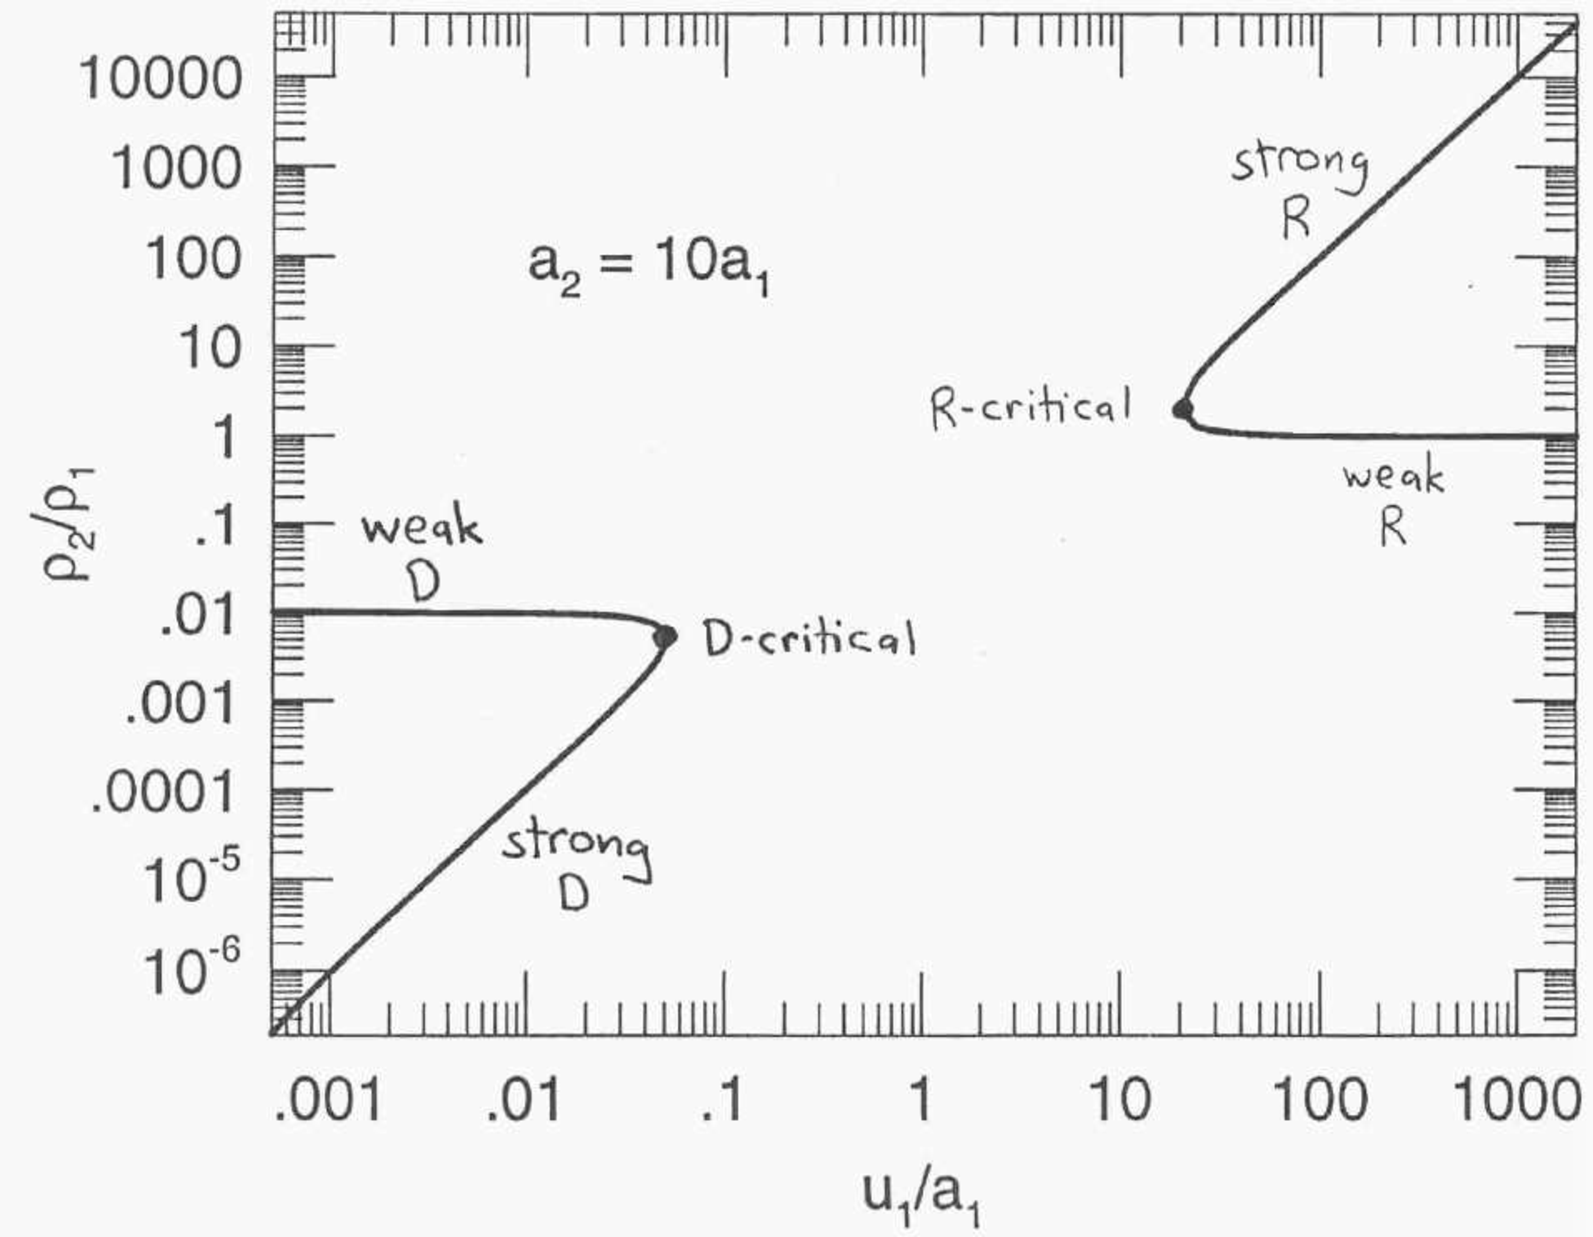
\includegraphics[width=\textwidth]{shock_plot.pdf}
\end{center}
\caption{Density vs. Velocity in an expanding HII region \label{fig:shock}}
\end{figure}

For every ionization front velocity $u_1$, there are two possible density ratios because of the 
plus-minus sign in Eqaution \ref{eq:ratio} (see Figure \ref{fig:shock}.  The larger ratio is a 
\emph{strong front}, and the smaller ratio is a \emph{weak front}.  Strong R-type fronts are 
unstable, but weak R fronts and strong and weak D fronts are observed in HII regions.  In a 
weak front, the ``sonic-ness'' changes (sub to super or super to sub).  In a weak front, 
the sonic-ness does not change.  

Qualitatively, an HII region goes through the following evolution.  When the star first turns on, 
the HII region is small, so the flux of photons is large at the ionization front.  This creates 
a high ionization front velocity $u_1$.  The front in this phase is a weak R-type front.  As 
the ionization front expands, the photon flux decreases, and $u_1$ drops.  When the front slows 
to $u_1=u_R$, the front becomes ``R-critical.''  As $u_1$ continues to drop, an R-type ionization 
front can no longer exist.  At this point, the ionization front becomes D-critical, but the 
shock front remains R-critical and moves ahead of the ionization front (see Figure 
\ref{fig:front}).  The leading shock compresses the neutral gas, and the ionization front then 
ionizes it.  This continues until pressure equilibrium and ionization equilibrium are both 
reached.  At this point
\begin{equation}
R_{final}=\left(\frac{3N_u}{4\pi \alpha n_{final}^2}\right)^{1/3}
\end{equation}
The final density is given by pressure balance:
\begin{equation}
2n_{final}T_2=n_0T_1
\end{equation}
Using the original definition of the Stromgren radius, 
\begin{equation}
R_{final}=\left(\frac{2T_2}{T_2}\right)^{2/3}R_S\sim27R_S
\end{equation}
Before the HII region gets to this point though, the central star will have supernova-ed.  

\begin{figure}[!h]
\begin{center}
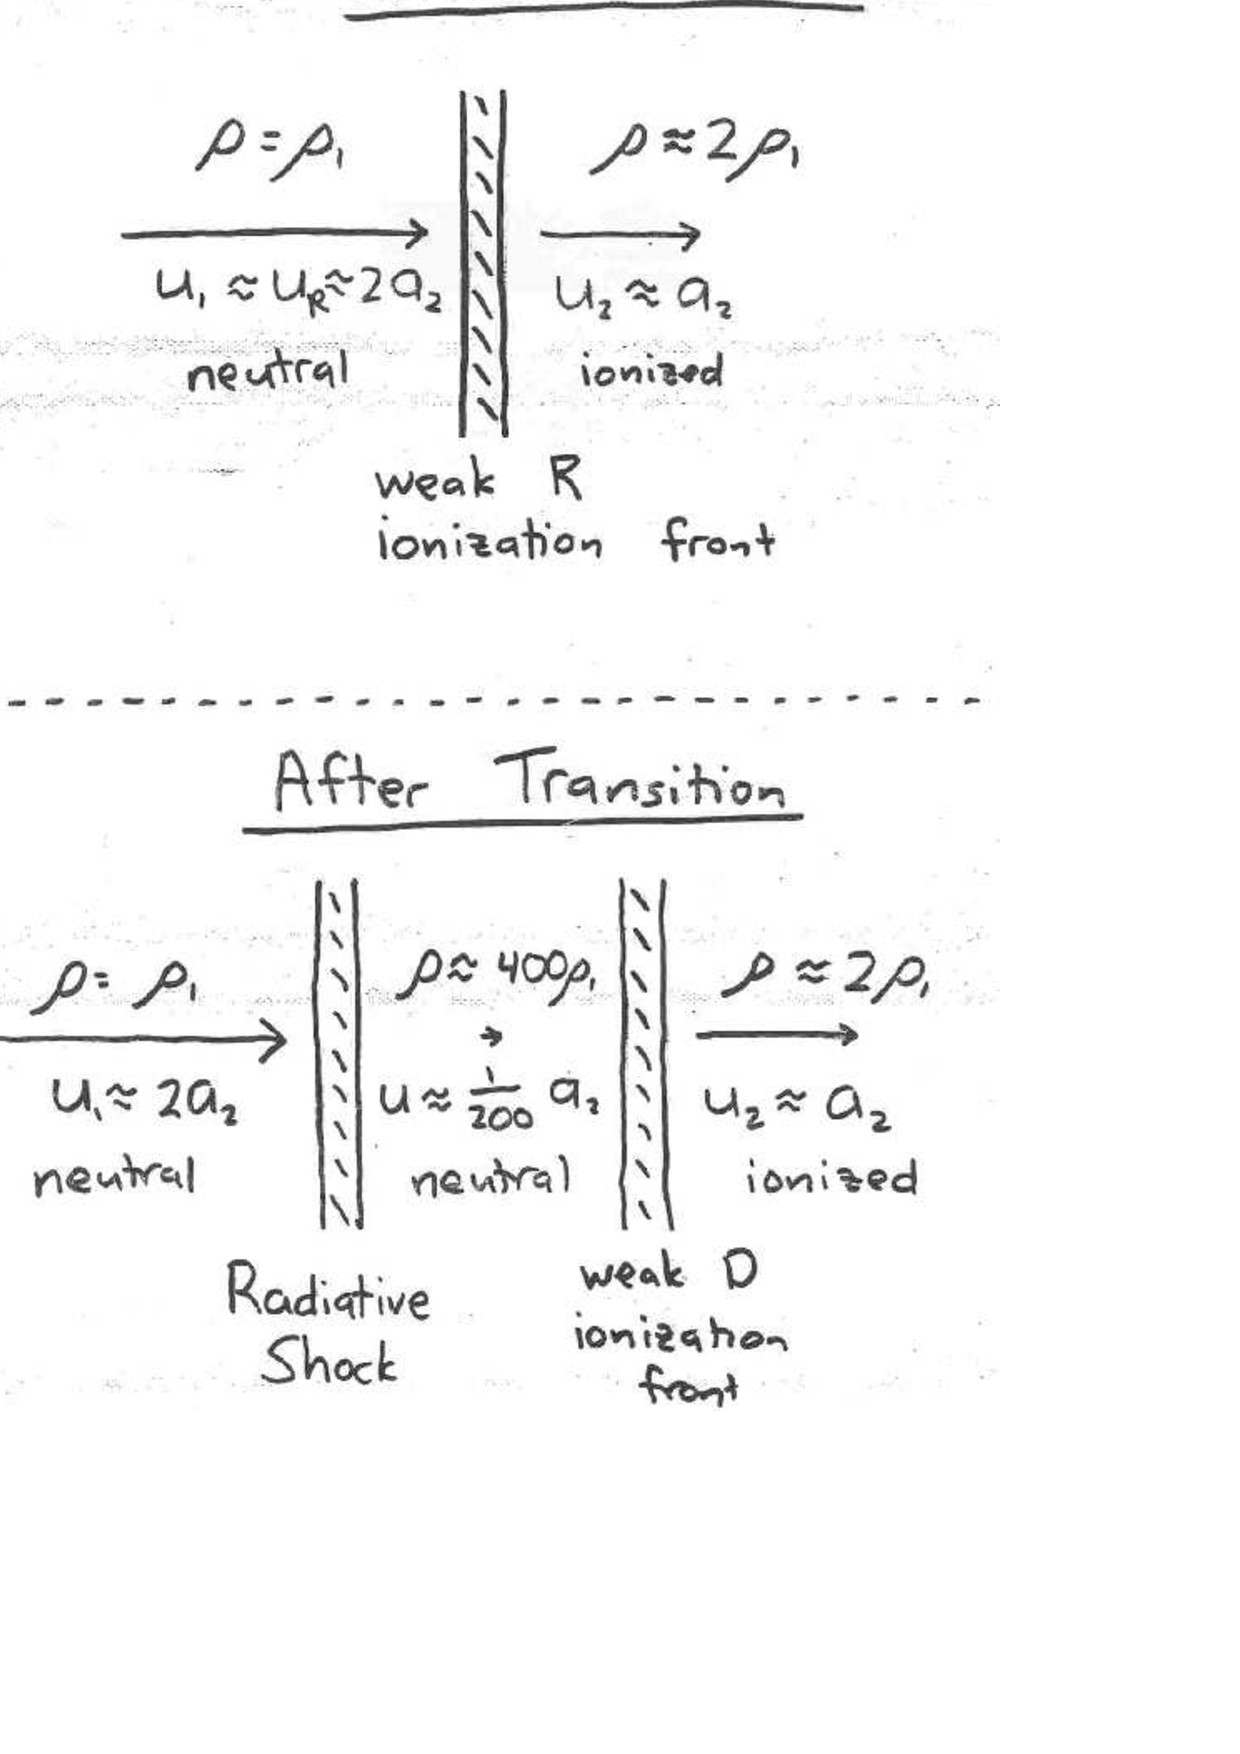
\includegraphics[width=\textwidth]{shock_diagram.pdf}
\end{center}
\caption{Evolution of the shock created by an expanding HII region \label{fig:front}}
\end{figure}

The other thing of interest for HII regions is ionization fraction.  Balancing ionization with 
recombination gives
\begin{equation}
n_{photon}n(1-x)\sigma_{i}c=\alpha x^2n^2
\end{equation}
where x is the fraction of ionized H and n is the total number density of the gas.  The number 
of photons per second coming from the star pass through a volume $4\pi R^2c$, so 
\begin{equation}
n_{photon}=\frac{Q_*}{4\pi r^2c}
\end{equation}
Solving for x and plugging in typical HII region values gives over 99\% ionization (Nutshell 
has an example where $x=0.999983$).  

Also, it might be good to know that the outer parts of an HII region are hotter than the inner 
parts.  This is because the photons that make it to the outer region have a harder spectrum, so 
they can heat the gas more efficiently.  The cross section for H ionization decreases as 
$\nu^{-3}$, so lower energy photons do most of the ionization inside the region.  By the time 
photons reach the outer parts, the lower energy photons have been used up.  

\subsection{Dust}
Dust is formed in the outer layers of AGB stars.  Simple molecules involving 
C or O (depending on the composition of the star) form first.  When the outer 
layers of the star cool to around $1000$ K, gas phase molecules condense onto 
these SiC and SiO seeds, forming more complicated dust molecules.  Based on 
spectra, it is estimated an AGB star ejects $\sim10^8\ M_{\odot}$ of dust 
per year, meaning in the entire galaxy, $\sim10^{-2}\ M_{\odot}$ of dust 
are put into the ISM by AGB stars every year.  

Dust can be destroyed or altered by UV radiation or cosmic rays, as well 
as things like shocks, nearby stars turning on, or anything else that can heat 
interstellar clouds.  For example (we don't actually need to know this, but 
it's hilarious, so I'm including it), lab experiments show that simple ices 
exposed to UV radiation and warmed form an organic ``yellow stuff'' (that's the 
scientific term, check Kwok, it's even in the index!).  When the yellow stuff 
is taken into space and exposed to solar radiation, it turns brown (might I 
suggest another scientific term- ``gets a tan'')

Some facts about dust:

Thermal emission from dust grains is usually in the range of sub-mm wavelengths 
to about $2~\mu m$. Interstellar grains, with temperatures of $10-100$ K, emit
at $30-300\ \mu$m.  Grains near stars have temperatures of a few hundred 
Kelvin, and emit at around $10\ \mu$m.  Dust extinguishes (through both absorption and scattering) background sources in the $0.1-20~\mu m$ range, from UV to mid-IR. This range implies that the sizes of particles is about $0.1-0.2~\mu m$, though I'm not sure why. Dust also polarizes light, and this has to do with how magnetic fields cause dust grains to align, but someone should help fill in the details here.

Some observational evidence of dust includes the following. One is that low observed abundances of heavy elements, i.e. lower than solar, means that individual metal atoms have been depleted in order to form dust grains. Another is the presence of molecular hydrogen, whose formation if catalyzed on the surfaces of dust grains. Dust also can shield H$_2$ from UV radiation, which prevents it from dissociating as much (Anneila also lists IR absorption lines and diffuse radiation in the galaxy. See notes 5).

Scattering by dust roughly follows a $\lambda^{-1}$ law, meaning that redder light is extinguished more easily. Extinction from dust, represented by $A_\lambda$, increases the apparent magnitude of an object:

\begin{equation}
m_\lambda = M + 5 \log d - 5 + A_\lambda \,\, .
\end{equation}

Assuming $I = I_0 e^{-\tau_\lambda}$,

\subsection{Phases of a Supernova}
\newthought{Anneila mentioned that} this was a fairly popular question on the quals, so
I believe a brief review of the phases of a supernova is relevant.  This focuses on the
supernova remnant as opposed to the supernova mechanism itself.  Please edit this if I wrote
something that is wrong or could be explained better -- this is the point of using git.
\begin{enumerate}
    \item The free-expansion phase

    This phase is defined by the fact that the velocity of the ejecta is constant with time. This is also known as ``homologous expansion" because the shape of the density profile remains the same. For every shell of the expanding ejecta, the distance from the source $r = vt$. The condition for being in this phase is that $M_{\rm ejecta} \gg M_{\rm swept}$, that is, the mass swept up by the ejecta from the ISM is not a significant fraction of the ejecta mass.
    The expanding mass of ejecta creates a shock that travels outwards through the ISM
    and a reverse shock that travels inwards through the ejecta.  The reverse shock has a finite
    amount of material to travel through and dies away.
    The outward traveling shock heats the ISM behind it to very high temperatures.
    Thermal bremsstrahlung is seen
    in X-rays, and synchrotron emission is seen in radio from ejected
    particles spiralling around $\mu$G magnetic fields.  This phase ends after 10s to 100s of
    years when the mass of the swept up from the ISM is comparable to the mass of the ejecta.
    Recall that high-mass stars (the progenitors of core-collapse supernovae) typically
    drive large stellar winds.

    \item The adiabatic phase (also called Sedov-Taylor or Blast Wave phase)

    In this phase, the mass of the swept up ISM dominates the mass of the ejected material ($M_{\rm swept} > M_{\rm ejecta}$).
    However, the density of the material behind the shock is not yet large enough for cooling
    to be significant.  Therefore, the gas expands adiabatically.
    From dimensional analysis considerations, we can derive the Sedov-Taylor solution which says
    \begin{dmath}
        R \sim \left(\frac{Et^2}{\rho}\right)^{1/5}
    \end{dmath},
    where $R$ is the radius of the supernova remnant, $E$ is the energy released by the
    supernova, and $\rho$ is the density of the surrounding ISM. The Sedov phase usually lasts about $10^4$ years.

    \item The radiative phase (or snowplow phase)
    
    This is also called the momentum-conserving phase. Consider a shell with mass $M_s$ and velocity $v_s$. The momentum $p_0 = M_s v_s$ is constant, giving the equation of motion
    \begin{equation}
    p_0 - \biggl(\frac{4}{3}\pi R^3 \rho_0 \biggr) \dot{R}\,\, ,
    \end{equation}
    which can be integrated to show that
    \begin{equation}
    R \propto t^{1/4}\,\,.
    \end{equation}
    \item Merger with the ISM
    
    Occurs when $v_s = c_s$ is the sound speed.
\end{enumerate}

\subsection{The Fluid Equations}
The following are the ideal or ``inviscid" fluid equations.

Mass conservation:
\begin{equation}
\frac{\partial \rho}{\partial t} + \vec{\nabla} \cdot \rho \vec{v} = 0
\end{equation}

Momentum conservation:
\begin{equation}
\frac{\partial}{\partial t} (\rho \vec{v}) + \vec{\nabla}\cdot (\rho \vec{v} \vec{v}) = -\vec{\nabla} P + \rho \vec{f}
\end{equation}

Energy conservation:
\begin{equation}
\frac{\partial}{\partial t} \biggl( \frac{1}{2} \rho v^2 + \rho \epsilon \biggr) + \vec{\nabla}\biggl[\biggl(\frac{1}{2}\rho v^2 + \rho \epsilon \biggr) + P \vec{v} \biggr] = \rho \vec{f} \cdot \vec{v}\,\,.
\end{equation}
The right-hand side of this equation is the work done by external forces (other people should feel free to add to this section or add different forms of the equations). Also, the Lagrangian or ``comoving" time derivative is

\begin{equation}
\frac{d}{dt} = \frac{\partial}{\partial t} + (\vec{v} \cdot \vec{\nabla})\,\, ,
\end{equation}
where $\frac{\partial}{\partial t}$ is the Eulerian time derivative, not comoving with the fluid.

It's probably good to know basically how to do perturbation theory on these equations, which you can do by saying $\rho \rightarrow \rho_0 + \delta \rho$ and the same with $P$ and $v$ (assume $v_0 = 0$), then killing all the terms that are second-order in $\delta$ quantities.

It's also a good idea to know Bernoulli's equation:
\begin{equation}
(\vec{v}\cdot \vec{\nabla})\biggl(\frac{1}{2} v^2 + h + \phi \biggr) = 0\,\, .
\end{equation}
or
\begin{equation}
\frac{1}{2} v^2 + h + \phi = {\rm constant}
\end{equation}
along every streamline. The first term is kinetic energy, the second is gravitational potential energy, and and third is thermal energy $+$ work that can be done.

\subsection{Shocks}
Adiabatic shocks:\newline
Shocks form easily in astrophysical enviroments because gravity can accelarate 
gas to large velocities, but the cold gas in the ISM has a low sound speed.  
The ratio of flow velocity to sound speed is called the Mach number:
\begin{equation}
\boxed{M=\frac{v}{c_s}}
\end{equation}
A shock forms when the bulk flow of a fluid is faster than the sound speed in the 
gas, and the gas is decelerated by another fluid.  Since the fluid is 
moving supersonically, the next layer of the fluid hits the decelaration before 
information about the decelaration can reach it from the previous layer.  So 
the fluid cannot adjust slowly to the decelaration, and a discontinuity forms.  
This is a shock.  

Adiabatic Shocks:\newline
The jump conditions across a shock can be derived using the 1-D fluid 
continiuity equations across the shock boundary.  In the frame of the shock, 
fluid is coming at the shock from region 1 and leaving the shock into region 2.  
Consider a thin layer d$x$ around the shock.  Starting with mass continuity:
\begin{equation}
\frac{\partial \rho}{\partial t}+\frac{\partial}{\partial x}(\rho u_x)=0
\end{equation}
Mass is not accumalted in the layer d$x$, so 
$\frac{\partial \rho}{\partial t}=0$.  This implies 
$\frac{\partial}{\partial x}(\rho u_x)=0$, so 
\begin{equation}
\boxed{\rho_1u_2=\rho_2u_2}
\end{equation}
Similarly, the momentum energy conservation equations (assuming an adiabatic 
shock) give 
\begin{equation}
\boxed{\rho_1u_1^2+p_1=\rho_2u_2^2+p_2}
\end{equation}
\begin{equation}
\boxed{\frac{1}{2}u_1^2+\epsilon_1+\frac{p_1}{\rho_1}=\frac{1}{2}u_2^2+\epsilon_2+\frac{p_2}{\rho_2}}
\end{equation}
These are the Rankine-Hugoniot jump conditions.  The energy condition can 
be put into a more convenient form by substituting for $\epsilon$, the internal 
energy per unit mass.  The fluid is brought to $\epsilon$ by $p$d$V$ work (it's 
adiabatic), so
\begin{equation}
\epsilon=\frac{pdV}{m}=K\rho^{\gamma}d(1/\rho)=\frac{1}{\gamma-1}\frac{p}{\rho}
\end{equation}
Then
\begin{equation}
\frac{1}{2}u_1^2+\frac{\gamma}{\gamma-1}\frac{p_1}{\rho_1}=\frac{1}{2}u_2^2+\frac{\gamma}{\gamma-1}\frac{p_2}{\rho_2}
\end{equation}
Assuming $\gamma$ does not change across the shock.  Using 
$=\gamma\frac{p}{\rho}$,
\begin{equation}
\frac{1}{2}u_1^2+\frac{c_1^2}{\gamma-1}=\frac{1}{2}u_2^2+\frac{c_2^2}{\gamma-1}
\end{equation}
Now follows a bunch of messy algebra that we probably don't need to know, but 
look at pages 82 and 83 of Clark and Carswell if you're interested.  
The result is that 
\begin{equation}
\frac{\rho_2}{\rho_1}=\frac{(\gamma+1)p_2+(\gamma-1)p_1}{(\gamma+1)p_1+(\gamma-1)p_2}
\end{equation}
In a strong shock, $p_1$ is negligible, and this expression becomes
\begin{equation}\label{eq:den}
\boxed{\frac{\rho_2}{\rho_1}=\frac{\gamma+1}{\gamma-1}=4}
\end{equation}
assuming $\gamma=5/3$.  The compression of the fluid is limited because of 
the adiabatic assumption.  As the shock gets stronger, the thermal pressure 
of the post-shocked gas increases, which prevents additional compression.  
If the thermal energy could be released, this wouldn't happen, but we assumed 
the shock is adiabatic.  

Using the second jump condition, and neglecting $p_1$, 
\begin{equation}
P_2=\rho_1u_1^2-\rho_2u_2^2=\rho_1u_1^2-\rho_1u_1^2/4=\frac{3}{4}\rho_1u_1^2
\end{equation}
This can be used with Equation \ref{eq:den} and the ideal gas law to show 
\begin{equation}
\boxed{T_2=\frac{3\mu m_H u_1^2}{16k}}
\end{equation}
For typical shock velocities of $100$ km/s, this corresponds to post-shock 
temperatures of $\sim10^5$ K.  Also of interest is the Mach number of the 
post-shocked gas.  
\begin{equation}
M_2^2=\frac{u_2^2}{c_2^2}=
\frac{\rho_2}{\gamma p_2}\frac{u_1^2}{16}=
\frac{u_1^2}{16}\frac{4\rho_2}{3\gamma\rho_1u_1^2}=
\frac{1}{3\gamma}=
\frac{1}{5}
\end{equation}
So the post-shocked gas moves subsonically.

Isothermal Shocks:\newline
The other limiting case of shocks is an isothermal shock.  In an isothermal 
shock, the shocked gas cools to its pre-shock temperature.  This 
happens over a cooling length that is much less than the lengthscale of the 
system.  The immediate post-shock will be adiabatic, but if this is over a 
small enough length, the adiabatic portion can be lumped is as part of the 
shock and ignored.  The continuity conditions can then be applied to the 
pre-shock and isothermal part of the post-shock.  The first two jump conditions 
still hold, but the energy conserving one no longer applies.  Instead, it is 
replaced by 
\begin{equation}
\boxed{T_1=T_2}
\end{equation}
Since the shock is isothermal, the sounds speed before and after is the same.
\begin{equation}
c_s^2=\frac{p}{\rho}
\end{equation}
The momentum jump condition then gives
\begin{equation}
\rho_1(u_1^2+c_s^2)=\rho_2(u_2^2+c_s^2)
\end{equation}
Substituting the mass jump condition for $\rho_1$ and rearrangeing gives
\begin{equation}
(u_2-u_1)c_s^2=u_1u_2(u_2-u_1)
\end{equation}
Therefore
\begin{equation}
c_s^2=u_1u_2
\end{equation}
and 
\begin{equation}
\boxed{\frac{\rho_2}{\rho_1}=\frac{u_1}{u_2}=\left(\frac{u_1}{c_s}\right)^2=M^2}
\end{equation}
So there is no limit to how much a strong shock can compress the gas.  
Note that because $c_s^2=u_1u_2$ and $u_1>c_s$ by definition of a shock, the 
post-shocked gas is subsonic.  

Magnetic Fields in Shocks:\newline
This is based on the class notes, so I'm going to be making some statements 
that seem to come out of thin air (just like they do in the notes).  Someone 
who has a better reference or understands this better should fill in the 
details.  

In the presence of magnetic field, magnetic pressure must be included in 
the momentum conservation equation across a shock of a plasma.  
\begin{equation}
P_1+\rho_1v_s^2+\frac{B_1^2}{8\pi}=P_2+\rho_2u_2^2+\frac{B_2^2}{8\pi}
\end{equation}
Assuming that in the pre-shock gas, ram pressure dominates and in the post-
shock gas, magnetic pressure dominates, this becomes
\begin{equation}\label{eq:B2}
B_2^2=8\pi\rho_1v_s^2
\end{equation}
Because the magnetic field lines are frozen into the plasma and magnetic flux 
$B/\rho$ is through a ``circuit'' of the plasma is conserved, the presence 
of the magnetic field reduces the compression of the gas by the shock.  
By flux conservation:
\begin{equation}
B_2=B_1\frac{\rho_2}{\rho_1}
\end{equation}
Combining this with Equation \ref{eq:B2} and solving for the density ratio gives
\begin{equation}
\left(\frac{\rho_2}{\rho_1}\right)^2=2\times\frac{4\pi\rho_1v_s^2}{B_1^2}=2\frac{v_s^2}{v_a^2}
\end{equation}
where $v_a$ is the \emph{Alfven velocity}, defined as
\begin{equation}
v_a\equiv\frac{B}{(4\pi\rho)^{1/2}}
\end{equation}
The Alfven Mach number is then defined as 
\begin{equation}
M_A\equiv\frac{v_s}{v_A}
\end{equation}
With this definition, 
\begin{equation}
\frac{\rho_2}{\rho_1}=\sqrt{2}M_A
\end{equation}
In the presence of a magnetic field, disturnbance propogate at the Alfven 
velocity, not at the sound speed.  

In a gas containing a mix of ions and neutrals, a magnetic field will affect 
the structure of a shock.  Only the ions feel the magnetic field, but they 
can transfer the effects to the neutrals through collisions.  The shock 
structure depends on the strength off the magnetic field.  A magnetic 
precursor to the shock with smooth out the velocity disontinuity for the ions 
(see Figure \ref{fig:Cshock}).  The magnetic field does not want to 
suddenly change strength (and therefore flux), so it pushes the ions away from 
the shock, smoothing their velocity and density change into the shock.  
In a very weak magnetic field, the ions will 
have a small warning off the shock, and will feel less of a discontinuity, 
while the neutrals will be uneffected and feel a normal \emph{J-shock}.  For 
increasingly strong magnetic fields, the ions will have more warning and 
their discontinuity will be increasingly smoothed out.  With the additional 
warning time, the ions will have more time to collisionally change the 
neutral velocity, smoothing out the neutral discontinuity as well.  If the 
magnetic field is strong enough, the J-shock of the neutral will turn into 
a completely smooth transition known as a \emph{C-shock}.

\begin{figure}[!h]
\begin{center}
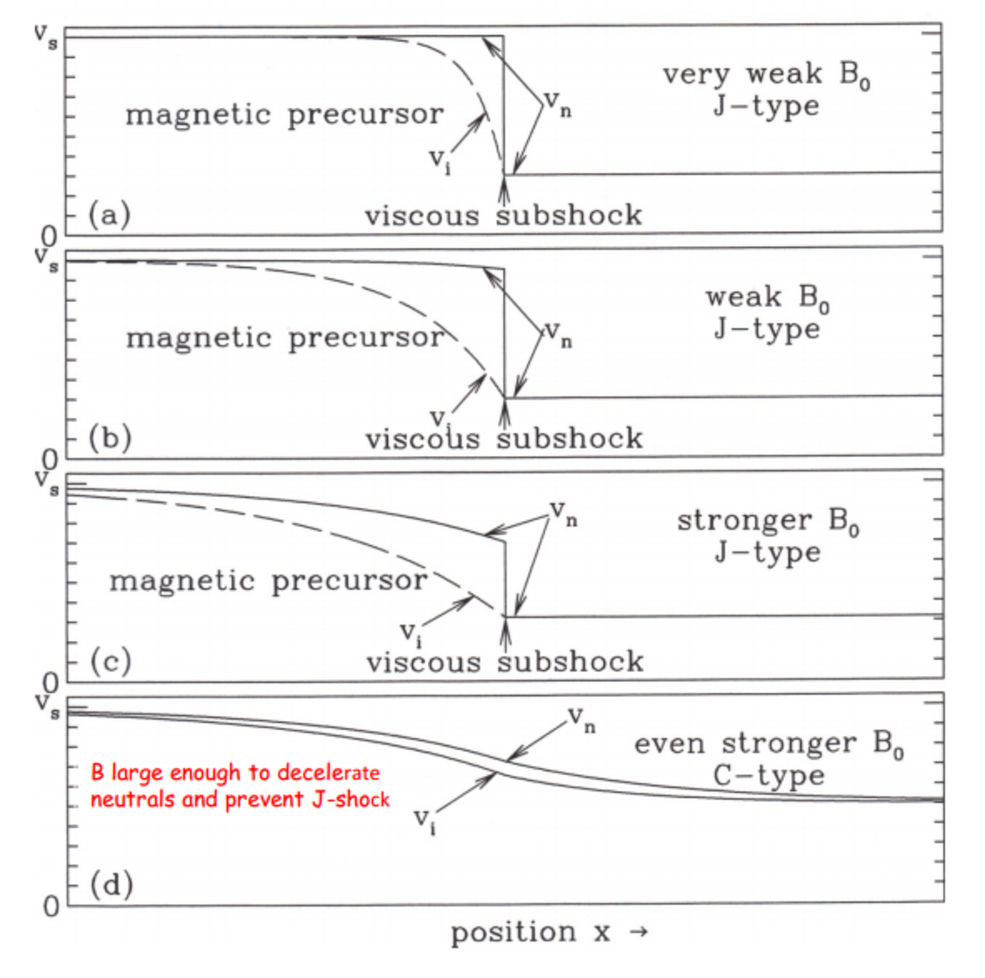
\includegraphics[width=\textwidth]{Cshock.pdf}
\end{center}
\caption{Shocks involving magnetic fields. \label{fig:Cshock}}
\end{figure}

\subsection{Magnetic Fields}
Applications of magnetic fields is covered in shocks and in star formation.  

Observational evidence of interstellar magnetic fields include polarization 
of starlight, the Zeeman effect, and pulsar faraday rotation measurements.  
Polarization of starlight is caused by non-sherical dust grains.  These dust 
grains can be modeled as cylinders rotating end over end, with their short 
axis parallel to the B field.  Observations indicate ISM B fields of order 
$10^{-6}$ gauss.  The Zeeman effect can be observed as hyperfine splitting 
of the $21$ cm H line due to the B field.  The frequency difference between 
the two lines is $\frac{eB}{4\pi m_ec}\sim3\times10^6B Hz$, so this is 
difficult to observe for B fields of $10^{-6}$ gauss.  

Faraday rotation is the rotation of linearly polarized light to a different 
linear polarization as it passes through a plasma with a magnetic field going 
through it (see section in radiative processes).  The amount of rotation, which 
can be measured as a function of frequency, is 
$\propto \int_0^L n_eB$, so a measure of rotation gives the product of density 
and magnetic field.  The density can be determined using dispersion, a measure 
of the time delay in a signal as a function of frequency.  This is proportional 
to $\int_0^L n_e$.  So by measuring Faraday rotation and dispersion, B can 
be determined.  Pulsar observations using this technique find a B field 
strength also of order $10^{-6}$ gauss. 

\subsection{Star Formation}
I think most of what we need to know about star formation is in the Stars 
section of the notes.  The only thing new here is magnetic fields.  

Most molecular cloud cores are Jeans-unstable to collapse, but star formation 
efficiency is lower than it should be if this is true.  The angular momentum 
and magnetic flux in stars is lower than that in clouds, so angular momentum 
and magnetic flux must be lost during collapse.  Also, collapsing clouds are 
not as flat as theory predicts, and have broadened lines implying some sort 
of turbulence.  All this implies magnetic fields play an important role in star 
formation.  \emph{Ambipolar diffusion} delays cloud collapse and provides a way 
for magnetic flux to be lost.  The Alfven waves produced in this process 
cause turbulence, which can broaden spectral lines (the notes just state these 
things without justifying them).   

Even in a cold molecular cloud core, this is a small fraction of ionization.  
The ionized particles are frozen to the magnetic field lines, which prevents 
them from collapsing.  The neutral particles don't care about the magnetic 
field lines, but they do have diffuse through the trapped ions in order to 
collapse.  The force per unit volume $f$ on the neutrals from collions with the 
ions is the collision rate per unit volume times the change in momentum 
of a neutral per collision.  So $f$ is given by
\begin{equation}
f=n_in_n<v\sigma>m_n(u_i-u_n)
\end{equation}
Here, $u_i-u_n$ is the velocity of the neutrals relative to the ions and field 
lines.  Therefore, this is also the velocity with which the neutrals drift 
across the magnetic field lines, $v_D$.  Balancing the collisional force with 
gravity:
\begin{equation}
\rho\frac{GM}{r^2}=n_in_n<v\sigma>m_nv_D
\end{equation}
\begin{equation}
n_nm_n\frac{GM}{r^2}=n_in_n<v\sigma>m_nv_D
\end{equation}
\begin{equation}
\frac{GM}{r^2}=n_i<v\sigma>v_D
\end{equation}
The left hand side can be rewritten as
\begin{equation}
\frac{GM}{r^2}=\frac{GM}{r^3}r=\frac{4\pi}{3}Gn_nm_nr
\end{equation}
So
\begin{equation}
\frac{4\pi}{3}Gn_nm_nr=n_i<v\sigma>v_D
\end{equation}
\begin{equation}
v_D=\frac{4\pi}{3}\frac{Gn_nm_nr}{n_i<v\sigma>}
\end{equation}
The timescale for ambipolar diffusion is 
\begin{equation}
t_D=\frac{r}{v_D}=\frac{3n_i<v\sigma>}{4\pi Gn_nm_n}\sim7\times10^{13}\frac{n_i}{n_n} years
\end{equation}
I'm not sure where the numbers being plugged into this come from.  For 
molecular cloud cores, $n_i/n_n\lesssim10^{-6}-10^{-5}$, so the diffusion time 
is $\lesssim10^7$ years.

\subsection{ISM in Other Galaxies}
The following is taken from slide 21 on February 28.  I don't really understand 
it, but it get's an entire slide to itself, so it must be important...

AGN       ?'s.....

The other galaxies stuff is all from Nick's slides, so most of what he 
shows is example spectra and images.  Not really sure what to do with that, 
but he's on the committee and this is what he does research on, so he might 
ask about it.  If anyone has a better reference for this stuff, feel free 
to add to this section.  The main topics seem to be special types of galaxies 
like AGN and galaxies with lots of star formation.  AGN will be covered in High Energy with better detail, 
so I'll skip that for now.  

Star formation happens in starburst galaxies, where a recent galaxy merger 
forces large amounts of gas into the center, triggering star formation.  
If the star formation is obscured by dust, the dust re-emitts at longer 
wavelengths and you see an ULIRG (Ultra-Luminous Infrared Galaxy) or a sub-mm 
galaxies.  This is about all I know off the top of my head, and I can't figure 
out anything useful from Nick's notes.  I think this topic is partially covered 
in the Galaxies will-ask though, and may also be covered in George's cosmology 
topics.  

\section{Cosmology}
\subsection{Questions}
\begin{enumerate}
\item Put on a timeline, and describe the principal events in the thermal history of the
universe, from $kT = 10$ TeV to $kT = 0.1$ eV.
\item Give a semi-quantitative discussion of the connection between flucuations of the
cosmic microwave background on angular scales of arcminutes to degrees, and the
baryonic structures (galaxies, clusters, correlations of galaxies) observed in the local
universe, redshift $z < 0.5$.
\item Which elements/isotopes are produced in Big Bang Nucleosynthesis and in what
quantities? Explain qualitatively how the yield of each depends on the cosmic baryon
density and why.
\end{enumerate}

\subsection{What Distance Means in Cosmology}

\subsection{Measuring Distances}\label{sec:distance_ladder}
The basic concept of distance is the distance ladder, which is basically 
different techniques used to measure distances farther and farther away.  
There is overlap between the different techniques, which allows the next 
technique to be calibrated by the previous one.  The only problem with this 
is errors and uncertainties at the bottom of the ladder propogate all the 
way up.  

The first step is parallaxes, which are reliable out to $\sim100$ pc or so.  As 
the Earth moves around the Sun, the apparent positions of stars will change 
slightly relative to more distant fixed background stars.  The distance 
to an object in parsecs is defined to be $\frac{1}{p}$ where $p$ is the 
parallax in arcseconds.  One useful trick to know for quickly converting 
between angular size and physical size- the physical size in AU of something 
$d$ parsecs away with an angular size of $\theta$ arcsec is just $\theta d$.  
So, for example, if a star and planet are $1$ pc away and are separated by 
$1$ arcsec, the planet is $1$ AU from the star.  Parallax is the only 
distance indicator that is not model dependent or reliant on some other 
calibration.  

Out to distances of $\sim1$ kpc, main sequence fitting can be used to find 
distances to main sequence stars.  If the spectral type of a star is measured, 
and the absolute magnitude of that spectral type is known from a closer 
star with a parallax distance, the difference between apparent and absolute 
magnitude gives the distance to the new star.  

This has been done for clusters of stars that contain Cepheid variables, 
leading to the next step in the distance ladder.  Cepheids are horizontal 
branch high mass stars in the instability strip of the HR diagram (see Stars 
notes).  Cepheids are useflu as distance indicators because their periods 
are tightly correlated with their luminosities by 
\begin{equation}
\log{\frac{L}{L_{\odot}}}\sim2.4+1.2\log{\frac{P}{days}}
\end{equation}
So by measuring the period of pulsation, the intrinsic luminosity can be 
determined, giving a distance.  Nearby galaxies (within $20$ Mpc) are close 
enough that individual Cepheids can be observed and used to get distances.  

Advantages:  Bright ($M_V\sim-4$ to $-7$), so the can be used in other galaxies.  
Also, we understand the physics behind their pulsation well, and can identify 
them based on their period.  

Disadvantages:  Cepheids are relatively rare since they correspond to short 
phases of stellar evolution and high masses.  Also, there are uncertainites 
about systematics of the period-luminosity relation like how it depends on 
metallicity and color.  

The tip of the red giant branch method is applicable out to similar distances 
as Cepheids.  Stars at the top of the red giant branch, right before He flash, 
have a known absolute magnitude of $-4$.  This point also corresponds to a 
drop-off in the frequency of stars, so once this is found and its brightness 
is measured, the distance can be determined.  

Advantages: Stars are bright and method is relatively precise and 
well-understood.  

Disadvantages:  Only works for old populations.  

Another method is planetary nebulae luminosity functions.  Planetary nebulae 
have an observed cut-off in luminosity at absolute magnitude $-4.5$.  The 
physics behind the cut-off is understood, and planetary nebulae can be found 
in all types of galaxies.  

For galaxies out to $\sim100$ Mpc, there are several methods to get distances, 
including the Tully-Fisher relation, globular cluster  
luminosity functions, and surface brightness fluctuations.  The Tully-Fisher 
relation is an observed correlation between the rotational velocity of 
spiral galaxies and their luminosity:
\begin{equation}
L\propto v_{rot}^4
\end{equation}
The rotational velocity is usually measured by HI $21$ cm line width.  The 
problems with this method are the relation has $\sim10-20$\% scatter, and 
the physics behind it are not well understood.  The fundamental plane gives 
similar relations for elliptical galaxies.  Globular clusters have well-defined empirical luminosity functions that can be used as 
standard candels.  Globular clusters have a peak at an absolute magnitude 
of $-6.6$.  An advantage of this method is it is not affected by dust.  
However, deep photometry is needed to measure the luminosity function, and 
this method is not as precise as others.  Surface brightness fluctuations 
involve measuring the surface brightness (flux per solid angle) in several 
regions of the same galaxy.  The observed surface brightness depends on the 
number of stars in the region, which should be similar in the different 
patches.  If the average number of stars is N, the Poisson scatter in the 
number of stars (and thus the brightness) will be $\frac{1}{\sqrt{N}}$.  
The number of stars per solid angle will also depend on distance as 
$N\propto r^2$.  So the observed scatter $\sigma\propto\frac{1}{r}$.  This 
relation can be calibrated using nearby galaxies.   

For even more distant galaxies (out to $\sim1$ Gpc), Type Ia supernovae 
can be used as standard candles to get a distance.  A tight correlation 
exists between the shape of a Ia lightcurve and the luminosity of the 
supernova, so by measuring the shape of the light curve, the distance can 
be determined.  This method is very precise, but we still don't understand 
the mechanism for a type Ia supernova.  Type Ia supernovae can be observed 
into the Hubble flow, so a plot of distance versus redshift can be used 
to determine the cosmological parameters.  The main problem with all these 
methods so far is they rely on calibrations from other methods.  One of the 
main goals of the Hubble Space Telescope was to improve these calibrations 
and determine $H_0$ more precisely.  The main focus was to better calibrate 
Cepheids and the distance to the LMC and SMC, which other methods are based 
on.  The HST $H_0$ Key Project determined $H_0=72\pm3\pm7$ km/s/Mpc.

Two methods that don't need calibration, but instead are model dependent 
are the S-Z effect (see section in Radiative) and gravitational lense 
time delays.  If a background quasar is lensed, variability in the quasar 
will be seen at different times on different sides of the lense, since the 
path length is different.  If the mass distribution of the lense is known, 
then the ratio of the path length difference to the source distance and lense 
distance can be determined.  Since the time delay is known, the path length 
difference can be calculated, giving the distance to the lense and the 
background quasar.  The modeling is very complicated however.  

\subsection{Age of the Universe}
An estimate of the age of the Universe is the Hubble time 
$t_H=1/H_0=4.4\times10^{17}h_{70}^{-1}$ s.  The exact age depends on the other 
cosmological parameters.  Other methods to get a lower limit on the age include 
globular cluster ages, white dwarf cooling times, and nucleocosmochronology 
(that's a mouthful).  Globular clusters are some of the oldest objects 
we can observe, so their ages give good lower limit to the age of the 
Universe.  The observed main sequence turnoff of a globular cluster can be 
combined with stellar isochrones to determine an age.  Uncertainties in 
the isochrone models and the distances to the clusters complicate this, 
but this methods gives lower limits ranging from around $10$ to $15$ Gyr.  
White dwarfs can also be used to age date globular clusters.  Higher 
mass stars turn into white dwarfs after only a few tens of Myr, so the 
white dwarfs will be $\sim$the same age as the cluster.  White dwarfs cool 
as they age in a fairly well understood way, so the luminosity of the 
dimmest white dwarfs in a cluster gives the age of the cluster.  There are 
still uncertainties in the cooling models though, and these white dwarfs are 
extremely faint, so this has only been done for one cluster, but the age 
agrees with the main sequence turnoff age.  Measuring abundance ratios of 
radioactive elements with Gyr or 10 Gyr half lives can also provide an estimate 
of the age.  This is difficult because the lines of these elements tend to be 
very weak in stars, but the measurements made so far give ages in the range of 
about $10-15$ Gyr.  All these methods are in agreement with the age determined 
from cosmological parameters.  

\subsection{Expansion of the Universe Tests}
Tolman Test:\newline
Observe something with a uniform surface brightness at different redshifts.  
Surface brightness is just flux per unit solid angle, so 
\begin{equation}
B=\frac{f}{d\Omega}
\end{equation}
\begin{equation}
B=\frac{L}{D_L^2}\frac{D_A^2}{dl^2}
\end{equation}
In a Euclidean, non-expanding Universe, $D_L=D_A$, so surface brightness should 
be constant for objects of constant $L/dl^2$.  In an expanding Universe, 
$D_L=D_A(1+z)^2$, so $B\propto(1+z)^{-4}$.  The intercept of the surface 
brightness scaling relations for elliptical galaxies make a good standard 
surface brightness.  Observations of clusters at different redshifts match 
$B\propto(1+z)^{-4}$.  

Hubble Diagrams:\newline
Hubble diagrams use standard candels or standard rulers to plot luminosity 
distance or angular diameter distance vs. redshift.  The shape of the 
curve gives information about the cosmological parameters.  For example, 
if the Universe has a lower density or positive $\Lambda$, it will have 
expanded faster and be larger today.  We know the Hubble constant today, 
so to slow down to this expansion rate would require more time, so the 
Universe would be older.  Since the Universe is larger, at a given 
redshift, objects would be further away, so they would look fainter and 
smaller.  A higher density Universe would behave the opposite way.  Plots 
of luminosity/angular diameter distance (or some proxy like magnitude or 
angular size) vs. redshift would show this (see Figure \ref{fig:hubble}).

\begin{figure}[!h]
\begin{center}
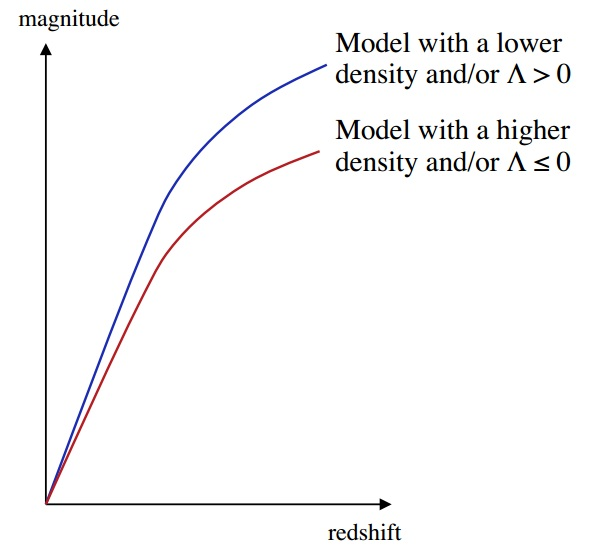
\includegraphics[width=\textwidth]{hubble.jpg}
\end{center}
\caption{A Hubble Diagram for different cosmological parameters.
\label{fig:hubble}}
\end{figure}

Early attempts at this used galaxies, clusters, and radio sources as standard 
candles and standard rulers, but galaxy and cluster evolution effects 
dominated over the effects of different cosmologies.  The use of type Ia 
supernovae (standard candles) and CMB fluctuations (standard rulers) provided 
much better tests.  

In these tests, biases from missed sources must be taken into account, as well 
as the K correction.  The idea behind the K correction is if we measure the 
light from a galaxy in a certain bandpass in our frame, the light we are seeing 
is from a bluer region of the spectrum, and this region is narrower by a 
factor of (1+z).  The bandpass emitted by the galaxy is redshifted and 
stretched when it reaches us.  This effect depends on redshift, so it must be 
taken into account when looking at galaxies at different redshifts.  The 
ratio of the flux in our frame to the flux in the galaxy's frame as a function 
of redshift has been computed for different types of galaxies and for different 
bandpasses.  

Using type Ia supernovae or CMB fluctuations indivually creates a degeneracy 
between $\Omega_{\Lambda}$ and $\Omega_M$ (here, $\Omega_M$ is density of 
baryonic and dark matter).  Combining these tests, however, breaks the 
degeneracy, and results in $\Omega_{\Lambda}\sim0.7$ and $\Omega_M\sim0.3$.

Another cosmological test is galaxy and cluster counts.  Plotting 
source counts vs magnitude (as a proxy for redshift) gives information 
on the density of the Universe.  A Universe with lower denstiy or higher 
$\Lambda$ will be larger, therefore there will be more sources to observe, 
so the curve will be higher.  A Universe with higher density will be smaller, 
and have a lower curve.  Galaxy evolution makes things difficult.  Galaxies 
were brighter in the past, so there will be extra counts at brighter 
magnitudes.  Also, because galaxies merge, there were more faint pieces in 
the past, which produces extra counts at fainter magnitudes.  To avoid this, 
really need redshifts of these galaxies.  Cluster counts rely on the 
assumption that we know what the number density of distant clusters should 
be based on the number density of nearby ones.  In a low density, older 
Universe, clusters could have formed further back in time, so we'd expect 
to see lots of distant ones.  In a higher density, younger Universe, clusters 
would only just be forming now, so we wouldn't see many distant ones.  

The combination of all these tests helps to better constrain the cosmological 
parameters and break degeneracies.  The results (I think these are pre-Planck) 
are shown in Table \ref{tab:cosmo}.

\begin{table}[H]
\centering
\begin{tabular}{c c}
\hline\hline
Parameter&Value\\
\hline
$t_0$ & $13.82\pm0.05$ Gyr\\
$H_0$ & $69$ km/s/Mpc\\
$\Omega_{baryon}$ & $0.04$\\
$\Omega_{matter}$ & $0.31$\\
$\Omega_{\Lambda}$ & $0.69$\\
\hline
\end{tabular}
\caption{Cosmological Parameters \label{tab:cosmo}}
\end{table}

\subsection{Contents of the Universe}
Baryonic Dark Matter:\newline
Observations show that the Universe's luminous matter density is only 
$\Omega_{lum}\sim0.005$, compared to $\Omega_{baryon}\sim0.04$.  This comes 
from measuring the amount of light we see, and combining this with a mass to 
light ratio.  So there is a lot of missing baryonic matter.  Two possibilities 
are massive compact halo objects (MACHOs) and cold H$_2$ gas clouds.  The most 
likely explanation looks to be warm/hot gas in galaxies groups that never 
collapsed into galaxies.  This gas would have temperatures of $\sim10^5-10^6$ 
K.  The emission from this gas would be in the far-UV/soft x-rays, which would 
be absorbed by the ISM and not be detectable.  There have been some potential 
detections through UV absorption though.  

Non-baryonic Dark Matter:\newline
This is the actual dark matter we usually talk about.  Galaxies and x-ray 
gas in clusters have typical velocity dispersions of $500-1500$ km/s, with 
cluster radii of $3-5$ Mpc.  Using the virial theorem, this gives masses 
of $10^{14}-10^{15}\ M_{\odot}$.  The total luminosity of clusters is only 
$\sim10^{12}\ L_{\odot}$, so the mass to light ratio of these clusters 
is in the hundreds.  This means lots of dark matter.  In individual galaxies, 
flat rotation curves (spirals) and flat velocity dispersions (ellipticals) 
cannot be accounted for with just the visible matter, implying the presence of 
dark matter.  The density profile of a spiral galaxy can be found by 
balancing rotation with gravity.  
\begin{equation}
\frac{v^2(r)}{r}=\frac{GM(r)}{r^2}
\end{equation}
If density is constant, then
\begin{equation}
M(r)=\frac{4}{3}\pi r^3\rho
\end{equation}
and
\begin{equation}
v(r)=r\sqrt{\frac{4\pi G\rho}{3}}
\end{equation}
This velocity profile is seen in the bulges of spirals (see Figure 
\ref{fig:vcurve}).  If the density is assumed to follow a power law
\begin{equation}
\rho(r)=\rho_0\left(\frac{r}{r_0}\right)^{-\alpha}
\end{equation}
then
\begin{equation}
v(r)=\sqrt{\frac{4\pi G\rho_0r_0^{\alpha}}{3-\alpha}}r^{1-\alpha/2}
\end{equation}
For $v(r)$ to be constant, need $\alpha=2$.  So $\rho\propto r^{-2}$ and 
$M(r)\propto r$.  This is called a singular isothermal sphere.

\begin{figure}[!h]
\begin{center}
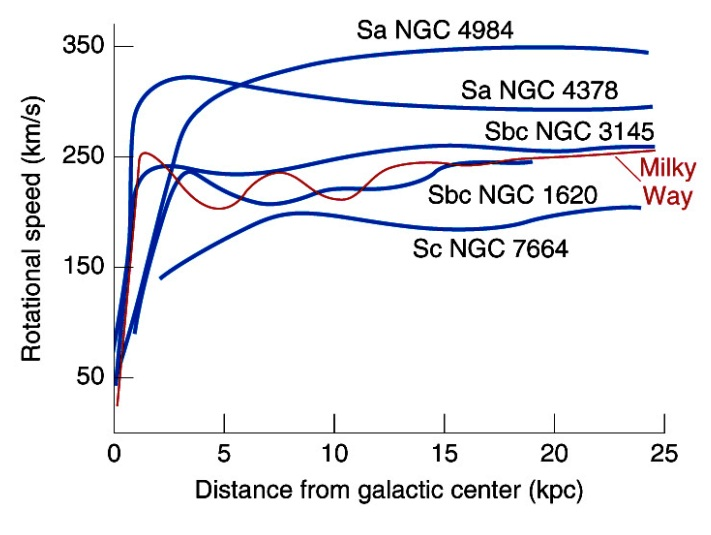
\includegraphics[width=\textwidth]{vcurve.jpg}
\end{center}
\caption{Velocity curves of spiral galaxies. \label{fig:vcurve}}
\end{figure}

Small irregular galaxies can have mass to light ratios of $100$, 
meaning they are even more dark matter dominated than big galaxies.  This is 
thought to be because the shallow gravitational potential of these galaxies 
allows the baryonic matter to be expelled, leaving only the dark matter.  

Candidates for dark matter include massive neutrinos (which we know exist, we 
just don't know how much exists), and theoretical particles like weakly 
interacting massive particles (WIMPS, not to be confused with the glorious 
society) and axions.  Modified Newtonian gravity is another, less popular 
possibility.  In terms of structure formation, dark matter is broken down into 
two classes- hot (HDM) and cold (CDM).  Hot dark matter would be relativistic 
particles such as neutrinos.  The relativistic speeds of HDM would smooth-out 
small-scale density fluctuations in the early Universe, so large structures 
would form first, and smaller structures would form later through fragmentation 
(top-down structure formation).  CDM would consist of slower moving 
particles like WIMPs or axions.  Small density fluctuations would not be 
affected, so small structures would form before large structures (bottom-up 
structure formation).  Most dark matter is probably CDM.  

Dark energy is a complete mystery.  We know the Universe's expansion is 
accelarating due to a cosmological constant $\Lambda$, with 
$\Omega_{\Lambda}\sim0.7$ (see expansion test section).  We don't know what 
dark energy actually is though.  

\subsection{Large Scale Structure}
The Milky Way is part of the local group of galaxies, which is on the edge 
of the much larger local supercluster.  The local supercluster is a $\sim60$ 
Mpc flatten group of galaxies clusters, with the Virgo cluster at its center.  
Other superclusters can be as large as $\sim100$ Mpc.  

Formation of large scale structure:\newline
For structures collapsing on a free-fall timescale, $t_{ff}\propto\rho^{-1/2}$, 
so smaller structures (which tend to be denser) form first.  For example, 
the free-fall time of a galaxy is hundreds of Myr, while for a cluster, the 
timescale is $\sim10$ Gyr.  This means galaxies should have formed early in the 
Universe (at high redshifts), and clusters should still be forming today.  This 
matches what we observe.  If the collapse of material into a cluster is 
non-spherical, the collapse will happen first along the shortest axis, forming 
a pancake.  The next shortest axis will collapse next, forming a thin 
filament.  Finally, it collapses along the remaining axis forming a spherical 
cluster.  We see these pancakes and filaments in numerical simulations and 
observations of large scale structure.  

Observations of large scale structure:\newline
Large scale structure can be mapped in 3-D using redshift surveys.  Mapping 
the positions of galaxies on the sky, then moving through different redshift 
slices reveals that the 3-D distribution of galaxies is not random.  Galaxies 
are in coherent structures.  One problem with using redshifts for this is 
the ``finger of God'' effect.  If a cluster is physically spherical, but has 
velocity dispersion amoung its galaxies, the dispersion velocities of the 
galaxies will add to or subtract from their measured redshifts, causing the 
cluster to appear elongated in redshift space (see Figure \ref{fig:finger}).  
If the cluster is still collapsing, than galaxies on the close side will 
be moving away from us with extra velocity, while galaxies on the far side 
will have extra motion towards us.  This has the effect of flattening 
the galaxy in redshift space.  

\begin{figure}[!h]
\begin{center}
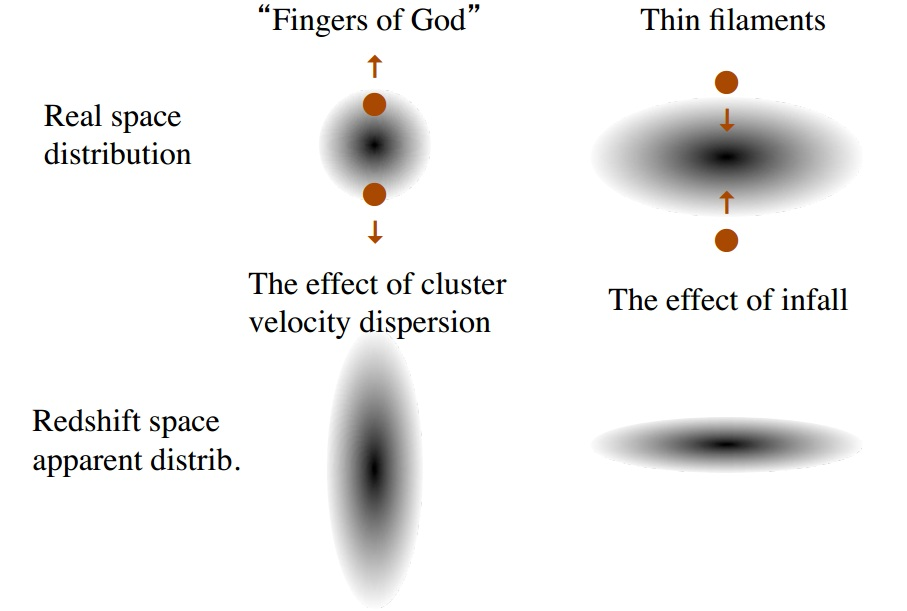
\includegraphics[width=\textwidth]{finger.jpg}
\end{center}
\caption{Velocity dispersion and infall effects on redshift maps. 
\label{fig:finger}}
\end{figure}

2 Point Correlation Function:\newline
The degree to which galaxies are clustered is quantified by the 2 point 
correlation function, $\xi (r)$.  This is defined as the excess 
probability of finding a galaxy a distance $r$ away from another galaxy, 
relative to a uniform galaxy distributin.  In other words, for a uniform 
galaxy distribution, the number of galaxies you'd expect to find a distance 
r away from a single galaxy is $dN(r)=4\pi r^2ndr$ where $n$ is the number 
density of galaxies.  If the galaxies are clustered with a correlation function 
$\xi$, then the number you would find is $dN(r)=4\pi r^2n(1+\xi(r))dr$.  
The 2 point correlation function is usually assumed to be (you guessed it!) a 
power law:
\begin{equation}
\xi(r)=\left(\frac{r}{r_0}\right)^{-\gamma}
\end{equation}
where, for galaxies, $r_0\sim5h^{-1}$ Mpc, and $\gamma\sim1.8$.  For clusters, 
clustering is stronger (clusters of clusters are more clustered than clusters 
of galaxies).  Generally, bigger structures cluster more strongly.  $\xi (r)$ 
can be estimated by counting the number of galaxy pairs in a dataset (DD) 
and by counting the number of pairs in a randomly generated uniform catalog 
(RR).  Then
\begin{equation}
\xi (r)=\frac{DD}{RR}-1
\end{equation}
There are more sophisticated methods to take into account effects at the edges 
of the dataset, but this is the basic idea.  Observations indicate that 
brigher galaxies are more strongly clustered than fainter ones, and redder 
galaxies (ellipticals) are clustered more strongly than bluer galaxies 
(spirals).  To compare with structure formation simulations, a power spectrum 
can be calculated from the Fourier transform of the correlation function.  
The observed power spectrum matches CDM simulations, and shows a peak 
corresponding to the peak in the power spectrum of CMB fluctuations (this 
isn't really explained well on the slide, but I think it has something to do 
with one of the will-ask questions).  

Peculiar Velocities:\newline
Large scale structure can also be probed using the peculiar velocities of 
galaxies.  This is a measure of their motions in addition to their Hubble 
flow velocities, in other words
\begin{equation}
v_{tot}=v_{Hub}+v_{pec}=H_0d+v_{pec}
\end{equation}
This peculiar motion is due to fluctuations in the large scale density field 
(i.e. large scale structure).  The redshifts of galaxies can be measured and 
assumed to be due to only Hubble flow.  The positions of the galaxies this 
gives can be used to find what their accelarations towards each other would 
be.  These accelarations times the Hubble time gives a peculiar velocity 
estimate.  Once the peculiar velocity has been found this way, the positions 
of the galaxies can be updated using only the Hubble contribution to their 
redshifts.  This can be repeated until things converge, giving a final density 
field.  For example, the Milky Way is falling towards the Virgo 
Cluster at $\sim300$ km/s, and the local supercluster is falling towards the 
Hydra-Centaurus Supercluster at $\sim500$ km/s.

Evolution of Clustering:\newline
Large scale structure starts out as primordial density fluctuations that 
continuously collapse under their own gravity.  Therefore, it is expected 
that clustering is stronger today than at high redshifts, since things 
will have collapsed more.  This is what is observed out to $z=1$.  At higher 
redshifts, however, clustering strength increases.  This is because the 
galaxies we see at high redshifts are a biased tracer of clustering.  
For galaxy clusters to have already formed at high redshift, they must 
correspond to higher peaks in the density fluctuations.  We see the light 
from these galaxies and clusters, but not the light from other mass that 
has not yet collapsed.  So all we can see is the few things that are most 
strongly clustered.  For example, 
at high z, the only things that have already started clustering came from 
$5\sigma$ density fluctuations.  These fluctuations collapsed quickly and are 
tightly clustered, so the clustering strenght looks high.  At lower 
redshifts, these $5\sigma$ peaks will be even more strongly clustered, 
but the total clustering strength will be brought down by $1$ and $3\sigma$ 
peaks that have finally had time to form clusters.  So clustering does 
strengthen in time, but today we see a correlation function that is brought 
down by intrinsically less strongly clustered things.  At high z, all we 
can see are intrinsically tightly clustered things.  It's like looking at 
a nearby population of stars and a far away population of stars, and concluding 
the two have different IMFs because all you can see in the distant population 
are massive stars.  

\subsection{Galaxy Clusters}
Galaxy clusters are usuallay a few Mpc across and contain $100-1000$ luminous 
galaxies and many more dwarfs.  Total masses are 
$\sim10^{14}-10^{15}\ M_{\odot}$.  Clusters are gravitationally bound, but 
not all have virialized yet.  Clusters are $\sim80$\% dark matter, $10$\% 
galaxies, and $10$\% hot x-ray gas.  Clusters are denser than galaxy groups 
and are dominated by elliptical galaxies, while groups are dominated by 
spirals.  The closest cluster to us is the Virgo cluster, $\sim3$ Mpc in size, 
$\sim16$ Mpc away, and containing $\sim2000$ galaxies, mostly dwarfs.

Finding Clusters:\newline
Cluster can be identified by finding the galaxies themselves, the x-ray gas, 
or the dark matter.  Using optical observations, overdensities of 
galaxies can be identified.  Also, color information can be used since clusters 
contain many red elliptical galaxies.  The problem with this technique is 
galaxies may appaear close together on the sky, but could be at different 
distances.  Another technique involves using the color-magnitude sequence 
for elliptical galaxies (basically a mass-metallicity relationship).  This 
sequence changes at different redshifts because of the K correction, so 
picking out galaxies along the same sequence can be used to finds ones at the 
same distance.  

The hot IGM gas in clusters can be detected by x-ray observations of thermal 
bremsstrahlung from the gas or by the S-Z effect.  Both of these techniques, 
however, are based on detecting clusters from light, not from mass.  Weak 
lensing can be used to identify the dark matter in clusters, actually detecting 
the clusters based on mass.  This is difficult to do observationally though.  

The Galaxies:\newline
Many (but not all) clusters are dominated by a large elliptical galaxy in the 
center.  The distribution of galaxies can be regular (spherically symmetric 
with increasing density toward the center) or irregular (not spherically, 
with a uniform number density, also contain more spirals).  The interpretation 
is that regular clusters are those that have had time to dynamically relax 
and reach equilibrium.  Mergers have turned the spiral galaxies into elliptical 
galaxies, and built up the large central galaxy.  Irregular clusters 
are still forming and have not come to equilibrium or used up their spirals 
yet.  

The giant elliptical galaxies in the centers of clusters are often surrounded 
by diffuse light from stars that have collected at the center of the cluster.  
These stars (originally noticed by Zwicky) have probably been 
stripped from other galaxies during mergers and have collected in the center 
of the cluster.  This is evidence that the evolution of galaxies is affected 
by their environment.  Another example is the stripping of gas from spiral 
galaxies due to the ram pressure of the IGM x-ray gas.  

The x-ray Gas:\newline
The x-ray gas in galaxy clusters has a typical temperature of $10^7-10^8$ K, 
emitting by thermal bremsstrahlung.  There is too much of this gas for it 
to have all escaped from galaxies, so it must be left over from formation of 
the cluster.  The gas was probably heated by shocks as it fell into the cluster 
potential, and since it can only cool through bremsstrahlung, it is still hot.  
The gas does contain some metals though, so some of it has been added by 
galaxies.  The temperature of the gas can be used in the virial theorem to 
find a cluster mass of $10^{14}-10^{15}\ M_{\odot}$, implying the presence of 
dark matter (see Contents of the Universe section).  The mass profile of the 
cluster can also be found using this gas (I'm not really sure how, the slide 
doesn't give much detail, but this could be used in the galaxies will-ask).  
The x-ray gas is also important for the S-Z effect for finding and determining 
distances to clusters.  As mentioned above, the x-ray gas can strip cold gas 
out of spiral galaxies in the cluster.  As expected, the most gas 
deficient spirals are located in the cores of clusters where the x-ray gas 
density is the highest.  Gas deficiency also correlates with x-ray luminosity 
(which depends on density). 

\subsection{Galaxy Relations}
Hubble Sequence:\newline
Hubble classified galaxies in a tuning fork diagram based on their appearance 
(see Figure \ref{fig:fork}).  Ellipticals are on the left, with the number 
after E corresponding to the ellipticity of the galaxy times $10$, rounded to 
the nearest integer.  The two branches on the right are for spirals with bars 
and spirals without bars.  Left to right on the branches corresponds to 
less tightly wound arms and a less prominent central bulge.  The S$0$ galaxies 
in the center are a cross between ellipticals and spirals.  They have a bulge 
and disk structure, but no spiral arms and a low star formation rate.  Hubble 
originally thought this diagram was an evolutionary sequence, so ellipticals 
are still called early type galaxies and spirals are called late type 
galaxies.  

\begin{figure}[!h]
\begin{center}
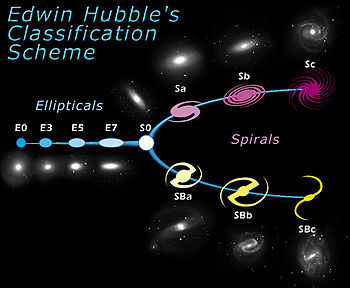
\includegraphics[width=\textwidth]{fork.jpg}
\end{center}
\caption{Hubble Sequence 
\label{fig:fork}}
\end{figure}

Hubble's classification scheme is subjective and based on appearance, not 
physics, but there are still properties that correlate with the sequence.  
Moving from left to right on the diagram, there is a transition from 
pressure support of the galaxy (kinematic pressure) to rotational support, 
an increase in star formation, red color to blue color, hot gas to cold gas 
and dust, old to still forming, and high luminosity density to low luminosity 
density.  These trends represent different star formation histories in 
ellipticals and spirals.  Ellipticals had a large burst of star formation 
early in their histories, using up all of their gas.  So all that's left is 
old, red stars.  Spirals have had a more steady star formation history, and 
are being supplied with new infalling gas (they have star formation rates of a 
few $M_{\odot}$ per year, but only a few $\times 10^9\ M_{\odot}$ of gas).  
Another difference between spirals and ellipticals is formation.  If 
ellipticals formed from the merger of stellar dominated systems, the 
dissipationless collisions would result in a pressure supported system, 
with the stars following the random $3$-D motions that they came in with.  
On the other hand, if clouds of gas merge, energy will be dissapated in the 
process, forming a disk before stars form.  

Scaling Relations:\newline
Properties of galaxies tend to follow power laws, which reflect the actual 
physics of the galaxies (even though we don't understand the physics, like 
Shri says, big galaxies are big).  Such correlations that relate distance 
dependent quantities to distance independent quantities (like the Tully-Fisher 
relation) are useful as distance indicators.  For spiral galaxies, the 
Tully-Fisher relation relates the luminosity and rotational speed of the 
galaxy:
\begin{equation}
L\propto V_{rot}^{\sim4}
\end{equation}
This relation can be hand-wavingly derived by assuming a galaxy disk has 
radius $r_d$ and uniform surface brightness $I$.  Then the total luminosity 
of the galaxy is given by $L\propto r_d^2I$.  Using the virial theorem, the 
mass inside of $r_d$ is $M\propto r_dV_{rot}^2$.  These two equations can 
be combined to give:
\begin{equation}
L\propto \left(\frac{M}{L}\right)^{-2}V_{rot}^4I^{-1}
\end{equation}
If if is assumed that all spirals have the same mass to light ratio and 
surface brighteness, then this becomes 
\begin{equation}
L\propto V_{rot}^4
\end{equation}
The surprising thing about the Tully-Fisher relation is it connects a property 
of the dark halo ($V_{rot}$) to a property of the visible matter ($L$), so 
there must some sort of feedback mechanism relating the two.  Elliptical 
galaxies follow the same proportionallity between their luminosity and 
velocity dispersion, known as the Faber-Jackson relation:
\begin{equation}
L\propto \sigma^4
\end{equation}

Fundamental Plane:\newline
Observationally, elliptical galaxies line in a plane in radius, surface 
brightness, velocity dispersion space defined by 
\begin{equation}
R\propto \sigma^{1.4}I^{-0.8}
\end{equation}
Sometimes luminosity is used instead of radius:
\begin{equation}
L\propto \sigma^{3.26}I^{-0.8}
\end{equation}
This can be approximately derived starting with the Virial Theorem
\begin{equation}
\frac{GM}{<R>}=k_E\frac{<V^2>}{2}
\end{equation}
and assuming that the observable radius, velocity dispersion, and luminosity 
(without the brackets) are related to the actual average $3$-D values (with 
the brackets) by $R=k_R<R>$, $V^2=k_V<V^2>$, and $L=k_LIR^2$.  I think all of 
these k's are just accounting for the fact that this is handwavy and 
approximate.  Solving for 
mass in the Virial Theorem and dividing by luminosity and rearranging gives:
\begin{equation}
R=K_{SR}V^2I^{-1}(M/L)^{-1}
\end{equation}
\begin{equation}
L=K_{SL}V^4I^{-1}(M/L)^{-2}
\end{equation}
with 
\begin{equation}
K_{SR}=\frac{k_E}{2Gk_Rk_Lk_V}
\end{equation}
\begin{equation}
K_{SL}=\frac{k_E^2}{4G^2k_R^2k_L^2k_V^2}
\end{equation}
The relations for $R$ and $L$ are a little off from the observed relations, 
meaning either the k's or the mass to light ratio varies with the fundamental 
plane parameters.  If lensing is used to to replace surface brightness with 
surface density, observations give 
\begin{equation}
R\propto \sigma^{1.8\pm0.2}\Sigma^{-1\pm0.2}
\end{equation}
consistent with the Virial Theorem derivation.  Looking at the fundamental 
plane with different pairs of parameters gives other relations, such as the 
Faber-Jackson relation and the Kormendy relation:
\begin{equation}
R\propto I^{-0.8}
\end{equation}
Scatter in these relations is just scatter due to the other axis of the $3$-D 
space.  

The fundamental plane is surpising because if means elliptical galaxies 
only occupy a small part of their possible parameter space, regardless of 
their formation or evolution histories.  Simulations can reproduce the plain, 
but not explain it.  

Other correlations George mentioned are the correlation between black hole 
mass and K-band absolute magnitude ($M_{BH}\propto M_K$) and the correlation 
between black hole mass and velocity dispersion ($M_{BH}\propto \sigma^{4.5}$) 
for spiral bulges and ellipticals.  These relations are not fully understood, 
but probably have to do with some sort of feedback.  

Dwarf Galaxies:\newline
Dwarf ellipticals and dwarf spheroidals are classified with regular ellipticals 
in the Hubble sequence, but follow different scaling relations.  For example, 
while regular ellipticals show decreasing average surface brightness with 
increasing total luminosity, while dwarfs follow an opposite trend.  The 
difference is the different formation and evolutionary processes for dwarf 
galaxies.  With less mass, these galaxies are less able to hold onto their gas, 
so the first generation of supernovae can blow the gas out of the galaxy, 
leaving the galaxy with a few stars and lots of dark matter.  



\section{High Energy}
\subsection{Questions}
\begin{enumerate}
\item \textbf{Describe the mechanisms by which cosmic rays gain and lose energy. Which mechanisms
      are appropriate to which type of particle? Which ones produce electromagnetic
      radiation that we can observe, and in what wave bands?}

      \begin{figure}[ht]
      \centering
      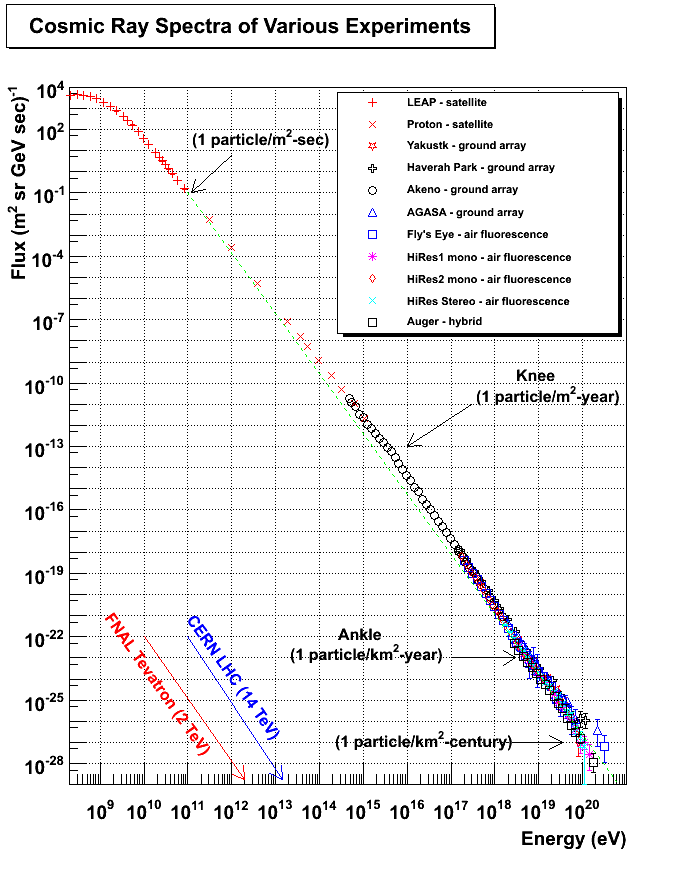
\includegraphics[width=\textwidth]{highenergy_cosmic_ray_spectrum}
      \caption{The ``specific intensity'' of cosmic rays as a function of energy.  Although this
               is almost a perfect power law over 11 orders of magnitude (!), there are two
               important features: the knee at $10^{15}~{\rm eV}$ and the ankle at $10^{18}~{\rm eV}$.}
      \label{fig:cosmic_ray_spectrum}
      \end{figure}

      \newthought{Let's begin by} discussing a few properties of cosmic rays.  At the top of
      the atmosphere, 98\% of cosmic rays are protons and nuclei, while 2\% are electrons.
      Of the protons and nuclei, 87\% are protons, 12\% are helium nuclei, and the remaining
      1\% are more massive nuclei.
      See Figure~\ref{fig:cosmic_ray_spectrum} for the differential energy spectrum at the top of the
      atmosphere (interactions with the atmosphere can produce secondary cosmic rays).
      For protons and nuclei we have
      \begin{dmath}
        N(E)\,\d E \approx 1.8\times10^4\,\left(\frac{E}{\rm GeV}\right)^{-2.7}
                           \,\d E\,{\rm nucleons}\,{\rm m}^{-2}\,{\rm s}^{-1}\,{\rm sr}^{-1}
      \end{dmath},
      while for electrons we have
      \begin{dmath}
        N(E)\,\d E \approx 700\,\left(\frac{E}{\rm GeV}\right)^{-3.3}
                           \,\d E\,{\rm nucleons}\,{\rm m}^{-2}\,{\rm s}^{-1}\,{\rm sr}^{-1}
      \end{dmath}.
      The steeper power law for electrons reflects the fact that electrons are less massive
      and hence lose energy more easily.

      \begin{figure}[ht]
      \centering
      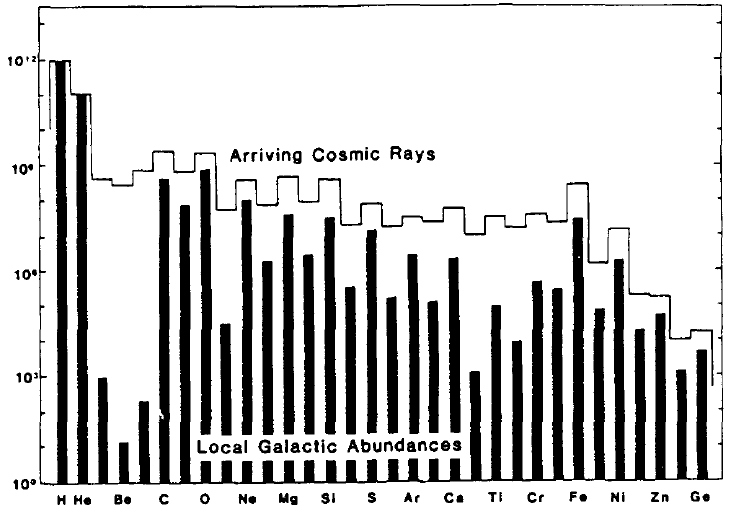
\includegraphics[width=\textwidth]{highenergy_cosmic_ray_abundances}
      \caption{The elemental abundances seen in cosmic rays compared with the local galaxy.
               Note the overabundances of lithium, beryllium, and boron.  A similar
               overabundance is seen near titanium.  The pattern of even elements being more
               common than odd elements (due to the alpha capture process in stars) is seen to
               a lesser extent.  The abundance of heavy elements is remarkably flat.}
      \label{fig:cosmic_ray_abundances}
      \end{figure}

\item \textbf{Discuss the equation of state of relativistic/nonrelativistic degenerate gases of electrons
      and neutrons and derive the Chandrasekhar mass limit for white dwarfs. (A
      heuristic approach, as in Shapiro and Teukolsky, is sufficient.)}
      
      \newthought{Let's derive the} degeneracy pressure for non-relativistic electrons. First we look at
      the Heisenberg uncertainty principle, which states that
      $\Delta x \Delta p \ge \frac{\hbar}{2}$.  This suggests that there's a minimum volume
      of phase space that can be occupied by two electrons\sidenote{
        The factor of two comes from the fact that electrons of opposite spin can occupy
        the same region of phase space.
      }.  By definition of the Planck constant, this minimum volume is
      \begin{dmath}
        \Delta x\,\Delta y\,\Delta z\,\Delta p_x\,\Delta p_y\,\Delta p_z = h^3
      \end{dmath}.
      The phase-space density $n(p)\,\d p = (2/h^3)\,4\pi p^2\,\d p$, since two electrons
      can occupy each cell of volume $h^3$.

      To get the spatial electron density, integrate over momentum to find
      \begin{dmath}
      n_e = \int_0^{p_F} n(p)\,\d p \nolinebreak = \frac{8 \pi}{3 h^3}p_F^3
      \end{dmath},
      where we have assumed that $T=0$ (or rather that thermal pressure is very small compared to
      degeneracy pressure), so the maximum momentum is the Fermi momentum. We now know that
      \begin{dgroup}
      \begin{dmath}
      p_F = \left( \frac{3 h^3}{8 \pi} n_e \right) ^{1/3} \nolinebreak
          = \left( 3 \pi^2 n_e \right) ^{1/3}\hbar
      \end{dmath}
      \begin{dmath}
      E_{F,{\rm non-relativistic}} = \frac{p_F^2}{2m_e} \nolinebreak
                                   = \frac{1}{2m_e}\left( \frac{3 h^3}{8 \pi} n_e \right) ^{2/3}
      \end{dmath}
      \begin{dmath}
      E_{F,{\rm relativistic}} = p_Fc \nolinebreak
                               = \left( 3 \pi^2 n_e \right) ^{1/3}\hbar c
      \end{dmath}
      \end{dgroup}
      
      %Now let's figure out how to get the pressure. %Define the phase space distribution $\tilde{f} = \frac{g_s}{h^3} f$, where $g_s = 2S + 1$ which is $2$ in the case of spin-1/2 particles. The pressure is defined by
      Now let's find the pressure.  Begin with the pressure integral
      \begin{dmath}\label{eq:pressure_integral}
      P = \frac{1}{3} \int p v n(p)\,4 \pi p^2\,\d p
      \end{dmath}.
      We also know the electron density
      \begin{dmath}
      n_e = \frac{\rho}{\mu_e m_H},~\mu_e \nolinebreak = \frac{A}{Z} \nolinebreak \approx 2
      \end{dmath}
      for a regular white dwarf.
      
      In the non-relativistic case $v = p/m_e$. Then integrating Equation~\ref{eq:pressure_integral}
      gives us
      \begin{dmath*}
      P_{\rm non-relativistic} = \frac{8\pi}{3h^3m_e}\int^{p_F}_0 p^4\,\d p \nolinebreak
                               = \frac{8\pi}{15h^3m_e}p_F^5
      \end{dmath*}.
      Plugging in for $p_F$ gives
      \begin{dmath}\boxed{
      P_{\rm non-relativistic} = \frac{h^2}{20m_e}\left(\frac{3}{\pi}\right)^{2/3}\left(\frac{\rho}{\mu_em_H}\right)^{5/3}
      }\end{dmath}
      Notice that $P\propto\rho^{5/3}$, so we have a polytropic equation of state.\sidenote{
        It's also convenient to write this as
        $P_e = k_1^\prime \biggl( \frac{\rho}{\mu_e} \biggr)^{5/3}$ so the degeneracy pressure
        depends on both the density and the electron fraction of the gas. If there are nuclear
        reactions going on, $\mu_e$ may change and $k_1$ will not be constant.
      }
      
      Now let's look at the very relativistic case. Here we can approximate $v \sim c$, and the pressure becomes
      \begin{dmath*}
      P_{\rm relativistic} = \frac{8\pi c}{3h^3}\int^{p_F}_0 p^3\,\d p \nolinebreak
                           = \frac{2\pi c}{3h^3}p_F^4
      \end{dmath*}.
      This can be rewritten as
      Plugging in for $p_F$ gives
      \begin{dmath}\boxed{
      P_{\rm relativistic} = \frac{hc}{8}\left(\frac{3}{\pi}\right)^{1/3}\left(\frac{\rho}{\mu_em_H}\right)^{4/3}
      }\end{dmath}
      This we can rewrite as $P_{e,r} = k_2 \rho^{4/3} = k_2^\prime \biggl(\frac{\rho}{\mu_e}\biggr)^{4/3}$, so this is also a polytrope but with adiabatic index $4/3$. We will see in a second that this is key to showing that white dwarfs have a maximum mass once their electrons become ultrarelativistic.
      
      \newthought{Here's one derivation} of the Chandrasekhar mass limit.
      Use the relativistic electron degeneracy pressure and hydrostatic equilibrium, which we will wave into this form:
      \begin{equation}
      \frac{P}{R} \sim \frac{G M \rho}{R^2} \sim \frac{3 G M^2}{4 \pi R^5}\,\,.
      \end{equation}
      Set this equal to our adiabatic pressure to get
      \begin{equation}
      P \approx \frac{3 G M^2}{4 \pi R^4} \sim k_2 \rho^{4/3} \approx k_2 \biggl(\frac{3 M}{4 \pi R^3}\biggr)^{4/3}\,\,.
      \end{equation}
      Rearranging, we get
      \begin{equation}
      M^{2/3} \approx \biggl(\frac{4\pi}{3 G} \biggr)\biggl(\frac{2\pi c}{2 h^3} \biggr)\biggl(\frac{3 h^3}{8 \pi \mu_e m_H} \biggr)^{4/3} \biggl(\frac{3}{4 \pi} \biggr)^{4/3}
      \end{equation}
      Note that this formula for the mass is all constants (assuming $\mu_e$ doesn't change)! That means mass no longer scales with radius or anything else, and we have found a unique mass at which electrons must travel at the speed of light in order to support it. The numbers work out to give $5.6 \times 10^{32}~{\rm g}$. This is off by a factor of 5 from the value we want.

      \newthought{Alternatively, we can use} energy considerations to find the Chandrasekhar mass.
      Begin by writing the total energy\sidenote{
        Note that thermal energy is unimportant compared to the Fermi energy here.
      } as
      \begin{dmath}
        E = E_{\rm F}N_e - q\frac{GM^2}{R}
      \end{dmath},
      where $N_e$ is the total number of electrons and $q$ is a constant factor of order unity.
      The total number of electrons is $M/\mu_e m_H$, and the Fermi energy (in the
      ultra-relativistic case is)
      \begin{dmath*}
      E_{F,{\rm relativistic}} = \left( 3 \pi^2 n_e \right) ^{1/3}\hbar c
                               = \left(3\pi^2\frac{3N_e}{4\pi R^3}\right)^{1/3}\hbar c
                               = \left(\frac{9\pi}{4}\frac{M}{\mu_e m_H}\right)^{1/3}\frac{\hbar c}{R}
      \end{dmath*}.
      Notice that the Fermi and gravitational contributions to the total energy both scalse $\propto R^{-1}$.
      Hydrostatic equilibrium occurs at a local minimum of $E$, but this can only be satisfied
      (in this case) when $E=0$.  Therefore
      \begin{dgroup*}
      \begin{dmath*}
        q\frac{GM^2}{R} = E_{\rm F}N_e
      \end{dmath*}
      \begin{dmath*}
        q\frac{GM^2}{R} = 
        \left(\frac{9\pi}{4}\right)^{1/3}\left(\frac{M}{\mu_em_H}\right)^{4/3}\frac{\hbar c}{R}
      \end{dmath*}
      \begin{dmath}\boxed{
        M = \left(\frac{9\pi}{4}\right)^{1/2}\left(\frac{1}{\mu_em_H}\right)^{2}\left(\frac{\hbar c}{qG}\right)^{3/2}
      }\end{dmath}.
      \end{dgroup*}
      Taking $q\sim 1$ (note that $q<1$ in all physical cases), we find $M\approx1.2M_\astrosun$
      for the Chandrasekhar mass limit.

      \newthought{I just had a} brilliant idea!  Let's use the Buckingham $\Pi$ theorem to
      derive the Chandrasekhar mass.  Quantum mechanics is important here, so we'll include
      $\hbar$.  The speed of light is also important because we need relativistic degeneracy
      pressure.  Gravity is important, so include $G$.  Finally, the mass per electron is
      important, so we'll include the mass of hydrogen.

      \begin{table}[ht]
      \centering
      \begin{tabular}{cc}
      \toprule
      Constant & Units \\
      \midrule
      $\hbar$ & $ML^2T^{-1}$ \\
      $c$ & $LT^{-1}$ \\
      $G$ & $M^{-1}L^3T^{-2}$ \\
      $m_H$ & $M$ \\
      $M_{\rm Chandrasekhar}$ & $M$ \\
      \bottomrule
      \end{tabular}
      \caption{The constants that are relevant for defining the Chandrasekhar mass.}
      \label{tab:chandrasekhar_mass_constants}
      \end{table}

      Now the Chandrasekhar mass arises because we're trying to squeeze too many electrons into
      a small volume.  In order for electrons to occupy the same physical location, they must
      have different velocities.  However, eventually you run into the speed of light.
      Therefore the higher the speed of light is, the higher the Chandrasekhar mass should be.
      Similarly, if gravity is stronger, the Chandrasekhar mass should be lower.

      Looking at Table~\ref{tab:chandrasekhar_mass_constants} we have 5 constants and 3 units,
      so there are 2 dimensionless $\Pi$s.  These are
      \begin{dgroup}
      \begin{dmath}
        \Pi_1 = \frac{M_{\rm Chandrasekhar}}{m_H}
      \end{dmath}
      \begin{dmath}
        \Pi_2 = \frac{\hbar c}{m_H^2G}
      \end{dmath}.
      \end{dgroup}
      Now in general we can write
      \begin{dgroup*}
      \begin{dmath*}
        \Pi_1 = f(\Pi_2)
      \end{dmath*}
      \begin{dmath*}
        M_{\rm Chandrasekhar} = m_H\,f\left(\frac{\hbar c}{m_H^2G}\right)
      \end{dmath*}
      \end{dgroup*}
      Now we simply need to show from a brief physical analysis how $M_{\rm Chandrasekhar}$
      should depend on one of these constants (see the previous derivations, but you can
      discard all the other constants).  This gets you
      \begin{dmath}\boxed{
        M_{\rm Chandrasekhar} = \frac{1}{m_H^2}\left(\frac{\hbar c}{G}\right)^{3/2} \nolinebreak
                              = 1.85\,M_\astrosun
      }\end{dmath}.
      
\item \textbf{Derive the equation for the effective temperature of an accretion disk around a
      black hole of mass $M$ with accretion rate $\dot M$, as a function of radius $r$. Specify the
      assumptions required to get an answer, and comment on what could go wrong with
      them. Define the Eddington luminosity and explain its relevance to the peak frequency
      of the emitted radiation.}
      
      Consider the vertical structure of an accretion disk, assume we're at large radii ($r \gg r_{\rm in}$), and assume it's a thin disk radiating mostly just through the top and bottom. The heating rate per volume is
      \begin{equation}
      \nabla \cdot F_{\rm rad} = \rho \nu (r \Omega^\prime)^2 = \rho \nu \biggl(\frac{3}{2} \Omega \biggr)^2
      \end{equation}
      from assuming that the rotation is Keplerian. Use radiative diffusion with $P_{\rm rad} = \frac{1}{3} a T^4 = \frac{1}{3}\frac{4 \sigma_{\rm SB}}{c}T^4$. Assume that the disk is optically thick enough that the spectrum is a blackbody. Assume radiation travelling through a layer that is one mean free path $\lambda = 1/\kappa \rho$ thick is what's giving you the flux. The flux is then the speed of light times the mean free path times the change in radiation pressure with height (note: I have not totally justified this expression. If anyone can shed light on this, that'll be cool):
      \begin{equation}
      F_{\rm rad} - \frac{1}{\kappa \rho} \frac{d}{dz}P_{\rm rad} c = -\frac{4}{3}\frac{\sigma_{\rm SB}}{\kappa \rho}\frac{\partial T^4}{\partial z}
      \end{equation}
      This is similar to the radiative diffusion equation for stars\footnote{$L(r) = -4 \pi r^2 \frac{4}{3} \frac{c a T^3}{\kappa\rho}\frac{\partial T}{\partial r}$}. Now let's integrate vertically, because we want the total flux from each vertical layer in the accretion disk coming out of the top and bottom of the disk.
      \begin{equation}
      \int^\infty_0 \frac{\partial F_{\rm rad}}{\partial z} = \sigma T_{\rm eff}^4 = \frac{1}{2} \Sigma \langle \nu \rangle \frac{9}{4}\Omega^2 = \frac{9}{8} \frac{G M \dot{M}}{3 \pi r^3}
      \end{equation}
      Now approximate 
      \begin{equation}
      -\frac{4}{3} \frac{\sigma_{\rm SB}}{\kappa rho} \frac{\partial T^4}{\partial z} \approx D(r) = \frac{3}{8 \pi}\frac{GM\dot{M}}{r^3}\biggl[1 - \sqrt{\frac{r_{\rm in}}{r}} \biggr]
      \end{equation}
      
      We eventually want to get here:
      \begin{equation}
      D(r) \approx \frac{4}{3}\frac{\sigma_{\rm SB}}{\kappa \rho}\frac{T^4_{\rm midplane}}{H} \approx \frac{4}{3}\sigma_{\rm SB}\frac{T^4_{\rm midplane}}{\tau_{\rm vert}} = \frac{4}{3}\sigma_{\rm SB}T^4_{\rm eff}
      \end{equation}
      
      
\end{enumerate}

\subsection{Fluids and the Sonic Point}

For reference, here is the general equation for accretion and winds for which you have a steady state, that is, $\dot{M} = 4 \pi r^2 \rho v$ is a constant with radius:

\begin{equation}
\frac{1}{v} \frac{dv}{dr} (v^2 - c_s^2) = \frac{2 c_s^2}{r} - \frac{G M}{r^2}\,\,.
\end{equation}
Solutions are depicted in Figure \ref{f:mach}. The point where $v = c_s$ is called the sonic point, and it represents the transition between subsonic and supersonic flow.

\subsection{Star Cores}

\begin{figure}[!h]
\begin{center}
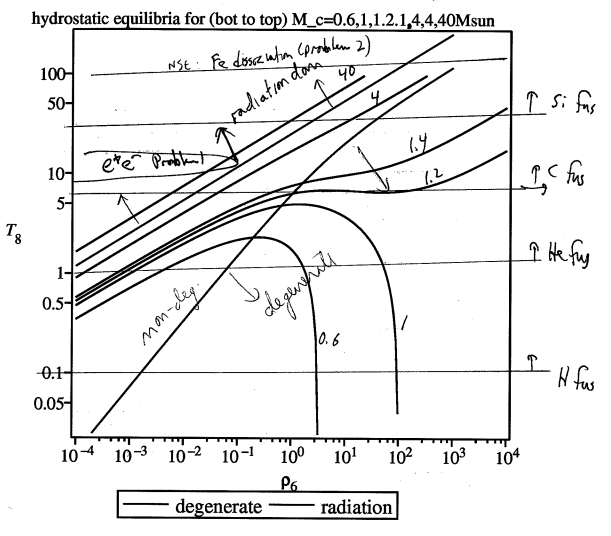
\includegraphics[width=\textwidth]{HE_starcore.jpg}
\caption{Temperature/density tracks of stars with various core masses. This plot is separated into degenerate and nondegenerate regions, and the temperatures at which fusion of various elements start are shown. \label{f:starcore}}
\end{center}
\end{figure}

\subsection{White Dwarfs}

\subsection{Supernovae}

Let's start with core-collapse supernovae. This occurs for stars with a ZAMS mass of $\sim 8-10$ solar masses or higher (the actual cutoff is debateable). These stars have burned through H, He, C, O, Ne, Si, all the way up to iron. At the beginning of every core burning phase, the core has contracted until the temperature was high enough to start fusing the next main isotope in the series. However, iron is the element with the most binding energy per nucleon. See Figure \ref{f:be} for the binding energy curve, showing $^{56}Fe$ at the top. This is therefore the most energetically favorable isotope.

\begin{figure}[!h]
\begin{center}
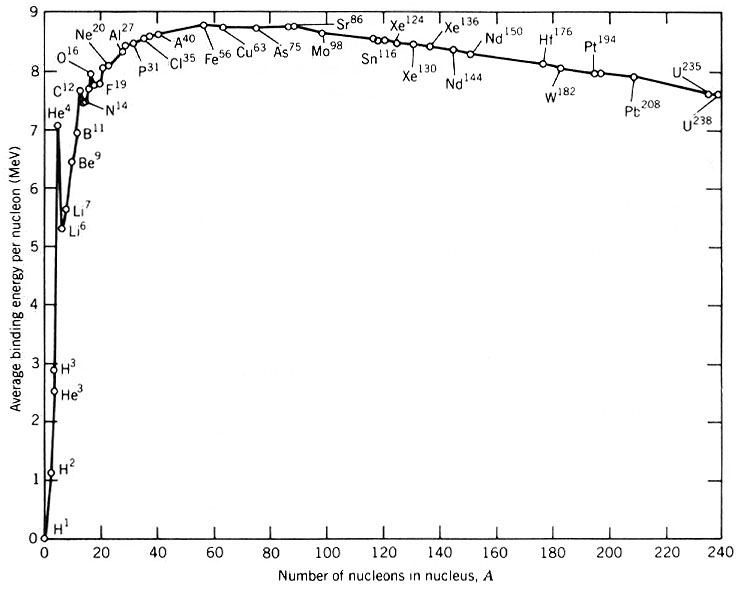
\includegraphics[width=\textwidth]{binding_energy.jpg}
\caption{Binding energy per nucleon. The peak is Fe-56, which is the most stable isotope. \label{f:be}}
\end{center}
\end{figure}

So, what happens when you get a massive iron core? At this stage, the electrons are fully degenerate, but it's good to note that not all the pressure comes from degeneracy, since the core temperature is still quite high (probably close to $10^{10}-10^{11}~{\rm K}$. The core starts to contract, as it did at the end of every other burning phase. As a result, the temperature increases, but this time, there is no other isotope we can fuse iron into and extract energy to re-expand the core. Instead, the temperature continues to increase until photons are energetic enough to start photodissociating iron nuclei into alpha particles and neutrons and photodissociating alpha particles into neutrons and protons. This robs the core of some of its pressure support, which is a combination of thermal and photon pressure, because a bunch of photon energy goes into breaking these nuclei apart. Note that this effect is more important in more massive stars, which have higher core temperatures. Meanwhile, neutronization has been happening at the same time. This starts occurring during Si burning, but when the Fe core grows very massive, it can produce a runaway that saps the core of its electron degeneracy pressure. The neutronization (which is through inverse beta decay), removes electrons and therefore reduced the electron degeneracy pressure. This is what eventually causes the core to collapse rapidly to a neutron star. This also ``deleptonizes" the core by sending out neutrinos, which don't interact much with matter and escape rapidly at this state. The timescale for this collapse is roughly the freefall timescale
\begin{equation}
\tau_{ff} \approx (G\rho)^{-1/2} \approx \biggl(\frac{GM}{R^3}\biggr)^{-1/2} \approx \biggl(\frac{G{\rm M}_\odot}{(6\times 10^8~{\rm cm})^3}\biggr)^{-1/2} \approx 1.2~{\rm s}\,\,.
\end{equation}
Some people quote the freefall time as 0.1-0.5 s, so this gets it to an order of magnitude.

Anyway, now we've rapidly collapsed our entire Chandrasekhar-mass iron core into a neutron star. What happens to everything else? Well, this collapse is much faster than the sound-crossing time of the star. It takes the outer layers a lot more time to ``learn" about the sudden loss of support from below. Note that the core radius is tiny, something like an Earth radius, while the rest of the star may be several to a thousand solar radii. There is not a super sharp cutoff for which layers follow the core and which hang for a bit, but they are basically divided into these two groups. The outer layers of the star then start falling supersonically (I think) toward the core. Meanwhile, the core density roughly equals and surpasses the nuclear density, which is something like $10^{14}~{\rm g}~{\rm cm}^{-3}$. Through rapid collapse, it's overshot its equilibrium as the nuclear strong force takes over pressure support. This causes the core to ``bounce" and the surface moves out a bit very rapidly, right into the falling outer layers. This creates a powerful shock that then propagates outward into the still infalling layers of the star. Much of the shock energy goes into thermally heating the layers of the star and dissociating heavy elements as well as causing explosive nucleosynthesis. This is dominated by the production of $^{56}Ni$ because the layers outside the core are mostly symmetric ions, meaning they have the same numbers of protons and neutrons. Nickel is the most energetically favorable nucleus under the conditions of this rapid nucleosynthesis of symmetric matter, whereas iron was most favorable when there were more neutrons than protons.

The shock has lost a lot of its energy now, even before it reaches the surface. Depending on the energy in the shock, the density of the material, and the radius of the star (i.e. how much matter the shock needs to get through), it will most likely stall. This may not be the case for low-density matter and small radii, but for Type II supernovae (big hydrogen layer) it's very likely. Through some mechanism, we need to revive the shock if we want an explosion.

Meanwhile, the neutron star is super hot and is cooling by releasing neutrinos. These come from the inverse beta decay processes that have been happening before and during collapse:
\begin{equation}
e^- + p \rightarrow \nu_e + n\,\,.
\end{equation}
In fact, this is where most of the energy from the core collapse goes. If we calculate the difference between the gravitational binding energy of the pre-collapse core and the resulting proto-NS, it's about $10^{53}$ ergs! Spoiler alert---that's 100 times as much as the energy we actually see coming out of a supernova based on its line velocities and luminosity. It seems like the best way to reconcile all this is to somehow get 1\% of the energy from neutrinos deposited into the outer layers of the collapsing star in order to revive the shock and get an explosion as we observe. It's not a crazy idea, since the densities become so high that neutrino interactions should be important but we still haven't really pinned this down. There are a couple other possible explanations for how to revive the shock, such as through fluid instabilities, but neutrinos seem like the most viable way right now. Eventually the supernova enters a phase of homologous expansion, which for a fluid element is described by $r = v t$. Everything is expanding at a constant rate, and things that are moving away from the explosion site faster are farther from it proportionally. This holds until the ISM gets in the way (see the ISM section for later phases of supernova remnant expansion).

Okay, we've successfully blown up our star. What do we expect to see? The first thing should be what's called ``shock breakout". This is just when the shock reaches the surface of the star, and there should be a burst of high-energy radiation associated with that. So far it hasn't been observed because it occurs on a very short timescale (I would say minutes to hours), and we'd have to be pointing directly at the supernova while this happens. Then it goes dark---a lot of energy has just been deposited into the outer layers of the star, but it's so dense that the photons haven't had time to diffuse out yet. When they do, there is a gradual rise to roughly peak brightness over the course of a few days to a week.

This is where supernovae from stripped-envelope stars (SNe Ib, Ic) differ from stars that mostly still have their big fat layer of hydrogen (SNe II). For stars without this envelope, energy deposited directly from the shock is not that significant for powering the supernova light curve. Instead it is mostly the decay of $^{56}{\rm Ni}$ to $^{56}{\rm Co}$ (half life $\sim 6$ days to $^{56}{\rm Fe}$ (half life $\sim 80$ days) that supplies all the power. These are beta decays accompanied by gamma-ray emission in the center of the explosion near the proto-NS, and these gamma-rays are thermalized in the ejecta and the energy is re-emitted partly at optical wavelengths, which is why we see this energy come out in the optical. The relationship between the observed peak of the supernova and the is given by Arnett's law, which assumes that the luminosity at peak is given roughly by the total amount of nickel produced (I should find a good expression of Arnett's law and put it here). Anyway, at first the ejecta expands adiabatically and we don't see much because all these photons are trapped inside. The diffusion time is
\begin{equation}
t_{\rm diff} = \frac{N\lambda}{c} \sim \frac{R^2}{\lambda c} \sim \frac{R^2}{c} \kappa \rho
\end{equation}
Once the photon diffusion time roughly equals the time since explosion, all these photons start to escape, and then the light curve dips to follow the cobalt decay tail (see Figure \ref{f:sn_lc}. This diffusion takes about 20 days.

For Type II supernovae, the story is a bit different. Here the ejecta are dominated by a thick hydrogen layer (of course, there will be some situations in between these and Ib types, so you could have sort of hybrid cases). The shock-heated ejecta expand adiabatically as before, and radioactive decays are still depositing photons into the ejecta, which we can't see yet. Then the luminosity goes up as the ejecta expands---however, the luminosity is mediated not immediately by radioactivity but by hydrogen recombination.

\begin{figure}[!h]
\begin{center}
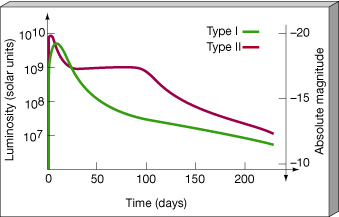
\includegraphics[width=\textwidth]{sn_lc.jpg}
\caption{Approximate light curves for Type I and Type II supernovae. \label{f:sn_lc}}
\end{center}
\end{figure}

Hydrogen recombines at roughly a single temperature $\sim 10^4~{\rm K}$. As we look at the ejecta, it starts out ionized, but the temperature in the outer layers drops to the recombination temperature, and the opacity drops dramatically. In the optical, at least, we basically see down to where the hydrogen is recombining. This front moves inward in comoving (or mass) coordinates, as more of the inner layers cool---but the layers are also moving outward in real space coordinates. The net effect is that the radius at which most of your light is being emitted stays roughly the same. The temperature also stays roughly the same, so this results in a ``plateau" in luminosity for about 100 days. After we've seen through the entire hydrogen layer, which has become optically thin, the light curve proceeds in a way similar to Type I supernovae, following a cobalt decay tail (again see Figure \ref{f:sn_lc}.

Now let's talk about thermonuclear supernovae, the most common of which are Type Ia supernovae. These come generally from C/O-dominated white dwarfs that are close to the Chandrasekhar mass. Contrary to popular belief, they don't generally blow up quite at the Chandrasekhar mass. This is just the maximum mass a white dwarf can have before relativistic electron degeneracy pressure can no longer support it. What actually matters is when you're allowed to unstably burn carbon. 

The general picture people have on how to get a white dwarf under such conditions encompasses two possibilities: single-degenerate (white dwarf accretes from a normal star that has overflowed its Roche lobe, probably depositing hydrogen) and double-degenerate (two white dwarfs merge or collide). There is some debate about which is more likely or whether you can have one or the other, but it's probably one of these two situations. The important thing is that you get your white dwarf up to a certain mass, meaning you get certain temperatures and densities in the center. Once the temperatures and densities are high enough, carbon burning starts (and to some extent oxygen), and this fuels some confection and a deflagration flame. The physics isn't very well known at this point, and there are a few different theories I won't go into about how this actually ends up disrupting the star. But basically you end up with a runaway reaction in which carbon is burning and raising the temperature, which doesn't actually change the pressure support in the star because the pressure is dominantly from degenerate electrons. This causes a runaway, pretty analogous to the helium flash, and at some point this runaway carbon burning turns from a subsonic deflagration into a supersonic detonation, but we currently aren't that clear on how this happens.

This burning of carbon and oxygen to heavier elements ends up being enough to unbind the star, obliterating it completely (whereas in core-collapse supernovae there is a remnant left behind). Sort of surprisingly, it turns out that the total energy is similar to that released in core-collapse supernovae (not in neutrinos), about $10^{51}~{\rm ergs}$. The luminosity is somewhat more than for core-collapse supernovae, $\sim10^{43}~{\rm ergs}~{\rm s}^{`-1}$ rather than $\sim10^{42}~{\rm ergs}~{\rm s}^{`-1}$, so these are the most commonly observed supernovae even though core collapse are actually more common.

These supernovae are, like other Type I supernovae, powered predominantly by radioactive decay, and so their light curves look very similar to those of SNe Ibc, although generally brighter and over a longer timescale (i.e. more nickel is formed in these explosions).

One thing we don't know is what happens if a white dwarf gets dense enough in its center for electron capture to happen ($\sim 4\times 10^4~{\rm g}~{\rm cm}^{-3}$) before you can start runaway carbon burning. This is more likely for O/Ne/Mg white dwarfs, since electron capture onto Mg and Ne is easier than onto C and O (and C is what you need to burn unstably). These should come from intermediate ZAMS mass stars, $6-8$ or $8-10$ solar masses, depending on whom you ask. In this case, the white dwarf could theoretically collapse to a neutron star and create a really weak explosion, which is the topic of io's research. :) These, like Type Ia supernovae, can occur theoretically by either the single-degenerate or double-degenerate channel.

\textbf{Good numbers to know} about normal supernovae of any type: $E \sim 10^{51}~{\rm ergs}$, $M_{\rm ej} \sim 1~{\rm M}_\odot$, $L \sim 10^{42-43}~{\rm ergs}~{\rm s}^{`-1}$, $v_{\rm ej} \sim 10,000~{\rm km}~{\rm s}^{-1}$.

\subsection{Neutron Stars}

A lot of the neutron stars we see are pulsars.

\subsection{Black Holes}

The first thing to know about black holes is that their escape velocities are greater than the speed of light. The hand-wavey way to derive the Schwarzschild radius is to set the gravitational potential energy $\frac{-G Mm}{r}$ equal to the kinetic energy of a classical particle orbiting it $\frac{1}{2}m v^2$, then setting the orbital velocity equal to the speed of light. This gives the result
\begin{equation}
R_s = \sqrt{\frac{2GM}{c^2}}\,\,.
\end{equation}
Of course, the real way to derive this radius is using general relativity, but I think this approach will suffice. Note: if you try to derive this by setting the gravitational force equal to the centripetal force experienced by the particle, you will be off by a factor of two.

The mean density of a black hole is given approximately by finding $\frac{M}{R_s^3}$, which is roughly
\begin{equation}
\frac{M}{\biggl( \frac{GM}{c^2} \biggr)} \approx 6 \times 10^{17} \biggl(\frac{M}{{\rm M}_\odot} \biggr)^2~{\rm g}~{\rm cm}^{-3}\,\,.
\end{equation}
This density is important for determining how important tidal dissipation is. For the tidal force, imagine a body of mass $M$ tidally pulling on a smaller mass $m$ at a distance $r$. Say the small mass can be divided into two masses $\frac{m}{2}$ separated by a distance $h$, which would be about the radius of the small mass. The force required to pull this mass apart is about $\frac{G (m/2)}{h^2}$. The tidal force is given by
\begin{equation}
\frac{GM(m/2)}{(r + h)^2} - \frac{GM(m/2)}{r^2} \approx \frac{GM(m/2)h}{r^3} > \frac{G(m/2)^2}{h^2}
\end{equation}
is the condition for tidal dissipation (note: there was some expansiony math stuff that happened here that I'm not sure about. I think it works if you just multiply out and take the largest term on the top and bottom). This gives us
\begin{equation}
\frac{M}{r^3} > \frac{m}{h^3}\,\,,
\end{equation}
so the densities of both the disrupting black hole and the small mass determine whether tidal disruption can happen.

Spins of black holes:

Let's look at the angular momentum at maximal spin. This we can approximate by treating the system semi-classically and just using $v = c$ and the Schwarzschild radius
\begin{equation}
J \sim Mc \frac{GM}{c^2} \sim \frac{GM^2}{c} = 9 \times 10^{48} \biggl( \frac{M}{{\rm M}_\odot} \biggr)^2 ~{\rm g}~{\rm cm}^2~{\rm s}^{-1}\,\,.
\end{equation}
By comparison, for a maximally rotating Main-Sequence star,
\begin{equation}
J_* \approx \sqrt{G M_* R_*} M_* \approx 6 \times 10^{51}\biggl( \frac{M_*}{{\rm M}_\odot} \biggr)^2 ~{\rm g}~{\rm cm}^2~{\rm s}^{-1}
\end{equation}
and for a galaxy:
\begin{equation}
J_{\rm gal} \approx \sqrt{G M_{\rm gal} R_{\rm gal}} M_{\rm gal} \approx 10^{74}~{\rm g}~{\rm cm}^2~{\rm s}^{-1}\,\, ,
\end{equation}
assuming the radius is about $10~{\rm kpc}$ and the mass is about $10^{11}~\rm{M}_\odot$.

The Schwarzschild metric:

Here we get to break out some fun GR notation. The gravitational field around a nonrotating black hole is described by the Schwarzschild metric, which is given by (note it is customary to set $G = c = 1$)
\begin{equation}
-d\tau^2 = ds^2 = -\biggl( 1 - \frac{2M}{r} \biggr) dt^2 + \frac{dr^2}{1 - \frac{2M}{r}} + r^2(d\theta^2 + \sin^2\theta) d\phi^2\,\,.
\end{equation}
In real units, this can be rewritten as
\begin{equation}
-c d\tau^2 = -\biggl( 1 - \frac{R_s}{r} \biggr) c^2 dt^2 + \frac{dr^2}{1 - \frac{R_s}{r}} + r^2(d\theta^2 + \sin^2\theta) d\phi^2\,\,.
\end{equation}
Here $r$ is the circumferential length. At a fixed point, $dt = \frac{d\tau}{\sqrt{1 - \frac{2M}{r}}}$. 

Let's look at orbits in this metric. Set $\frac{\partial}{\partial t} = 0$ and $\frac{\partial}{\partial \phi} = 0$ (not sure why). Define $e = -u_0 = $ constant and $h = -u_\phi =$ constant. We have
\begin{equation}
e = -u_0 = -g_{00} u^0 = -g_{00} \frac{dt}{d\tau} = \biggl( 1 - \frac{2M}{r} \biggr) \frac{dt}{d\tau}\,\,,
\end{equation}
\begin{equation}
h = -u_\phi = g_{\phi \phi} u^\phi = r^2 \frac{d\phi}{d\tau}\,\,.
\end{equation}
We've defined these orbits to remain in the plane $\theta = \frac{\pi}{2}$, so $u^\theta = 0$.
\begin{equation}
g_{\alpha \beta}u^\alpha u^\beta = -1 \rightarrow g_{00} (u^0)^2 + g_{rr}(u^r)^2 + g_{\phi \phi} (u^\phi)^2 = -1
\end{equation}
and this can be rewritten as
\begin{equation}
g^{00} (u_0)^2 + g_{rr}(u^r)^2 + g^{\phi \phi} (u_\phi)^2 = \frac{1}{g_{00}} e^2 + \frac{1}{1 - \frac{2M}{r}}(u^r)^2 + \frac{1}{g_{\phi \phi}} h^2 = -1
\end{equation}
The important take-away equation is then:
\begin{equation}
\biggl(\frac{dr}{d\tau} \biggr)^2 = e^2 - \biggl( 1 - \frac{2M}{r} \biggr) \biggl( 1 + \frac{h^2}{r^2} \biggr)\,\,,
\end{equation}
where the second term (not $e^2$) is the effective potential $V_{\rm eff}$. A plot of this potential (the square root of it) is shown in Figure \ref{f:veff}. The equilibrium points are shown with black dots, but the inner ones are unstable. The curve with the equilibrium point that reaches 1 has the same potential energy at infinity, so this represents a particle that comes from infinity, approaches this radius, and then goes back out to infinity.


\begin{figure}[!h]
\begin{center}
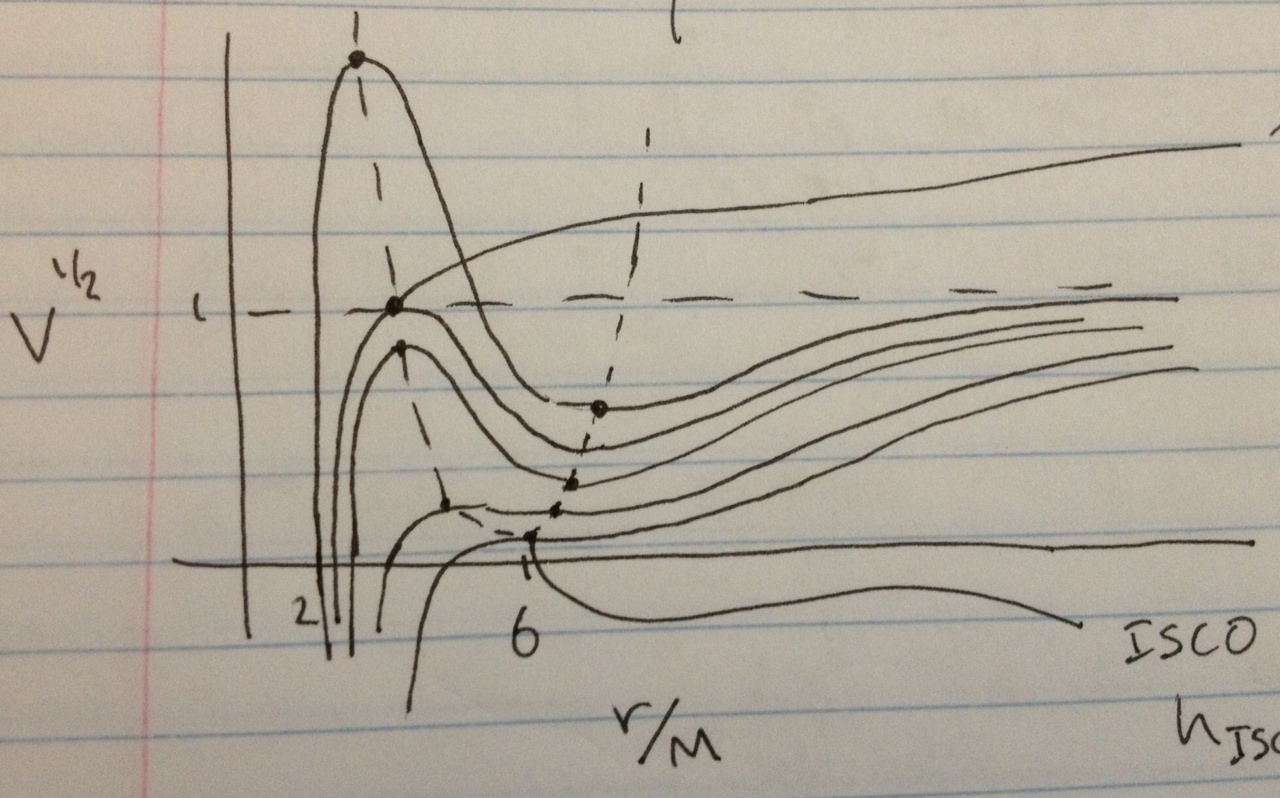
\includegraphics[width=\textwidth]{veff.jpg}
\caption{Effective potential versus radius around a Schwarzschild black hole. The innermost stable circular orbit (ISCO) is marked at $r = 6M$ \label{f:veff}}
\end{center}
\end{figure}

I have in my notes that if you have an accretion disk around your black hole, the energy you get out is the gravitational binding energy of the matter at the innermost stable circular orbit. I'm not sure why in infall from $R_{ISCO}$ doesn't count, though.


This is the potential for massive particles. For massless particles like photons, the orbits are described instead by
\begin{equation}
\biggl(\frac{dr}{d\lambda} \biggr)^2 = e^2 - \biggl( 1 - \frac{2M}{r} \biggr)  \frac{h^2}{r^2}\,\,.
\end{equation}
Here $e^2$ describes the energy and $\frac{h^2}{r^2}$ describes the momentum. Let's divide by $h^2$ to get
\begin{equation}
\frac{1}{h^2} \biggl( \frac{dr}{d\lambda} \biggr)^2 = \frac{e^2}{h^2} - \biggl( 1 - \frac{2M}{r} \biggr) \frac{1}{r^2} = \frac{1}{b^2} - \biggl( 1 - \frac{2M}{r} \biggr) \frac{1}{r^2}\,\, ,
\end{equation}
where $b$ is the impact parameter. The effect of this is that you can bend photons around black holes many times, and they can spiral around the black hole before either escaping or getting absorbed. See Figure \ref{f:veff_phot} for a plot showing the shape of the potential for photons. In this way, you can, for example, see both polar caps of a neutron star (this treatment applies outside a nonrotating NS as well), and this will affect the light curves of X-ray binaries, among other things.

\begin{figure}[!h]
\begin{center}
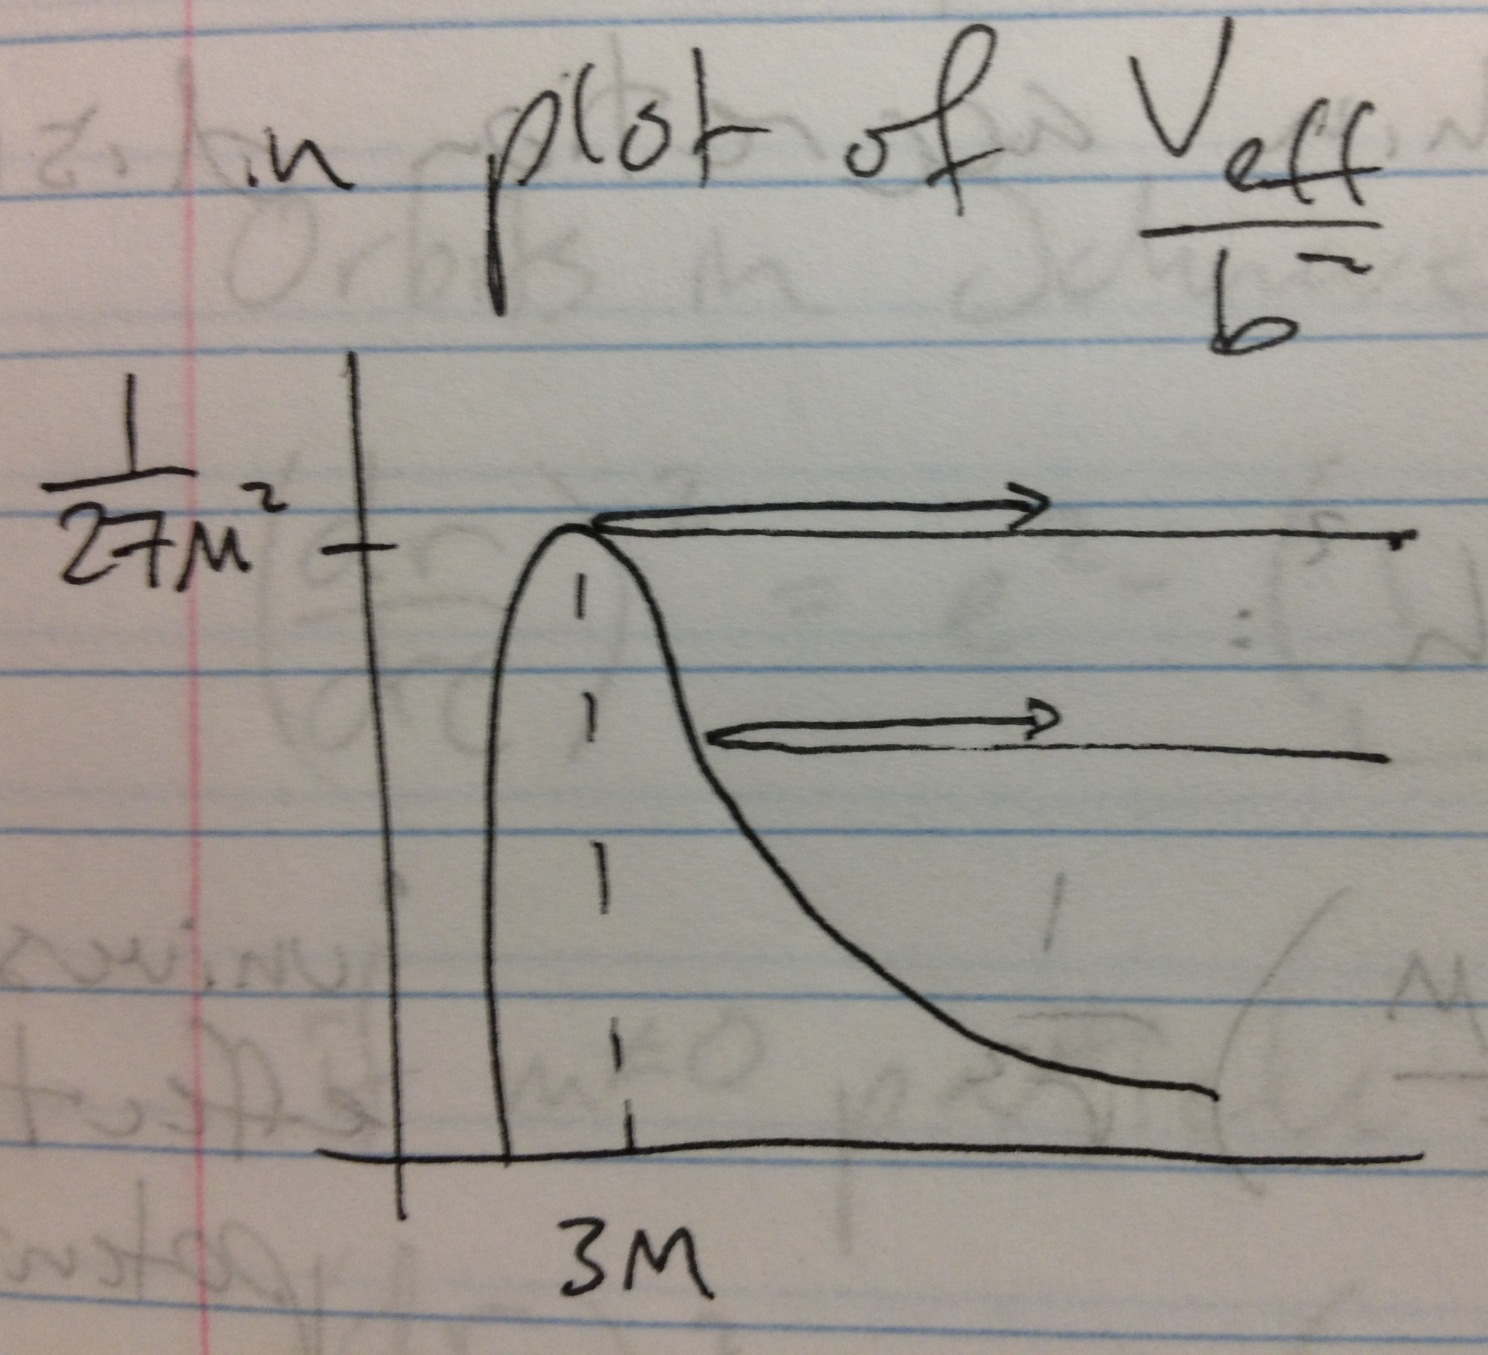
\includegraphics[width=\textwidth]{veff_phot.jpg}
\caption{Effective potential divided by squared impact parameter for a photon around a Schwarzschild black hole. The arrows show tracks of photons coming in from infinity and then escaping. The one that barely makes it to the peak will orbit the black hole many times before escaping. \label{f:veff_phot}}
\end{center}
\end{figure}

\begin{figure}[!h]
\begin{center}
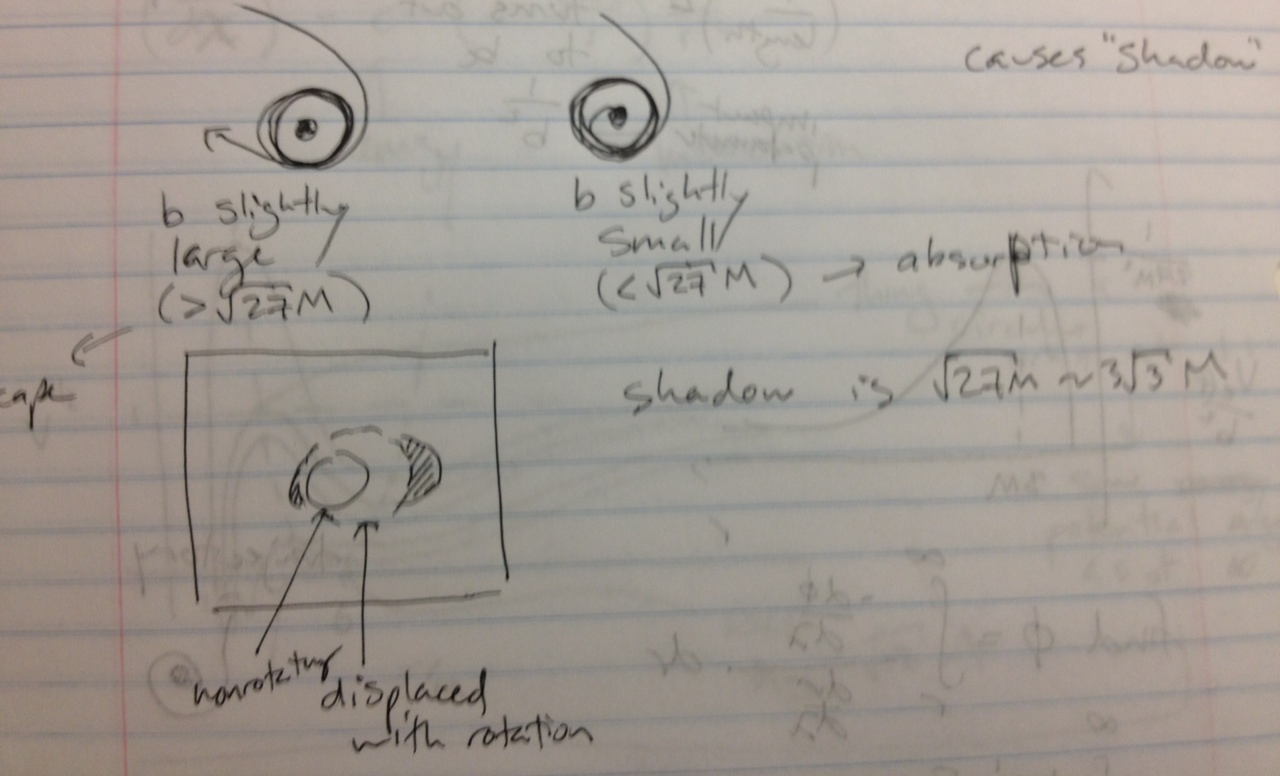
\includegraphics[width=\textwidth]{bh_shadow.jpg}
\caption{Black hole shadow. \label{f:bh_shadow}}
\end{center}
\end{figure}

Rotating Black Holes:

Hopefully we don't need to know too much about this. There's some stuff in my notes about precession as disk warping, but I'll skip it for now and maybe put it in later. The basic thing you should know is that a rotating black hole has what's called an ergosphere. The shape is basically a bulging outward from the event horizon perpendicular to the axis of rotation (so kind of like an oblate spheroid). Spacetime is dragged along with the rotation of the black hole, causing what's called ``frame dragging" (also known as the Lense-Thirring effect). This has some interesting consequences for the spins of objects in the ergosphere, and can actually spin them up or down, even though in the object's rest frame where is no torque. It is also possible to extract rotational energy from the ergosphere by dropping something into the ergosphere such that it passes through and comes back out.

The space around a rotating black hole is described by Kerr geometry. The orbit of an object described by $\Omega$ is constrained by $\Omega_{\rm min} < \Omega = \frac{d\phi}{dt} < \Omega_{\rm max}$, where
\begin{equation}
\Omega^{\rm min}_{\rm max} = \frac{ - g_{0\phi} \mp \sqrt{g_{0\phi}^2 - g_{00}g_{\phi\phi}}}{g_{\phi\phi}}
\end{equation}

\subsection{Bondi Accrection}

Bondi accrection, also called spherical accretion, assumes your central object of mass $M$ is accreting isotropically from an ambient medium at infinity with density $\rho_\infty$, temperature $T_\infty$, $v_\infty = 0$, and sound speed $c_{s\infty}^2$. We're looking for a steady state solution, so $\nabla \cdot (\rho \underline{v}) = 0$ and $\frac{1}{2} v^2 + \phi + h = {\rm constant}$, which is Bernoulli's constant. Here, $\phi = \frac{-G M}{r}$, so we're neglecting self-gravity of the accreting fluid. We also have
\begin{equation}
h = \epsilon + \frac{P}{\rho} = \frac{1}{\Gamma - 1}\frac{P}{\rho} + \frac{P}{\rho} = \frac{c_s^2}{\Gamma - 1}\,\, ,
\end{equation}
where $\Gamma = 5/3$ for monatomic gas. Let's define the Bondi radius, which separates regimes where gravity is and is not dominant:
\begin{equation}
r_B = \frac{G M}{c_{s \infty}^2} \,\,.
\end{equation}
Now let's use Bernoulli's equation to relate the quantities when the gas is at infinity to the quantities at some radius $r$:
\begin{equation}
\frac{1}{2} v_r^2 - \frac{G M}{r} + \frac{1}{\Gamma - 1} c_s^2(r) = \frac{1}{\Gamma - 1} c_{s \infty}^2
\end{equation}
since at infinity, both $v_r$ and $\phi$ go to zero. Dividing out $c_{s \infty}^2$, this equation can be rewritten as 
\begin{equation}
\frac{1}{2}\frac{v_r^2(r)}{c_s^2(r)}\frac{c_s^2(r)}{c_{s \infty}^2(r)} - \frac{r_B}{r} + \frac{1}{\Gamma - 1}\frac{c_s^2(r)}{c_{s \infty}^2(r)} = \frac{1}{\Gamma - 1}
\end{equation}
Let's define here the Mach number $\mathcal{M} = \frac{v_r^2(r)}{c_s^2(r)}$. Also write $\rho_* = \frac{\rho}{\rho_\infty}$, and this equation becomes
\begin{equation}
\frac{\Gamma - 1}{2}\mathcal{M}^2 \rho_*^{\Gamma - 1} + \rho_*^{\Gamma - 1} = 1 + \frac{\Gamma - 1}{r_*}\,\, ,
\end{equation}
where $r_* = r/r_B$. We can use the fact that $4 \pi r^2 \rho v_r = \dot{M}$ is a constant with radius to eventually solve for the Mach number as a function of radius. There are lines of solutions, which matter will follow (some are not physical), shown in Figure \ref{f:mach}. The solutions that cross the sonic point ($\mathcal{M} = 1$) represent physical accretion and wind solutions. The descending curve is for accretion, and the ascending curve is for a wind that goes supersonic.

\begin{figure}[!h]
\begin{center}
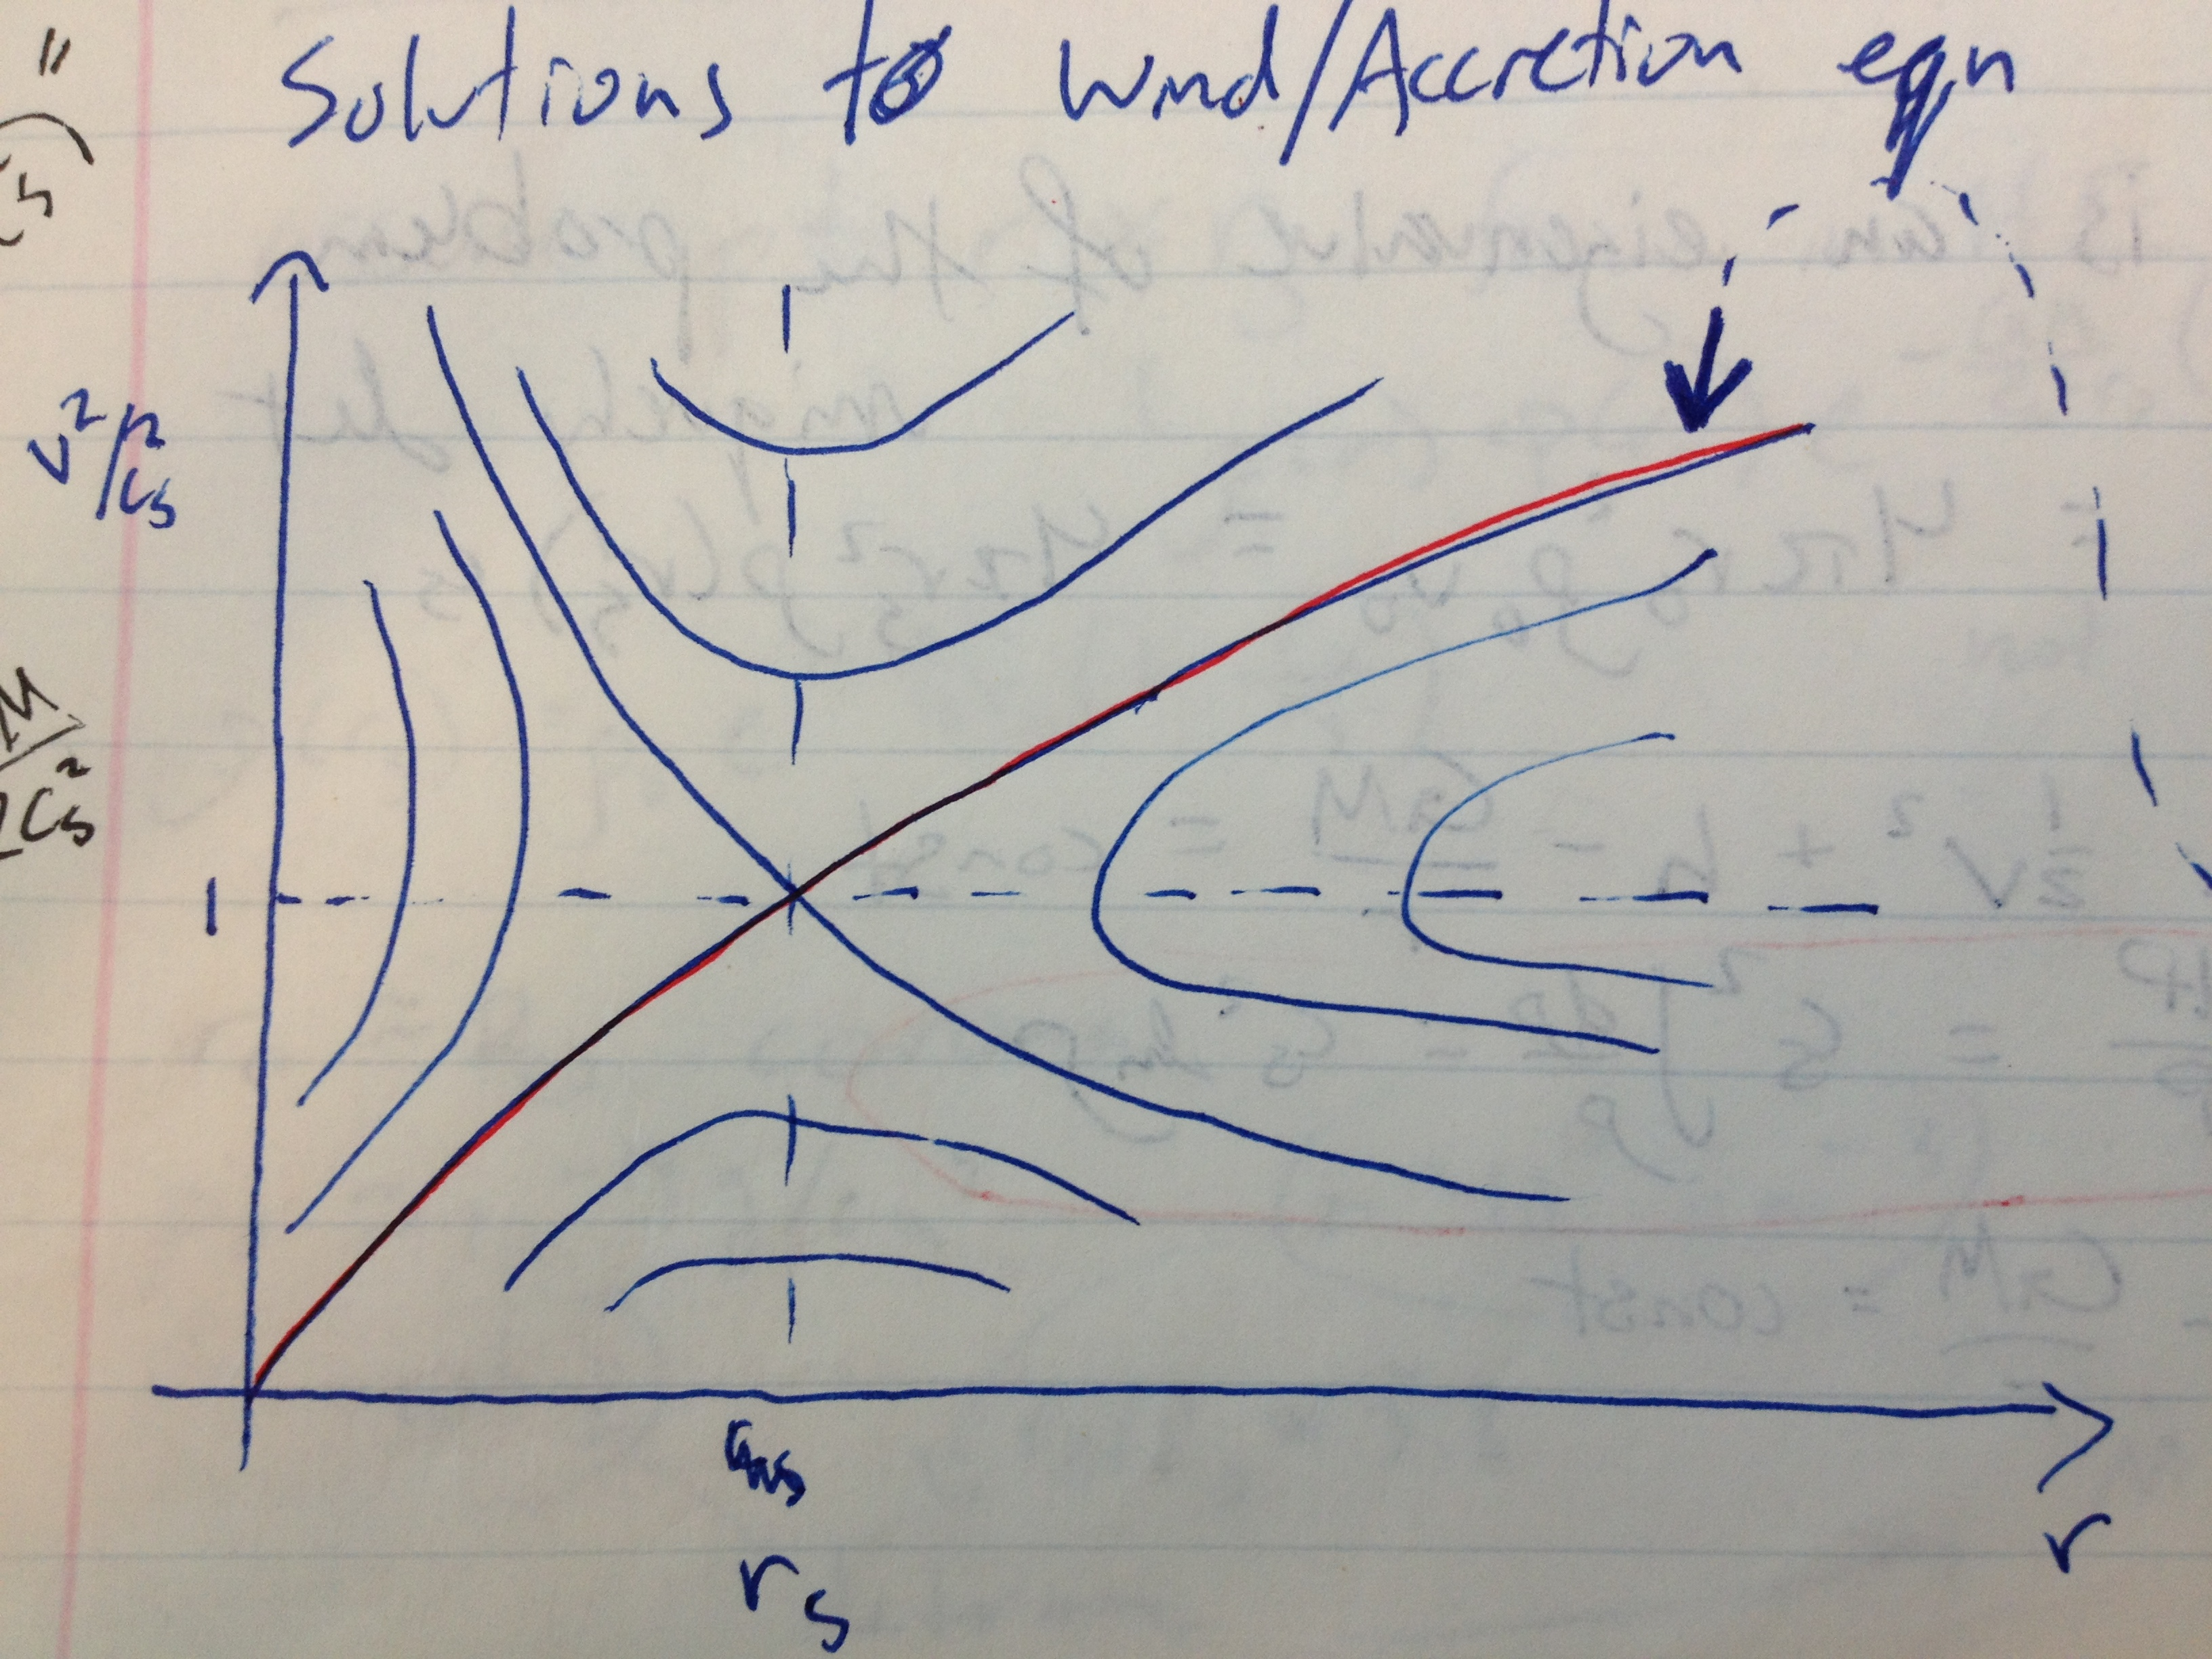
\includegraphics[width=\textwidth]{mach.jpg}
\caption{Mach number as a function of radius showing wind and accretion solutions \label{f:mach}}
\end{center}
\end{figure}

The sonic transition can be used to uniquely define $\dot{M}$:
\begin{equation}
\dot{M} = \lambda 4 \pi \biggl( \frac{G M}{c_{s \infty}^2} \biggr) ^2 \rho_\infty c_{s \infty}\,\, ,
\end{equation}
where $\lambda$ depends on $\Gamma$ and is $0.25$ for $\Gamma = 5/3$, $0.71$ for $\Gamma = 4/3$, $1.12$ for $\Gamma = 1$.

Let's also look at Bondi-Hoyle accretion, which is similar to Bondi accretion, except it's for a mass that's moving through the stuff it's accreting. This time, we can approximate:
\begin{equation}
\dot{M} = \pi \biggl(\frac{2 G M}{v_\infty ^2 + c_{s \infty}^2} \biggr)^2 \rho_* \sqrt{v_\infty ^2 + c_{s \infty}^2}\,\, .
\end{equation}
In this case, the incoming gas (from the perspective of the accreting mass) travels around the object and meets on the other side. This creates a shock in the gas, which heats and expands, and eventually this creates a bow shock around the accreting object as it moves through the fluid.

\subsection{Accretion Disks}

The idea behind accretion disks is that material falls in and maintains the angular momentum it had at large radii, so it starts to orbit the central mass. Viscosity in the disk is what causes it to heat up and radiate, which causes the material to lose energy and start falling in. Let's assume an axisymmetric situation. For Keplertian rotation, $v_\phi = \sqrt{\frac{GM}{r}}$. We can also write this as
\begin{equation}
\Omega = \Omega_K = \sqrt{\frac{GM}{r^3}}\,\,.
\end{equation}

The disk is characterized by its surface density $\Sigma$, which is the mass density $\rho$ integrated vertically. Assuming symmetry in the $\phi$ direction, an annulus defined as the disk material between $r$ and $r+dr$ has a mass $2 \pi r dr \Sigma$ and angular momentum $2 \pi r dr \Sigma r^2 \Omega$. 

Because the velocity decreases with radius, we can imagine a thin ring of the disk with an adjacent interior ring moving more slowly and an adjacent outer ring moving more quickly. Imagine elements in these three rings for temporary `bonds' with each other, so the inner ring gets pulled back and bit and the outer ring gets pushed forward a bit due to the interaction between the rings (which is due to viscosity). Actually, the lowest energy state that the disk is trying to get to is one in which a small part of the mass goes out to infinity and carries all the angular momentum with it, while the rest of the accretion disk falls into the accretor. We can approximate the viscosity as
\begin{equation}
\nu \sim \lambda v_{th}\,\, ,
\end{equation}
where $\lambda$ is the distance between our two layers and $v_{th}$ is the speed of whatever is mediating the interaction. For molecular transport, $\lambda$ is the mean free path and $v_{th}$ I have already denoted as the thermal speed of the particles. The torque of the inner layer on the outer layer is
\begin{equation}
T(r) = 2 \pi r \nu \Sigma r^2 \Omega^\prime
\end{equation}
where $ \Omega^\prime = \frac{\partial \Omega}{\partial r}$. The viscous torques cause a dissipation at a rate $T \Omega^\prime dr$ for a ring with width $dr$. The rate per area of the ring is $D(r)$, and it can be found by dividing this area by $2 \times 2\pi r dr$, where the extra factor of $2$ comes from the ring having two sides, top and bottom. Then
\begin{equation}
D(r) = \frac{T \Omega^\prime}{4 \pi r}  = \frac{1}{2} \nu \Sigma (r \Omega^\prime)^2
\end{equation}
Let's assume the orbital frequency is Keplerian, so $\Omega^\prime = \sqrt{GM/R^3}$. Then
\begin{equation}
D(r) \ frac{9}{8} \nu \Sigma \frac{GM}{r^3}\,\,.
\end{equation}

Now let's look at the case of the steady thin disk. In this case, $\dot{M} = 2 \pi r \Sigma (-v_r)$ is constant. Using the momentum equation gives
\begin{equation}
r \Sigma v_r r^2 \Omega = \frac{T}{2 \pi} + {\rm constant}\,\,.
\end{equation}
Plugging in for $T$ gives
\begin{equation}
-\nu \Sigma \Omega^\prime = -v_r\Sigma \Omega + {\rm constant}\,\,.
\end{equation}
We need to find the constant by considering the disk down at the surface of the star or compact object $R_*$. The central object should be rotating at less than breakup speed, so $\Omega_* < \Omega_K$. Therefore the disk is Keplerian in the outer layers, but as we go inward in radius, it must eventually decrease to the rotation speed of the star.

One good thing to know about an accretion disk is its thickness. The scale height $H$ provides a measure of the thickness when compared with the radius $R$. It's possible to approximate the scale height by using hydrostatic equilibrium in the $z$ direction:
\begin{equation}
\frac{dP}{dz} = -g_z \rho = -\frac{GM}{r^2} \frac{z}{r}\,\,.
\end{equation}
We can hand-wave this by setting $dz = z = H$ and $r = R$ and using ideal gas for $P$:
\begin{equation}
H \sim \biggl( \frac{k_{\rm B} T R^3}{GM m_p}\biggr)^{1/2}\,\,.
\end{equation}
Typical temperatures are around $10^4~{\rm K}$.

Now let's define the surface mass density $\Sigma(r) = \int^\infty_{-\infty} \rho dz$. We can get the average velocity $\langle v_r \rangle$ by integrating $v_r$ over $z$ and $\phi$ in a mass-weighted way. Then we can get the accretion rate,
\begin{equation}
\dot{M} = 2 \pi r \Sigma \langle v_r \rangle\,\, ,
\end{equation}
which is constant with $r$.

For an accretion disk, the mass conservation equation turns out to be
\begin{equation}
r \frac{\partial \Sigma}{\partial t} + \frac{\partial}{\partial r} (r \Sigma v_r) = 0\,\,,
\end{equation}
and conservation of momentum is
\begin{equation}
f \frac{\partial}{\partial t} (\Sigma r^2 \Omega)
\end{equation}

\subsection{High-Energy Binaries}

\subsection{GRBs}

\subsection{AGN}

\subsection{Cosmic Rays}

\section{Instrumentation}
\subsection{Questions}
\begin{enumerate}
\item \textbf{Describe quantitatively the point spread function of a diffraction-limited optical
      telescope. Explain how diffraction spikes arise, and what determines their positions
      and intensities. Under what circumstances will the PSF be broadened by atmospheric
      turbulence?}
\item \textbf{Derive an expression for the point source sensitivity of a radio interferometer as
      a function of the frequency, bandwidth, system temperature, diameter of each dish,
      number of dishes, etc.}

      \newthought{Let's begin by} deriving the point source sensitivity of a single dish
      radio telescope.  To do so, we need a little bit of background on what a radio telescope
      is.  There are two broad classes of single-dish radio telescopes: those with coherent
      detectors and those with incoherent detectors.  Coherent detectors measure the amplitude
      and phase of the incoming electric field, while incoherent detectors discard the phase
      information.  In this way, incoherent detectors are essentially very sensitive thermometers.
      We will focus this discussion on coherent detectors (because the phase information is needed
      for interferometry).

      A radio telescope can be broken down into a number of parts.  We will consider these
      parts in the order that they translate the sky brightness into a brightness temperature.
      \begin{itemize}
      \item The antenna and feed

            First, there must be a component that is sensitive to a time varying electric
            field.  The feed converts the time varying electric field into a time varying voltage.
            This can be a massive dish with a feed at its focus, or merely a
            simple piece of wire acting as a dipole antenna.  Obviously the large dish will
            be very sensitive in the forward direction, while the simple dipole antenna will
            be sensitive to almost the entire sky, but not particularly sensitive in any one
            direction.  The pattern of sensitivity for an antenna is called its ``gain pattern''.
            The higher the gain in a given direction, the more sensitive the antenna is to signals
            from that direction.  This gain pattern is typically encoded in the ``effective
            collecting area'' of the antenna.

            It can be shown that for any antenna the angle-averaged effective collecting area
            is given by
            \begin{dmath}\label{eq:Ae}
                \langle A_e\rangle = \frac{\lambda^2}{4\pi}
            \end{dmath},
            where $\lambda$ is roughly the central wavelength of the bandpass.  We can get
            an intuitive understanding for why this equation must be true by comparing the
            100 m Green Bank telescope with a simple LWA dipole.  The Green Bank telescope
            has a $\pi(50~{\rm m})^2 \approx 8000~{\rm m}^2$ collecting area in its forward
            direction, and a low (but nonzero) sensitivity in the off-axis directions coming
            in through the telescope's sidelobes.  Averaging over all angles reproduces
            Equation~\ref{eq:Ae}.  On the other hand, the LWA dipoles are roughly evenly
            sensitive to the whole sky.  Therefore, at $\lambda=10~{\rm m}$ each dipole has
            an effective collecting area of $\approx 8~{\rm m}^2$ towards all parts of the sky.

            Finally, it should be noted that an antenna can only be sensitive to one polarization
            of light.  Therefore, in order to measure the total power from a source one must
            build two feeds so that one is sensitive to each polarization.

      \item The receiver

            The receiver is a general term for the electronics that process the signal coming
            from the feed.  For a radiometer\sidenote{
                A radiometer simply measures the total power in the voltage fluctuations coming
                from the feed.
            }, the receiver will consist of (in its simplest design):
            a gain stage to amplify the signal,
            a bandpass filter to restrict the signal to a known frequency range,
            a square law detector that produces a voltage output proportional to the total
            power\sidenote{
                $V_{\rm out} \propto V_{\rm in}^2$
            }, and an integrator that accumulates the voltage samples over a given time.

            Additionally, most radiometers include electronics to stabilize the gain of the
            amplifiers, analog to digital converters that sample and digitize the signal\sidenote{
                Digital signals are less likely to deteriorate as they pass through lossy cable.
                However the digitization process itself is lossy and can restrict the dynamic
                range of the telescope if not enough bits are used to represent the signal.
                The rate at which an ADC must sample is determined by the Nyquist frequency.
            }, and a mixer that converts high frequency signals into low frequency signals
            that are easier to process electronically.
      \end{itemize}

      Now let's assume we have an antenna with a bandwidth $B$ (set by the bandpass filter),
      integration time $\tau$.  After the integrator we have an estimate for the system
      temperature $T_{\rm sys} = P_\nu/k$, where $P_\nu$ is the power per unit frequency in the
      antenna and $k$ is the Boltzmann constant.  With an ADC sampling at the Nyquist frequency,
      the integrator uses $2B\tau$ independent samples of the power to estimate $T_{\rm sys}$.
      Therefore, the uncertainty on the measurement of $T_{\rm sys}$ is
      \begin{dmath*}
        \sigma_T = \frac{\sigma_{T,0}}{\sqrt{2B\tau}}
      \end{dmath*},
      where $\sigma_{T,0}$ is the uncertainty on a single sample of $T_{\rm sys}$.  To derive
      $\sigma_{T,0}$ we use the fact that $T_{\rm sys} \propto \langle V^2\rangle$ where $V$
      is the voltage before the square-law detector.  Setting the constant of proportionality
      to unity we have
      \begin{dmath*}
        \sigma_{T,0}^2 = \langle V^4\rangle - \langle V^2\rangle^2
                       = \frac{1}{\sqrt{2\pi T_{\rm sys}}}\int_{-\infty}^{+\infty} V^4e^{-V^2/2T_{\rm sys}}\,\d V
                       - \left(\frac{1}{\sqrt{2\pi T_{\rm sys}}}\int_{-\infty}^{+\infty} V^2e^{-V^2/2T_{\rm sys}}\,\d V\right)^2
                       = 3T_{\rm sys}^2 - T_{\rm sys} \nolinebreak = 2T_{\rm sys}
      \end{dmath*}.
      Therefore we have derived the radiometer equation, which describes the temperature
      sensitivity of a single dish radio telescope:
      \begin{dmath}\boxed{
        \sigma_T = \frac{T_{\rm sys}}{\sqrt{B\tau}}
      }\end{dmath}

\item \textbf{Describe some of the common technologies for detecting gamma rays, the approximate
      energy range over which they are applicable, and some of their main advantages
      and disadvantages.}
\end{enumerate}


\end{document}

